\documentclass[oneside, 12pt]{book}

% ------------------------------------------------------------------------------
% Setup for table of contents
\setcounter{tocdepth}{3} 	% TOC should label down to subsubsections
\setcounter{secnumdepth}{2}	% TOC should not number further than a subsection number
% ------------------------------------------------------------------------------


% ------------------------------------------------------------------------------
% General Setup
\usepackage[english]{babel}
\usepackage{amsfonts, amsmath, amsthm, amssymb}		% Formatting symbols, theorems, lemmas, definitions, and examples

\usepackage{float}							% For making sure tables and figures stay in place
\usepackage{fullpage}						% Create ~1" margins
\usepackage{changepage}						% For setting up indents after examples
\usepackage[bottom,flushmargin]{footmisc}	% Put footnotes at bottom of page; don't intent footnotes
\usepackage[titletoc]{appendix}

\setcounter{chapter}{-1}				% Start with chapter 0

\usepackage{enumitem}					% For custom labels on enumerations
\usepackage{hyperref}					% For inserting links
\usepackage{graphicx} 					% For inserting images

% Tikz stuff
\usepackage{tikz}
\usetikzlibrary{patterns}
\usetikzlibrary{calc,patterns,decorations.pathmorphing,decorations.markings}
% ------------------------------------------------------------------------------

% ------------------------------------------------------------------------------
% Theorems, corollaries, definitions, lemmas, and examples should not be numbered
\newtheorem*{theorem}{Theorem}
\newtheorem*{corollary}{Corollary}
\newtheorem*{definition}{Definition}
\newtheorem*{lemma}{Lemma}
% ------------------------------------------------------------------------------

% ------------------------------------------------------------------------------
% Examples are not numbered. However, the answers that follow examples are indented and have an extra line break.
\newtheorem*{example}{Example}
\newenvironment{answer}{\begin{adjustwidth}{15pt}{}}{\end{adjustwidth}}
% ------------------------------------------------------------------------------

% ------------------------------------------------------------------------------
% Don't indent paragraphs by default
\setlength{\parindent}{0pt}
% ------------------------------------------------------------------------------

% ------------------------------------------------------------------------------
% Shortcuts
\newcommand{\dd}[2]{\frac{\mathrm{d} #1}{\mathrm{d} #2}}							% d[] / d[]
\renewcommand{\d}[1]{\mathrm{d} #1}
\renewcommand{\qedsymbol}{$\blacksquare$}
\newcommand{\abs}[1]{\big\lvert #1 \big\rvert}												% absolute value

\DeclareMathOperator{\arcsec}{arcsec}												% arc-secant
\DeclareMathOperator{\arccot}{arccot}												% arc-cotangent
\DeclareMathOperator{\arccsc}{arccsc}												% arc-cosecant

\newcommand{\R}{\mathbb{R}}															% Real numbers
% ------------------------------------------------------------------------------

\begin{document}
	% Title page setup
	\title{Single Variable Calculus: A Summary}
	\author{William Boyles}
	\date{}
	
	\frontmatter
		\maketitle
		\tableofcontents
		
	\mainmatter
		\chapter{Background \& Review}
Everything mentioned in this chapter should already be familiar to you from other math classes.
These topics span two major areas: algebra/pre-calculus and limits.
Ideas from these topics will often be used implicitly or without a passing reference. \\

If you are unfamiliar with anything mentioned, you can use many of the great online resources like Khan Academy to familiarize yourself before moving forward.

\section{Algebra and Pre-Calculus}
\noindent

\subsection{Sets}
\begin{definition}
	A set $A$ is a collection of distinct elements. Those elements can be anything, like numbers, functions, and even other sets.
\end{definition}
We can define a set by giving its elements, like $A = \{-2, 5, 3\}$ or by describing its properties, like $A = \{x \mid x > 0\}$ where the vertical bar means "such that".
If an object $x$ is a member of the set $A$, we write $x\in A$.\bigskip


\noindent
A set $A$ is called a subset of a set $B$ if every element of $A$ is also an element of $B$. 
We can write this as $A \subseteq B$. 
For example, $\{7, 10, 16\} \subseteq \{5, 6, 7, 9, 10, 11, 16\}$. 
Note that this relation can be strict if there exists at least one element in $B$ that is not also an element of $A$. 
Some common sets and their informal definitions are given below:

\begin{table}[H]
	\centering
	\begin{tabular}{c|c|c}
		Set Name & Symbol & Informal Definition                                                                                                                         \\ \hline
		Natural numbers & $\mathbb{N}$ & $\{1, 2, 3, \dots\}$           						                                                                        \\
		Integers & $\mathbb{Z}$ & $\{\dots, -3, -2, -1, 0, 1, 2, 3, \dots\}$                                                                                            \\
		Rational numbers & $\mathbb{Q}$ & $\{\frac{m}{n} \mid m,n \in\mathbb{Z}$ and $n \neq 0\}$                                                                       \\
		Real numbers & $\mathbb{R}$ & Any number on the number line\footnote{Sadly, there is no way to give a stronger formal definition without higher mathematics.}   \\
	\end{tabular}
\end{table}

This means that $\mathbb{N} \subset \mathbb{Z} \subset \mathbb{Q} \subset \mathbb{R}$.\bigskip


\noindent
There are several common operations that can be performed on sets.
The union $A \cup B$ of two sets $A$ and $B$ is the set of all elements that are elements of $A$ or of $B$. 
Similarly, the intersection $A \cap B$ of two sets $A$ and $B$ is the set of all elements that are also elements of both $A$ and $B$.
\begin{example}
	If $A = \{\sqrt{2}, 2, 5, 8\}$ and $B = \{-9, 8, 2.3\}$, what are $A \cup B$ and $A \cap B$?		
\end{example}
To find the union, we combine the sets, making sure to include any repeated element only once:
\begin{equation*}
	A \cup B = \{-9, \sqrt{2}, 2, 2.3, 5, 8\}.
\end{equation*}
Then, since the only element both sets share is 8, we also have
\begin{equation*}
	A \cap B = \{8\}.
\end{equation*}

\subsection{Intervals}
\begin{definition}
	We call a subset $I$ of $\mathbb{R}$ an interval if, for any $a, b \in I$ and $x \in \mathbb{R}$ such that $a \leq x \leq b$, then $x \in I$. 
\end{definition}
We can write an interval more simply using the notation $[a, b]$, which is equivalent to $\{x \in \mathbb{R} \mid a \leq x \leq b\}$. 
This is called a closed interval, and to make the inequalities strict, we can also define an open interval by using parantheses instead of square brackets.\bigskip

In addition, we can mix the two to create half-open intervals, where one inequality is strict and the other isn't. 
For instance, $(2, 5]$ refers to the set $\{x \in \mathbb{R} \mid x < 2 \leq 5\}$
Finally, if the interval is unbounded in either direction, we use the notations $-\infty$ and $\infty$ to indicate that there is no minimum or maximum, respectively.

\begin{example}
	Is $8 \in (-\infty, 4) \cup [8, 100)$?
\end{example}
\begin{answer}
	Since $8 \leq 8 < 100$ is a true statement, $8 \in [8, 100)$. 
	Since we are taking the union with another set, all of the members of the right interval will also be members of the union of intervals. 
	Therefore, the statement is true.
\end{answer}                       % Sets
\subsection{Functions}
\begin{definition}
    A function $f$ is a rule between a pair of sets, denoted $f: D \to C$, that assigns values from the first set, the domain $D$, to the second set, the codomain $C$.
\end{definition}

We call the subset of the codomain $C$ that constitutes all values $f$ can actually attain the range $R \subseteq C$. 
Note that when we draw a graph of a function, all we are doing is drawing all ordered pairs $\{(x, f(x)) \mid x \in D\}$.

\begin{example}
    Find the domain of the following function:
    \begin{equation*}
        f(x) = \frac{1}{(1 - x)\sqrt{5 - x^2}}
    \end{equation*}
\end{example}

\begin{answer}
    We know that $\frac{n}{0}$ is undefined for all $n \in \mathbb{R}$ and $\sqrt{x}$ is only defined for $x \geq 0$. 
    The first condition applies to the first term in the denominator and both conditions apply to the second, giving us
    \begin{equation*}
        (1 - x) \neq 0 \text{ and } 5 - x^2 > 0
    \end{equation*}
    The first condition implies $x \neq 1$ while the second implies $|x| < \sqrt{5}$.
    Putting these together, we find that the domain is
    \begin{equation*}
        \{x \mid x \neq 1, |x| < \sqrt{5}\} \text{ or } (-\sqrt{5}, 1) \cup (1, \sqrt{5})
    \end{equation*}
\end{answer}

We can also compose two functions, such that the ouput of one function is the input of another: 
\begin{equation*}
    (f \circ g)(x) = f(g(x)).
\end{equation*}

\begin{definition}
    A function $g$ is called an inverse function of $f$ if $f(g(x)) = x$ for all x in the domain of g and $g(f(x))$ for all x in the domain of f. 
    We write this as $g = f^{-1}$.
\end{definition}

One common algorithm for finding an inverse function is to set $y = f(x)$, substitute all $x$'s for $y$'s, and then solve for y.
\begin{example}
    Find the inverse function of 
    \begin{equation*}
        f(x) = \frac{5x + 2}{4x - 3}.
    \end{equation*}
\end{example}
\begin{answer}
    We first make the substitutions to set up the algorithm:
    \begin{equation*}
        y = \frac{5x + 2}{4x - 3} \text{ followed by }
        x = \frac{5y + 2}{4y - 3}
    \end{equation*}
    After multiplying both sides by the denominator and simplifying, we have
    \begin{equation*}
        \implies 4xy - 3x = -5y - 2 \\
        \implies y = f^{-1}(x) = \frac{3x - 2}{4x + 5}.
    \end{equation*}
\end{answer}

We say that a function $f$ is even if it satisfies $f(-x) = f(x)$ for all $x \in D$.
Likewise, we say that a function $f$ is odd if it satisfies $f(-x) = -f(x)$ for all $x \in D$. 
Geometrically, we can see that the graph of an even function is symmetric with respect to the $y$-axis, while the graph of an odd function is symmetric with respect to the origin. 

\begin{example}
    Is $f(x) = 2x - x^2$ even, odd, or neither?
\end{example}
\begin{answer}
    \begin{equation*}
        f(-x) = 2(-x) - (-x)^2 = -2x - x^2
    \end{equation*}
    Since $f(-x) \neq f(x)$ and $f(-x) \neq -f(x)$, the function is neither even nor odd.
\end{answer}                   % Functions
\subsection{Complex Numbers}
\begin{definition}
	$i$ is called the imaginary unit. It's defined by $i^2 = -1$.
\end{definition}


\noindent
Complex numbers ($\mathbb{C}$) have the form $z = \alpha + \beta i$, where $\alpha$ and $\beta$ are real numbers. The $\alpha$ part of $z$ is called the real part, so $\Re(z) = \alpha$. The $\beta$ part of $z$ is called the imaginary part, so $\Im(z) = \beta i$.\\

\noindent
Often, complex numbers are visualized as points or vectors in a 2D plane, called the complex plane, where $\alpha$ is the x-component, and $\beta$ is the y-component. Thinking of complex numbers like points helps us define the magnitude of complex numbers and compare them. Since a point $(x,y)$ has a distance $\sqrt{x^2+y^2}$ from the origin, we can say the magnitude of $z$, $\lvert z \rvert$ is $\sqrt{\alpha^2 + \beta^2}$. Thinking of complex numbers like vectors helps us understand adding two complex numbers, since you just add the components like vectors.\\

\noindent
A common operation on complex numbers is the complex conjugate. The complex conjugate of $z = \alpha + \beta i$ is $\overline{z} = \alpha - \beta i$. $z$ and $\overline{z}$ are called a conjugate pair.\\

\noindent
Conjugate pairs have the following properties.
Let $z, w \in \mathbb{C}$.
\begin{align*}
	\overline{z \pm w} &= \overline{z} \pm \overline{w} \\
	\overline{zw} &= \overline{z}\overline{w} \\
	\overline{z} &= z \Leftrightarrow z \in \mathbb{R} \\
	z\overline{z} &= \lvert z \rvert^2 = \lvert \overline{z} \rvert^2 \\
	\overline{\overline{z}} &= z \\
	\overline{z}^n &= \overline{z^n} \\
	z^{-1} &= \frac{\overline{z}}{\lvert z \rvert^2} 
\end{align*}
 			% Complex Numbers
\subsection{Factoring Polynomials}
\noindent
We want to break up a polynomial like $f(x) = a_0 + a_1x^1 + \ldots a_nx^n$ into linear factors so that $f(x) = c(x-b_1)\cdot \ldots \cdot(x - b_n)$. This form makes it simple to see that the roots of $f$, solutions to $f(x) = 0$, are $x = b_1 \ldots b_n$.\\

\noindent
For quadratics, $f(x) = ax^2 + bx + c$, there exists a simple formula that will give us both roots, the quadratic formula
\begin{equation*}
	x = \frac{-b \pm \sqrt{b^2-4ac}}{2a}.
\end{equation*}

\noindent
We can see that when $b^2 - 4ac < 0$, like for $f(x) = x^2 + 5x + 10$, we will get complex roots $\alpha \pm \beta i$. For any polynomial, these roots come in pairs, so if $\alpha + \beta i$ is a root, then so is $\alpha - \beta i$. This means that every conjugate pair $\alpha \pm \beta i$ has a quadratic equation with those roots. Sometimes we will not factor quadratics with complex roots into linear terms.\\

\noindent
Although there do exist explicit formulas for finding roots for cubic (degree 3) and quartic (degree 4) equations, they are too long and not useful enough to memorize. When working by hand, we instead use other tricks to find roots.\\

\noindent
There are a few useful tricks that can help. If the polynomial doesn't have a constant term, then 0 is a root. If all the coefficients sum to 0, then 1 is a root. For certain polynomials with an even number of terms, like all cubics of the form $ax^3 + bx^2 + cax + cb$ we can factor out a term from the first two and last two terms to get $x^2(ax+b)+c(ax+b) = (ax+b)(x^2+c)$. For other polynomials, we might just try guessing and checking values. However, we need a more efficient way that works in general.\\

\noindent
Since we are looking to find linear factors $f(x) = (x-b_1)\cdot \ldots \cdot(x-b_n)$, we can see that the constant term in the polynomial is the product of the roots $b_1 \ldots b_n$. In fact, since the coefficients of polynomials are completely determined by the roots and the leading coefficient, all the coefficients are sums and products of roots. You might remember when factoring quadratics that the coefficient of $x$ term is the sum of the two roots. These rules are called Vieta's formulas.\\

\noindent
So, if we have the constant term, we can check all of its integer factors to see if any are roots. For each root, we can divide, using a technique like synthetic division, to continue finding the rest of the roots. This method is especially useful on tests because the roots tend to be integers.

\input{../common/algebraPreCalc/factoringPolynomials_example.tex} 		% Factoring Polynomials
\subsection{Trig Functions \& The Unit Circle}
\noindent
Imagine aa circle of radius 1 centered at the origin that we'll call the unit circle. The x and y coordinates of a point on the unit circle are completely determined by the angle $\theta$ in radians between the $x$-axis and a line from the origin to the point.\\

\noindent
The function $\cos{\theta}$ tells us x-coordinate of the point, while $\sin{\theta}$ tells us the y-coordinate of the point. The function $\tan{\theta} = \frac{\sin{\theta}}{\cos{\theta}}$ tells us the slope of the line from the origin to the point. Most of the trig functions have geometric interpretations as shown below. The most used ones are $\sin$, $\cos$, $\tan=\frac{\sin}{\cos}$, $\cot = \frac{\cos}{\sin}$, $\csc=\frac{1}{\sin}$, and $\sec=\frac{1}{\cos}$.

\begin{figure}[H]
	\label{unitCircle}
	\centering
	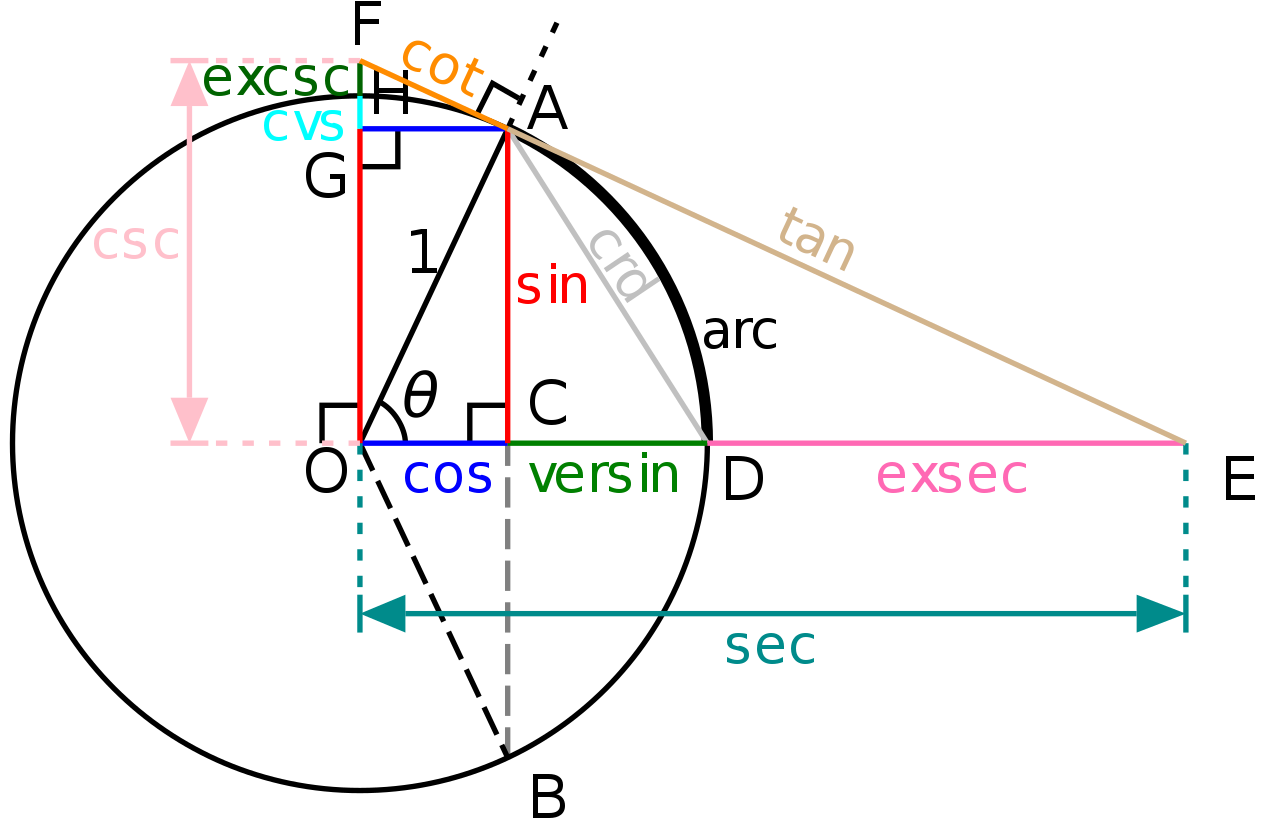
\includegraphics[width = 0.75\textwidth]{../common/algebraPreCalc/unitCircle2.png}
	\caption{\hyperref{https://en.wikipedia.org/wiki/Unit_circle}{}{}{Wikipedia - Unit circle}}
\end{figure}

\noindent
We can also think about the inverses of these trig functions. These are either notated with a -1 exponent on the function, or the prefix arc in front of the function name. Many of these functions are only defined on a part of the domain $\left[0, 2\pi\right]$. Below is a table of the inverse trig functions and their domains.

\begin{table}[H]
	\centering
	\begin{tabular}{l|l}
		Function  & Domain                                                 \\ \hline
		$\arcsin$ & $\left[-1, 1\right]$           						   \\
		$\arccos$ & $\left[-1, 1\right]$                                   \\
		$\arctan$ & $\left(-\infty, \infty\right)$                         \\
		$\arccot$ & $\left(-\infty, \infty\right)$                         \\
		$\arccsc$ & $\left(-\infty, -1\right] \cup \left[1, \infty\right)$ \\
		$\arcsec$ & $\left(-\infty, -1\right] \cup \left[1, \infty\right)$
	\end{tabular}
\end{table}
 	% Trig Functions / Unit Circle
\subsection{Trig Identities}
\noindent
As we could see in Figure \ref{unitCircle}, $\sin$ and $\cos$ form a right triangle with hypotenuse 1. So, using the Pythagorean Theorem,
\begin{equation*}
	\sin^2{\theta} + \cos^2{\theta} = 1.
\end{equation*}
By dividing by $\sin^2$ or $\cos^2$, we can also get
\begin{equation*}
	1 + \cot^2{\theta} = \csc^2{\theta} \text{ and } \tan^2{\theta} + 1 = \sec^2{\theta}.
\end{equation*}
Together, these 3 identities are called the Pythagorean Identities.\\

\noindent
We can also relate functions and co-functions.
\begin{equation*}
	\text{xxx}(\theta) = \text{coxxx}\left(\frac{\pi}{2} - \theta\right).
\end{equation*}

\noindent
Some of the most useful and used identities are the sum and difference.
\begin{align*}
	\sin{\left(\alpha \pm \beta\right)} &= \sin{\alpha}\cos{\beta} \pm \cos{\alpha}\sin{\beta} \\
	\cos{\left(\alpha \pm \beta\right)} &= \cos{\alpha}\cos{\beta} \mp \sin{\alpha}\sin{\beta} \\
	\tan{\left(\alpha \pm \beta\right)} &= \frac{\tan{\alpha} \pm \tan{\beta}}{1 \mp \tan{\alpha}\tan{\beta}} \\
	\sin{\alpha} \pm \sin{\beta} &= 2\sin{\left(\frac{\alpha \pm \beta}{2}\right)}\cos{\left(\frac{\alpha \mp \beta}{2}\right)} \\
	\cos{\alpha} + \cos{\beta} &= 2\cos{\left(\frac{\alpha + \beta}{2}\right)}\cos{\left(\frac{\alpha - \beta}{2}\right)} \\
	\cos{\alpha} - \cos{\beta} &= -2\sin{\left(\frac{\alpha + \beta}{2}\right)}\sin{\left(\frac{\alpha - \beta}{2}\right)} \\
\end{align*} 			    % Trig Identites
\subsection{Exponentials \& Logarithms}
\begin{definition}
	e is the base of the natural logarithm. It's defined by the limit
	\begin{equation*}
		e = \lim\limits_{n\rightarrow\infty}{\left(1+\frac{1}{n}\right)^n}.
	\end{equation*}
\end{definition}
\noindent
$\exp{x} = e^x$ and $\ln{x}$ are inverse functions of each other such that
\begin{equation*}
	e^{\ln{x}} = x \text{ and } \ln{e^x} = x.
\end{equation*}

\noindent
Just like other exponentials, the normal rules for adding, subtracting, and multiplying exponents apply:
\begin{equation*}
	e^xe^y = e^{x+y} \text{, } \frac{e^x}{e^y}=e^{x-y} \text{, and } \left(e^x\right)^k=e^{xk}.
\end{equation*}

\noindent
Similar rules apply for logarithms:
\begin{equation*}
	\ln{x}+\ln{y} = \ln{xy} \text{, } \ln{x}-\ln{y} = \ln{\left(\frac{x}{y}\right)} \text{, and } \ln{\left(a^b\right)} = b\ln{a}.
\end{equation*}

\noindent
We can also write a logarithm of any base using natural logarithms:
\begin{equation*}
	\log_{b}{a} = \frac{\ln{a}}{\ln{b}}.
\end{equation*}

\noindent
$e$ is also unique in that it is the only real number $a$ satisfying the equation
\begin{equation*}
	\frac{\mathrm{d}}{\mathrm{d}x}a^x = a^x,
\end{equation*}
meaning $e^x$ is its own derivative. 		% Exponential and logarithms
\subsection{Partial Fractions}
\noindent
If we have a function of two polynomials $f(x) = \frac{P(x)}{Q(x)}$, it's often easier to break this quotient into a sum of parts where the denominator is a linear or quadratic factor and the numerator is always a smaller degree than the denominator.

\begin{example}
	\begin{equation*}
		\frac{2x-1}{x^3-6x^2+11x-6} = \frac{1/2}{x-1}+\frac{-3}{x-2}+\frac{5/2}{x-3}.
	\end{equation*}
\end{example}

\noindent
One natural way to find these small denominators comes from the linear factors of the denominator where we keep quadratics with complex roots.
This way, when making a common denominator, we get back the original big denominator.
However, there are a few special cases we have to take care of.

\input{../common/algebraPreCalc/linearFactors.tex}
\input{../common/algebraPreCalc/repeatedLinearFactors.tex}
\input{../common/algebraPreCalc/quadraticFactors.tex}
\input{../common/algebraPreCalc/repeatedQuadraticFactors.tex}
\input{../common/algebraPreCalc/improperFractions.tex}
 			% Partial Fractions % Algebra and Pre-Calc
		\chapter{Limits \& Continuity}

Limits are a way of describing what happens to a function $f(x)$ as $x$ gets arbitrarily close to a value from some direction (positive or negative).
This allows us not only to deal with ``holes'' in some functions but describe some of the building blocks of calculus, namely the derivative.

\section{Limit Definition}
\begin{definition}
	Let $f : D \subseteq \R \to \R$.
	Let $c \in R$ be a limit point (ie $c \in D$ or $c$ is on the boundary of $D$).
	$f$ has a limit $L$ as $x$ approaches $c$ if for any given positive real number $\epsilon$, there is a positive real number $\delta$ such that for all $x \in D$,
	\begin{equation}
		0 < \abs{x-c} < \delta \implies \abs{f(x) - L} < \epsilon.
	\end{equation}
	We write this as
	\begin{equation*}
		\lim_{x \to c}{f(x)} = L.	
	\end{equation*}
\end{definition}

\begin{figure}[H]
	\label{unitCircle}
	\centering
	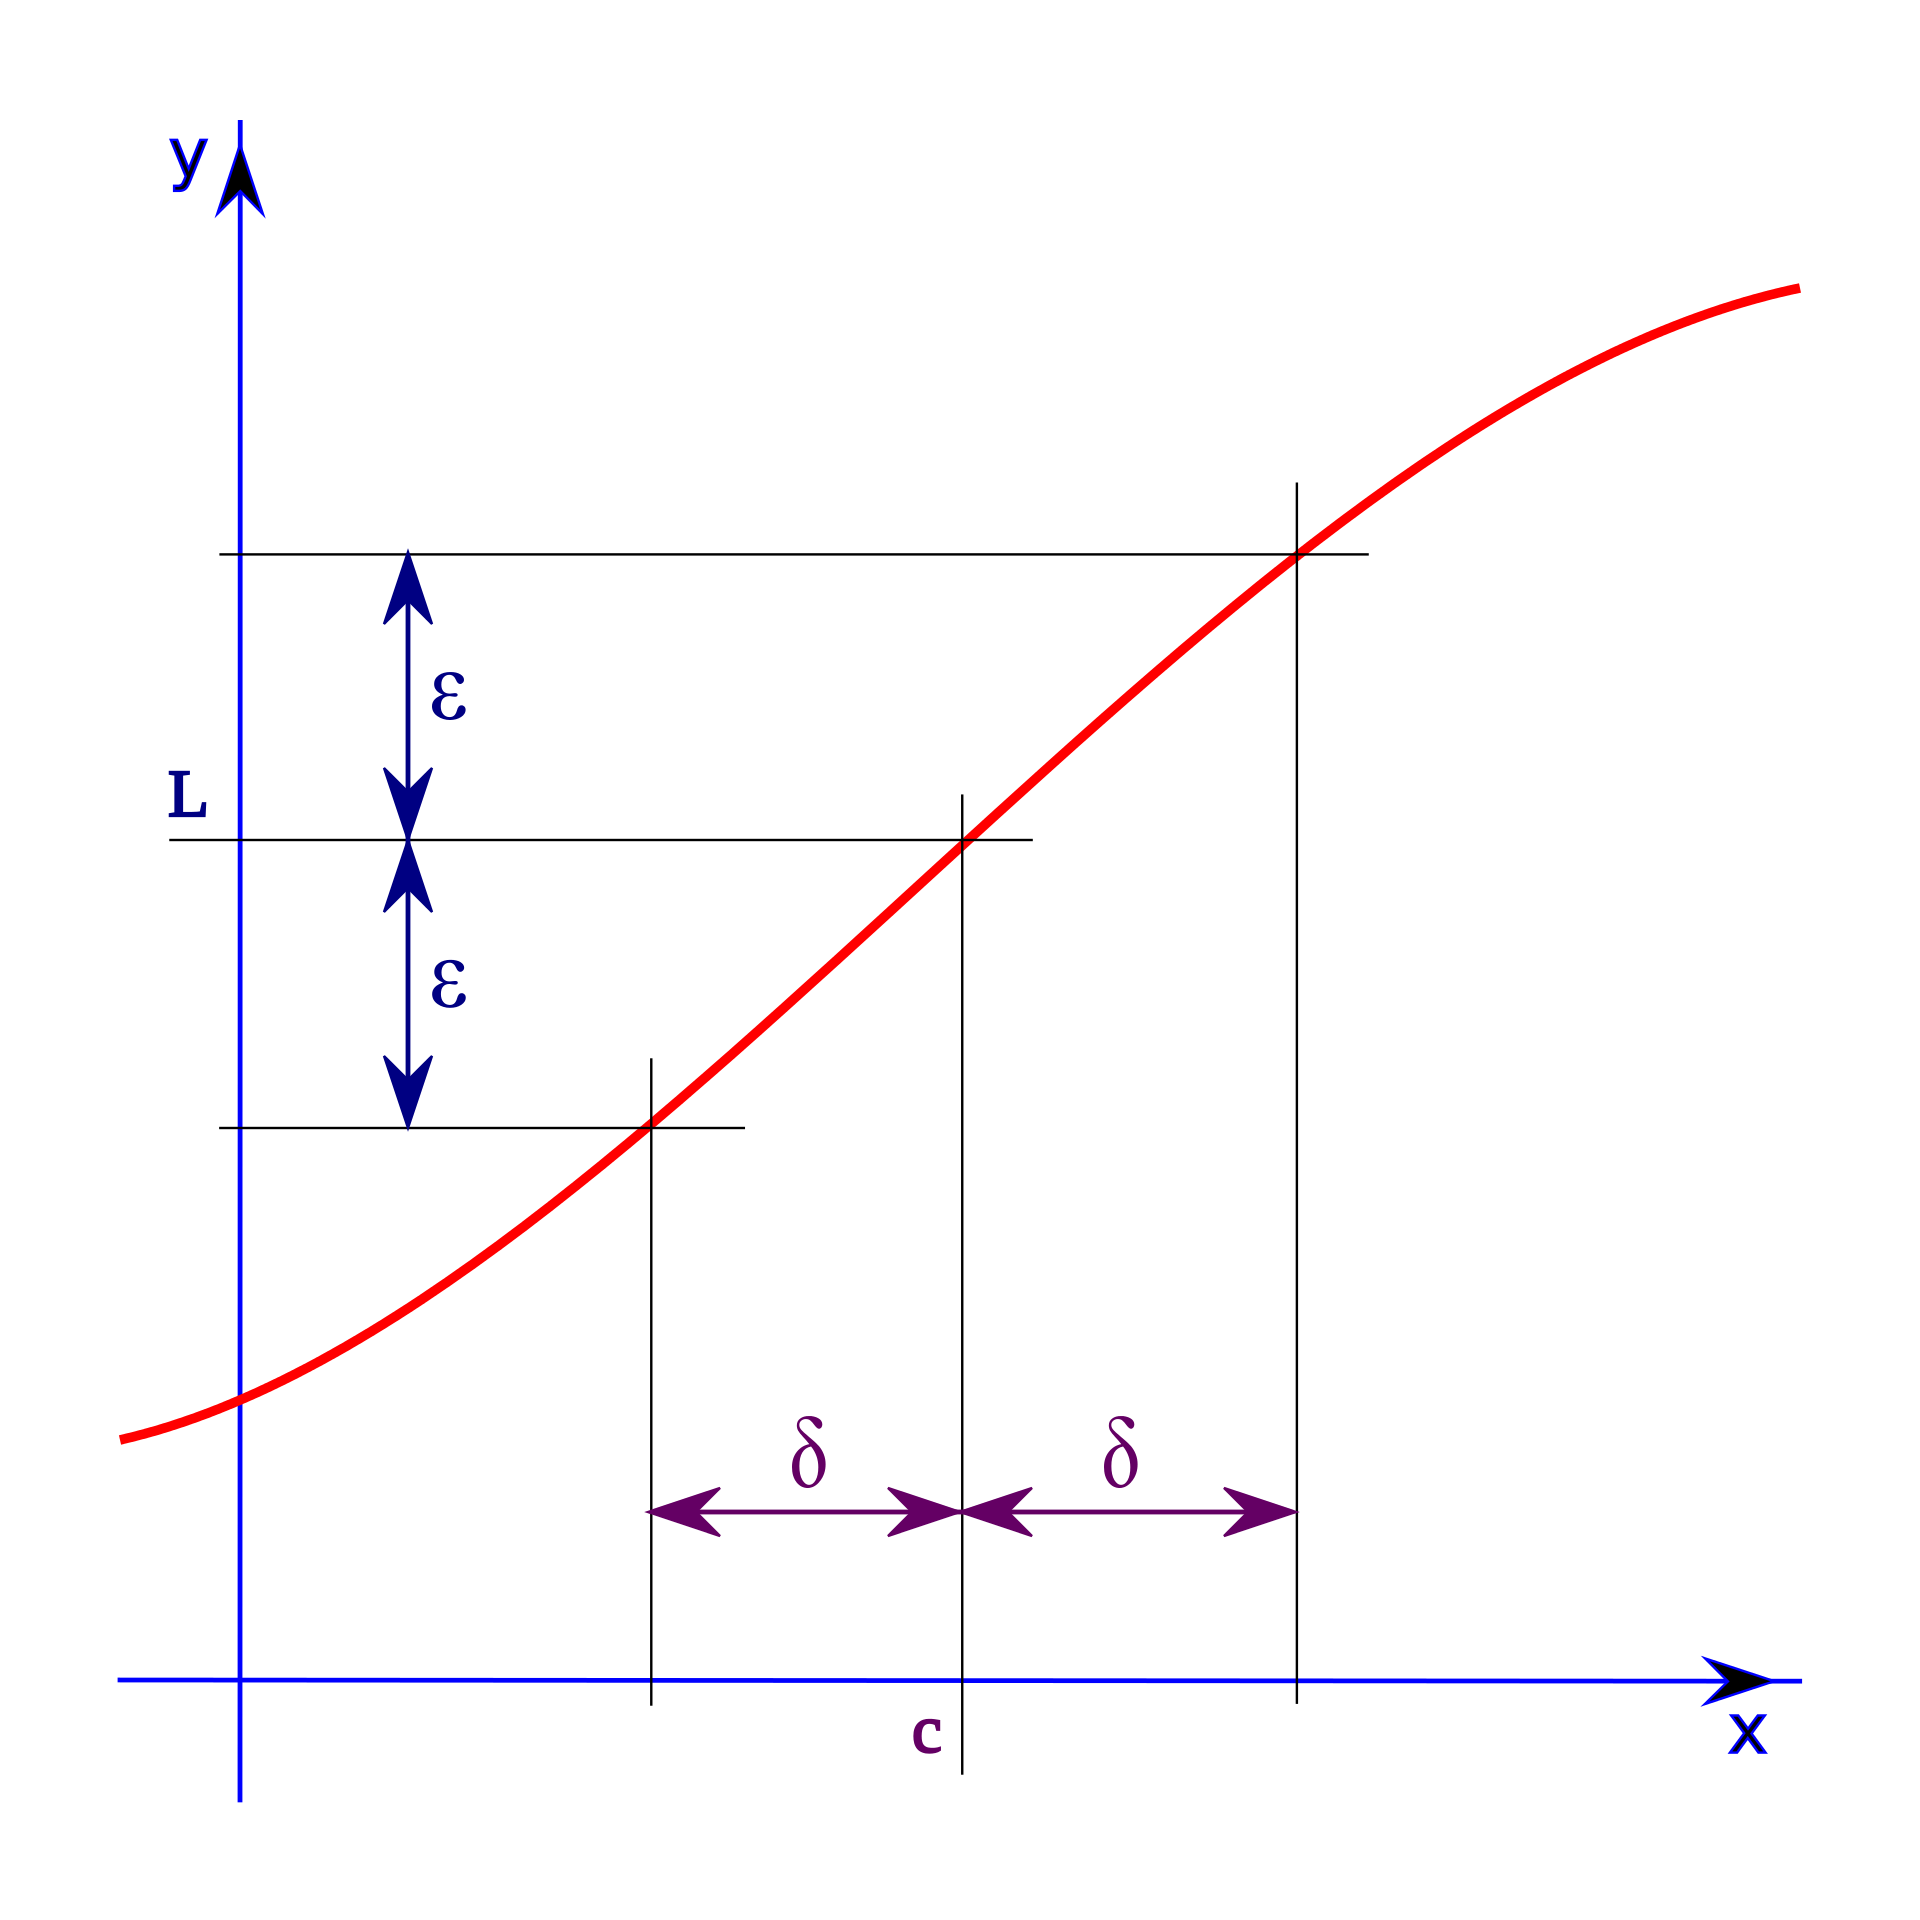
\includegraphics[width = 0.5\textwidth]{./limits_continuity/limit_epsilon_delta.png}
	\caption{\hyperref{https://en.wikipedia.org/wiki/(\%CE\%B5,\_\%CE\%B4)-definition\_of\_limit}{}{}{Wikipedia - $(\epsilon, \delta)\text{-definition of limit}$}}
\end{figure}
\noindent
Visually, what this means is that for any "error bound" of $y$ values $\epsilon$, I can give you a corresponding error bound of $x$ values $\delta$ such that all values of $f(z)$ for $z \in (c -\delta, c+ \delta)$ bound are between $L - \epsilon$ and $L + \epsilon$.

\noindent
We don't use this definition of the limit very often because it's a bit cumbersome.
However, it's important to know that when we use the limit, this is the formal definition making things work.

\begin{example}
	Use the $(\epsilon, \delta)$ definition of the limit to show that
	\begin{equation*}
		\lim_{x\to 0}{x\sin{\frac{1}{x}}} = 0.
	\end{equation*}
\end{example}
Letting $\epsilon > 0$, we need to find corresponding $\delta > 0$ that satisfies the definition for $L = 0$.
Knowing that $\sin$ is bounded between -1 and 1,
\begin{equation*}
	\abs{x\sin{\frac{1}{x}} - 0} = \abs{x\sin{\frac{1}{x}}} = \abs{x}\abs{\sin{\frac{1}{x}}} \leq \abs{x}.
\end{equation*}
\indent
Letting $\delta = \epsilon$, if $0 < \abs{x - 0} < delta$, then $\abs{x\sin{\frac{1}{x}} - 0} \leq \abs{x} < \epsilon$, as required by the definition.
\section{Limit Properties}
Limit have many nice properties all allow us to make useful simplifications when evaluating a limit.
Let
\begin{equation*}
	\lim_{x \to c}{f(x)} = L \text{ and } \lim_{x \to c}{g(x)} = M.
\end{equation*}
\begin{align*}
	\textbf{Sum and Difference Rule: }& \lim_{x\to c}{\left(f(x) \pm g(x)\right)} = L \pm M \\
	\textbf{Product Rule: }& \lim_{x\to c}{\left(f(x)g(x) \right)} = LM \\
	\textbf{Constant Multiple Rule: }& \lim_{x \to c}{k\cdot f(x)} = k \lim_{x \to c}{f(x)} = kL \\
	\textbf{Quotient Rule: }& \lim_{x \to c}{\frac{f(x)}{g(x)}} = \frac{\lim_{x \to x}{f(x)}}{\lim_{x \to c}{g(x)}} = \frac{L}{M} \text{, if} M \neq 0 \\
	\textbf{Power Rule: }& \text{If } n \neq  \in \R \text{, } \lim_{x\to c}{\left(f(x)\right)^n} = \left(\lim_{x \to c}{f(x)}\right)^n = L^n
\end{align*}

\subsection{``Substitution Rule''}
Although it may seem obvious from our idea that limits describe behavior at a point that if $f(x)$ is defined at $x=c$, then $\lim_{x\to c}{f(x)} = f(c)$.
However, this is \textit{not} always the case.
Remember that our definition of a limit required these $\epsilon$ and $\delta$ neighborhoods around the limit point.
If $f(x)$ is defined at $x=c$, but $(c, f(c))$ is not a point in these neighborhoods for any $\epsilon > 0$, then the limit will not evaluate to $f(c)$.

\begin{example}
	Find the limit of $f(x)$ as $x$ approaches $2$ for the following function.
	\begin{equation*}
		f(x) = \begin{cases}
			x^2 & x \neq 2 \\
			0 & x = 2
		\end{cases}.
	\end{equation*}
\end{example}
We can clearly see that $f(2) =  0$, but for $\epsilon = 0.1$ for example, there is no $\delta$ that can satisfy our definition, as points like $(2 - \delta, 4 - 2\delta + \delta^2)$ would outside the neighborhood around $(2,0)$.
In fact, the correct limit value is $4$, the same as if $f(x) = x^2$ for all $x$.
There are some more nuances we'll need to describe before we can say when it's OK to substitute to evaluate a limit.
\section{Left \& Right Hand Limits}
Our definition of the limit requires that the function get arbitrarily close to the limit value when approaching from both the left and right hand sides.
However, we can evaluate limits by specifying that we only approach from one side.
We usually notate this with a superscript $+$ or $-$ next to the $x$ limit value.
So,
\begin{equation*}
	\lim_{x \to 0^+}{f(x)}
\end{equation*}
would mean ``the limit of $f(x)$ as $x$ approaches $0$ from the right'', while
\begin{equation*}
	\lim_{x \to 0^-}{f(x)}
\end{equation*}
would mean ``the limit of $f(x)$ as $x$ approaches $0$ from the left.''

Our definition of the limit from both sides requires the left and right sides to be the same.
If they are different, the the limit does not exist.
\begin{align*}
	\lim_{x \to c^+}{f(x)} = \lim_{x \to c^-}{f(x)} &\implies \lim_{x \to c^+}{f(x)} = \lim_{x \to c^-}{f(x)} = \lim_{x \to c}{f(x)} \\
	\lim_{x \to c^+}{f(x)} \neq \lim_{x \to c^-}{f(x)} &\implies \lim_{x \to c}{f(x)} \text{ does not exist (DNE)}.
\end{align*}
\section{Sandwich Theorem}
We can use the Sandwich Theorem to indirectly find limits by "sandwiching" the function in question between two functions we do know the limit of.
If these two sandwiching functions go to the same value in the limit, then so to must the function in question.
\begin{theorem}[The Sandwich Theorem]
	If $g(x) \leq f(x) \leq h(x)$ and $\lim_{x \to c}{g(x)} = \lim_{x\to c}{h(x)} = L$, then $\lim_{x \to c}{f(x)} = L$.
\end{theorem}

\begin{example}
	Evaluate the following limit: $\lim_{x \to 0}{x\sin{\frac{1}{x}}}$.
\end{example}
We know that one of the properties of $\sin$ is that it oscillates between values of $-1$ and $-1$ for all input values.
So,
\begin{equation*}
	-1 \leq \sin{\frac{1}{x}} \leq 1.
\end{equation*}
\indent
Multiplying all terms by $x$,
\begin{equation*}
	-x \leq x\sin{\frac{1}{x}} \leq x.
\end{equation*}
\indent
Adding the limits,
\begin{equation*}
	\lim_{x\to 0}{-x} \leq \lim_{x \to 0}{x\sin{\frac{1}{x}}} \leq \lim_{x \to 0}{x}.
\end{equation*}
\indent
Evaluating the outer limits of the inequality,
\begin{equation*}
	0 \leq \lim_{x \to 0}{x\sin{\frac{1}{x}}} \leq 0
\end{equation*}
\indent
So, by the Sandwich Theorem,
\begin{equation*}
	\lim_{x \to 0}{x\sin{\frac{1}{x}}} = 0.
\end{equation*}
\section{Infinite Limits}
Although our limit definition works for finite values of $c$, it's also useful to think about what happens as $c$ goes to $\pm\infty$.
We'll need to add to our limit definition to incorporate infinite values, since it doesn't make sense to talk about neighborhoods at infinity.
\begin{definition}
	Let $f$ be a real-valued function defined on some subset $D \subseteq \R$ that contains arbitrarily large values.
	\begin{equation*}
		\lim_{x \to \infty}{f(x)} = L
	\end{equation*}
	if for every real $\epsilon > 0$, there is a real number $N > 0$ such that for all $x \in D$,
	\begin{equation}
		x > N \implies \abs{f(x) - L} < \epsilon.
	\end{equation}
\end{definition}

All the same properties that we described for finite limits, like the Sum and Difference Rule, still hold for infinite limits.

\subsection{End Behavior Model}
When x is numerically large, we can often model the behavior of a complicated function with a simplier one that behaves roughly the same for numerically large input values and is the same in the limit.
There are a few rules that these follow.
\begin{enumerate}
	\item For a polynomial, the end-behavior is highest-degree term.
	\item For a rational function, like a ratio of polynomials, the end behavior is the ratio of the highest degree terms.
	\item For more complicated functions, we may need to use some reasoning about the graph of the function and limit properties to determine end-behavior.
\end{enumerate}

\subsection{Horizontal Asymptotes}
Horizontal Asymptotes are a special type of end-behavior model.
\begin{definition}
	The line $y=b$ is a horizontal asymptote of $y = f(x)$ if $\lim_{x\to \infty}{f(x)} = b$ or $\lim_{x \to -\infty}{f(x)} = b$.
\end{definition}

We can determine horizontal asymptotes for rational functions (usually quotient of polynomials).
There are a few cases to consider
\begin{enumerate}
	\item If the numerator is a higher degree than the denominator, there is no horizontal asymptote, so we'll need a different method to calculate what happens at $\pm\infty$.
	\item If the denominator is a higher degree than the numerator, then there is a horizontal asymptote at $y = 0$.
	\item If the numerator and denominator have the same degree, there is a horizontal asymptote at $y = k$ where k is the ratio of the highest degree terms.
\end{enumerate}

\begin{example}
	Find the following limits, if they exist.\\
	\begin{table}[H]
	\begin{center}
	\begin{tabular}{ l l l}
		1. $\begin{aligned}[t]
			\lim_{x \to \infty}{\frac{x^3 - 6x + 1}{x^2 + 2x - 3}}
		\end{aligned}$ & 
		2. $\begin{aligned}[t]
			\lim_{x\to -\infty}{\frac{x-9}{2x-x^2}}
		\end{aligned}$ &
		3. $\begin{aligned}[t]
			\lim_{x\to \infty}{\frac{6x^2-4x^5+7x-1}{12x^5-3x^2+2}}
		\end{aligned}$ \\
		\hspace{1pt} & \hspace{1pt}\\
		4. $\begin{aligned}[t]
			\lim_{x\to \infty}{\frac{3x+1}{\abs{x}+2}}
		\end{aligned}$ &
		5. $\begin{aligned}[t]
			\lim_{x \to \infty}{x + e^{-x}}
		\end{aligned}$ &
		6. $\begin{aligned}[t]
			\lim_{x \to -\infty}{x + e^{-x}}
		\end{aligned}$
	\end{tabular}
	\end{center}
	\end{table}
\end{example}
\begin{answer}
	\begin{enumerate}
		\item Since the numerator degree is bigger than the denominator degree, we'll need to use the end behavior model.
			The end behavior model tells us that the numerator term dominates and has positive values, so the limit evaluates to $\infty$.
		\item Since the denominator has higher degree than the numerator, there is a HA at $y=0$, so the limit evaluates to $0$.
		\item Since the numerator and denominator have the same degree, the limit is the ratio of the highest-degree coefficients, $\frac{-1}{3}$.
		\item The numerator and denominator have the same degree. For $x > 0$, $\abs{x}+2 = x+2$, so the limit is the ratio of highest-degree coefficients, $3$.
		\item Looking at the two terms, we can see that as $x$ gets large, $e^{-x}$ gets very small, contributing less and less to the overall value.
			So, we can say that this function as a right end behavior model of $x$, so the limit is $\infty$.
		\item Looking at the two terms, we that that as $x$ gets very large and negative, $e^{-x}$ changes much faster than $x$.
			That is, $e^{-x}$ contributes more and more to the overall value of the function compared to $x$.
			So, we can say that this function has a left end behavior model of $e^{-x}$, so the limit is $\infty$.
	\end{enumerate}
\end{answer}
\section{Continuity Definition}
When we were looking at limits, we noticed that we can't always substitute to find the limit, even if the function is defined there.
In the example given to show that substitution and the limit can give different results, we saw a special type of function that seemed to have a ``hole'' at the point we were interested in finding the limit of.
This function is said to be discontinuous at this point, and in this section we'll define when a function is or isn't continuous at a point based on this idea of the limit and substitution giving different values.

\begin{definition}
	Let $f(x)$ be a real-valued function defined over $D \subseteq \R$.
	$f(x)$ is continuous at some point $x = c$ if all of the following hold.
	\begin{enumerate}
		\item $\lim_{x \to c}{f(x)}$ exists
		\item $f(c)$ is defined
		\item $\lim_{x \to c}{f(x)} = f(c)$ (substitution works)
	\end{enumerate}
	Otherwise, $f(x)$ is discontinuous at $c$.\footnote{Note that it's not necessary for $c \in D$.}
\end{definition}


We say that a function is continuous on an interval if it's continuous on every point in that interval.\footnote{If the interval is closed on one or both sides, we check continuity on the open interval. Then, we check the closed endpoints by looking at the limit from only one side.}

\begin{example}
	Find the points of continuity and discontinuity of the following functions
	\begin{table}[H]
	\begin{center}
	\begin{tabular}{ l l }
		1. $\begin{aligned}
			f(x) = \frac{1}{x^2+1}
		\end{aligned}$ &
		2. $\begin{aligned}
			g(x) = e^{1/x}
		\end{aligned}$
	\end{tabular}
	\end{center}
	\end{table}
\end{example}
\begin{answer}
	\begin{enumerate}
		\item There are no points where $f(x)$ or its limit are undefined.
			Further, there are no points where $f$ and its limit at that point are different.
			So, $f$ is continuous on $(-\infty, \infty)$ and discontinuous on $\emptyset$.
		\item Since $1/x$ is undefined at $x = 0$, $g(x)$ is also undefined at $x=0$.
			At every other point, $g$ and its limit are defined and are equal.
			So, $g$ is continuous on $(\infty, 0) \cup (0, \infty)$ and discontinuous on $[0]$.
	\end{enumerate}
\end{answer}
\section{Discontinuity Types}
There are four major types of discontinuity.
\begin{enumerate}[label=]
	\item \textbf{Removable: } If $f$ is discontinuous at $c$ but we can remove the discontinuity by setting $f$ equal to its limit at $c$, then $f$ has a removable discontinuity at $c$.
	\item \textbf{Jump: } If $f$ is discontinuous at $c$, and both of the one-sided limits exist but are different, then $f$ has a jump discontinuity at $c$.
	\item \textbf{Infinite: } If $f$ has a vertical asymptote at $c$, meaning one or both sides go to $\pm\infty$, then $f$ has an infinite discontinuity at $c$.
	\item \textbf{Oscillating: } If $f$ oscillates without limit at $c$, then $f$ has an oscillating discontinuity at $c$. An example of such a function would be $\sin{\frac{1}{x}}$ at $x=0$.
\end{enumerate}


It might seem strange that $\sin{\frac{1}{x}}$ has an oscillating discontinuity at $x=0$ because we were able to find the limit as $x$ approaches of 0 of $x\sin{\frac{1}{x}}$, a very similar function.
However, remembering how we applied the Ham Sandwich Theorem to find this limit, we see that the $x$ term bounds the amplitude of the oscillations, allowing the limit to be $0$.

\begin{example}
	For the following function state the following: its domain, any discontinuities and their types, what values should redefine the function to remove any removable discontinuities (give the extended function).
	\begin{equation*}
		f(x) = \frac{x^3-7x-6}{x^2-9}
	\end{equation*}
\end{example}
\begin{answer}
	Polynomials are continuous on their entire domain of all real numbers.
	So, rational functions like $f$ can only be discontinuous when the denominator is equal to $0$.
	This happens in two places: $x=3$ and $x=-3$.
	We'll check the limits from each side at each of these points to determine the type of discontinuity.
	For $x=3$,
	\begin{equation*}
		\lim_{x\to 3^+}{f(x)} = \lim_{x\to 3^-}{f(x)} = \lim_{x\to 3}{f(x)} = \lim_{x\to 3}{\frac{(x+2)(x+1)(x-3)}{(x+3)(x-3)}} = \lim_{x\to 3}{\frac{(x+2)(x+1)}{(x+3)}} = \frac{20}{6} = \frac{10}{3}.
	\end{equation*}
	
	So, $f$ has a removable discontinuity at $x=3$ because the left and right limits are the same.
	For $x=3$,
	\begin{equation*}
		\lim_{x\to -3^+}{f(x)} = -\infty \text{ and } \lim_{x\to -3^+}{f(x)} = \infty.
	\end{equation*}
	
	So, $f$ has an infinite discontinuity at $x=-3$ because both of the left and right limits go to $\pm\infty$.
	The value we got from the limits at $x=3$ gives us the value we need to redefine $f$ as to remove the discontinuity.
	The extended function is therefore
	\begin{equation*}
		f_{e}(x) = \begin{cases}
			f(x) & x \neq 3 \\
			\frac{10}{3} & x = 3
		\end{cases}
	\end{equation*}
\end{answer}
\section{Continuity Properties}
These properties should look very similar to the properties of limits.
Let $f$ and $g$ be continuous functions at $c$.
\begin{align*}
	\textbf{Sum and Difference Rule: }& f \pm g \text{ is continuous at } c. \\
	\textbf{Product Rule: }& f \cdot g \text{ is continuous at } c. \\
	\textbf{Constant Multiple Rule: }& kf \text{ is continous at } c \text{ for all real } k. \\
	\textbf{Quotient Rule: }& \frac{f}{g} \text{ is continuous at } c \text{ as long as the value of the extended function of } \\
		g \text{ at } c \text{ is not } 0. \\
	\textbf{Composition Rule: }& f \circ g \text{ is continuous at } c \text{ if } f \text{ is continuous at } g(c). \\
	\textbf{Absolute Value Rule: }& \abs{f} \text{ is continuous at } c.
\end{align*}

The following types of functions are continuous on their domains
\begin{itemize}
	\item Polynomials
	\item Rational functions, except where the denominator is 0
	\item Trigonometric functions where defined
\end{itemize}

\begin{example}
	Show that the following function is continuous.
	\begin{equation*}
		f(x) = \tan{\left(\frac{x^2}{x^2+4}\right)}.
	\end{equation*}
\end{example}
\begin{answer}
	We can write $f$ as the composition of $\tan{x}$ and $\frac{x^2}{x^2+4}$.
	$\tan{x}$ is continuous on its domain because it is a trigonometric function.
	The only points not in its domain are $(2n+1)\frac{\pi}{2}$, where $n$ is an integer.
	$\frac{x^2}{x^2+4}$ is a rational function, but it's denominator is never $0$, so it is continuous over all real numbers.
	Now, we just need to check that all points in the range of $\frac{x^2}{x^2+4}$ are in the domain of $\tan{x}$.
	The range of $\frac{x^2}{x^2+4}$ is $[0,1)$.
	None of the points in this interval are not in the domain of $\tan{x}$, so the composition is continuous over all real numbers.
\end{answer}
\section{Intermediate Value Theorem}
\begin{theorem}[Intermediate Value Theorem (IVT)]
	If $f$ is continuous on the closed interval $[a,b]$, then for all $c \in [f(a), f(b)]$, there exists $x \in [a,b]$ such that $f(x) = c$.
\end{theorem}

That is, if $f$ is continuous on $[a,b]$, then $f$ must take on every value between $f(a)$ and $f(b)$.
This encapsulates the idea that if a function is continuous on some interval, then it is ``connected'' on that interval.

\begin{example}
	Use the IVT to show that $e^{-x} = x$ has at least one solution.
\end{example}
\begin{answer}
	Let $f(x) = e^{-x} - x$.
	We are looking for $x$ where $f(x) = 0$.
	$f(0) = 1$ and $f(1) = \frac{1}{e} - 1$.
	Since $f$ is continuous on the closed interval $[0,1]$, it must take on every value between $1$ and $\frac{1}{e} - 1$.
	Since $1$ is positive and $\frac{1}{e} - 1$ is negative, 0 is between these two values.
	Thus, by the IVT, there must exist a solution between $x=0$ and $x=1$.
\end{answer}
		\chapter{Derivatives}
\noindent
Derivatives describe how a function is changing.
They are one of the two fundamental operations in calculus.

\section{Rates of Change \& Tangent Lines}
You might already be familiar from physics with the idea of an average rate of change over some interval (often a time interval in physics).
It is simply the amount of change that occurred in the interval, divided by the length of the interval.
This is exactly the same idea as the slope of a line being "rise over run"
\begin{equation*}
	\overline{\Delta f_{a,b}} = \frac{f(b)-f(a)}{b-a}.
\end{equation*}
This is also known as the ``secant slope'', which gets its name from secant lines on circles.

\begin{example}
	Find the average rate of change of $x^2-1$ over the interval $[1,4]$.
\end{example}
\begin{answer}
	Applying the formula,
	\begin{equation*}
		\overline{\Delta f_{1,4}} = \frac{f(4)-f(1)}{4-1} = \frac{15-0}{3} = 5.
	\end{equation*}
\end{answer}

As we decrease the size of the interval, the secant line becomes closer and closer to a tangent line.
In the limit, as the size of the interval approaches 0, we get a tangent line, representing an instantaneous rate of change.
\begin{equation*}
	\Delta f_a = \lim_{h \to 0}{\frac{f(a+h)-f(a)}{h}}.\footnote{You may recognize this from pre-calculus as the ``difference quotient''.}
\end{equation*}

\begin{figure}[H]
	\label{sectant_tangent_line}
	\centering
	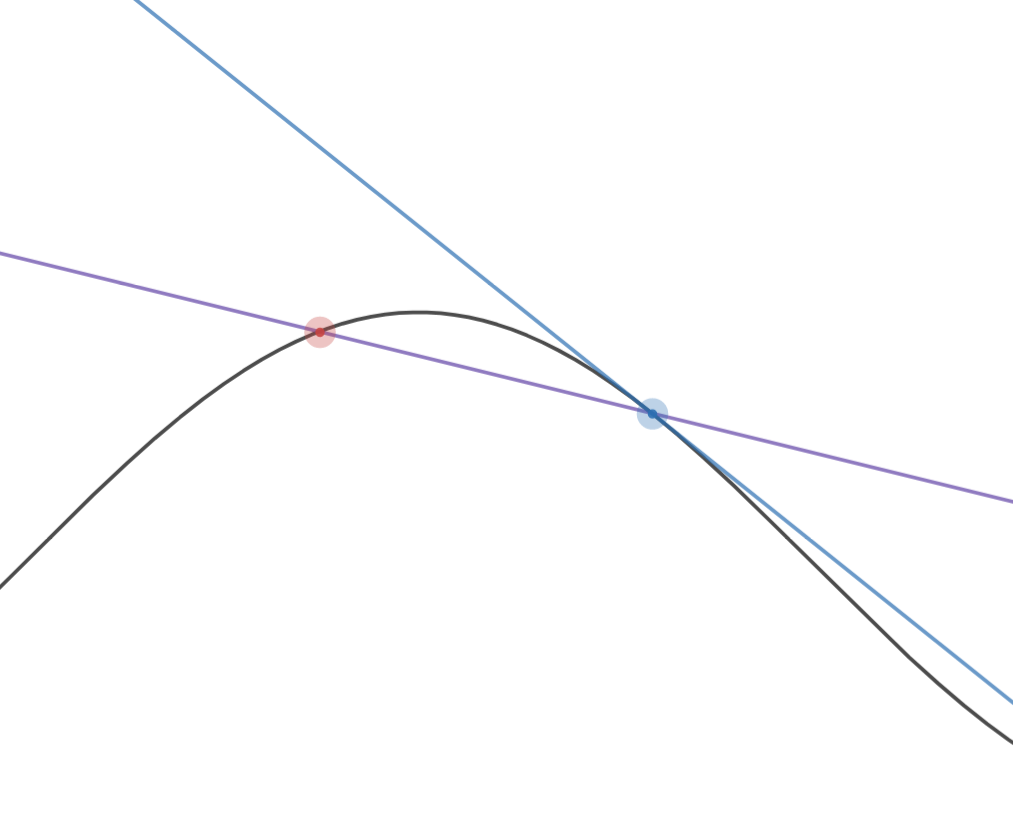
\includegraphics[width = 0.5\textwidth]{./derivatives/secant_tangent_line.png}
	\caption{\hyperref{}{}{}{Secant and Tangent Line}}
\end{figure}

\begin{example}
	Find the equation of the tangent line to $f(x)=x^2-4x$ at $x=1$.
\end{example}
\begin{answer}
	First, we need to find the instantaneous rate of change of $f$ at $x=1$.
	We do this by evaluating the limit.
	\begin{align*}
		\Delta f_{1} &= \lim_{h \to 0}{\frac{f(1+h)-f(1)}{h}} \\
		&= \lim_{h \to 0}{\frac{(1+h)^2-3(1+h) - (1)^2 + 3(1)}{h}} \\
		&= \lim_{h \to 0}{\frac{h^2 + 2h + 1 - 3 - 3h - 1 + 3}{h}} \\
		&= \lim_{h \to 0}{\frac{h^2 - h}{h}} \\
		&= \lim_{h \to 0}{h - 1} \\
		&= -1.
	\end{align*}
	
	Now that we have the slope of the tangent line, we can write the equation of the line in point-slope form.
	We can also rearrange to standard for is needed.
	\begin{align*}
		y - f(1) &= -1(x - 1) \\
		y + 2 &= -x + 1 \\
		y &= -x - 1.
	\end{align*}
\end{answer}
\section{Definition of the Derivative}
\begin{definition}
	The derivative of a function $f(x)$, notated $f^\prime(x)$, is the slope of $f$ at any point along $f$.
	This is also the slope of the tangent line to $f$ at this point, which is also the instantaneous rate of change of $f$ at this point.
	\begin{equation}
		f^\prime(x) = \lim_{h \to 0}{\frac{f(x+h)-f(x)}{h}} \text{ (assuming the limit exists).}
	\end{equation}
\end{definition}

\begin{example}
	Find the derivative of $f(x)=x^2+4$.
\end{example}
\begin{answer}
	Applying the definition,
	\begin{align*}
		f^\prime(x) &= \lim_{h\to 0}{\frac{f(x+h)-f(x)}{h}} \\
		&= \lim_{h \to 0}{\frac{(x+h)^2+4 - x^2 - 4}{h}} \\
		&= \lim_{h \to 0}{\frac{x^2 + 2xh + h^2 + 4 - x^2 - 4}{h}} \\
		&= \lim_{h \to 0}{\frac{2xh + h^2}{h}} \\
		&= \lim_{h\to 0}{2x + h} \\
		&= 2x.\footnotemark
	\end{align*}
\end{answer}
\footnotetext{Note that the constant term 4 didn't contribute anything to the outcome. It was canceled immediately when subtracting $f(x)$.}


There are a couple different notations that all mean the derivative of $y = f(x)$.
You should be familiar with all of them.
\begin{table}[H]
\begin{center}
\begin{tabular}{ l l l }
	$\begin{aligned}y^\prime\end{aligned}$ & & $\begin{aligned}\dd{y}{x}\end{aligned}$ \\
	& & \\
	$\begin{aligned}\dd{f}{x}\end{aligned}$ & & $\begin{aligned}\dd{}{x}f(x)\end{aligned}$
\end{tabular}
\end{center}
\end{table}

\subsection{Derivative at a Point}
The formula given in the definition is useful because it gives a function that can give the derivative at any point, but it may not be useful or feasible to use this formula.
Instead, we can use a formula to just give us the derivative at one point.
\begin{equation}
	f^\prime(a) = \lim_{x \to a}{\frac{f(x)-f(a)}{x-a}}.
\end{equation}

\begin{example}
	Find the derivative of $f(x) = \frac{1}{x}$ at $x=2$.
\end{example}
\begin{answer}
	Applying the formula for the derivative at a point,
	\begin{align*}
		f^\prime(2) &= \lim_{x \to 2}{\frac{f(x)-f(2)}{x-2}} \\
		&= \lim_{x \to 2}{\frac{1/x - 1/2}{x-2}} \\
		& = \lim_{x \to 2}{\frac{-(x-2)}{2x(x-2)}} \\
		&= \lim_{x \to 2}{\frac{-1}{2x}} \\
		&= \frac{-1}{4}.
	\end{align*}
\end{answer}

\subsection{Left \& Right Hand Derivatives}
The normal derivative is defined in terms of a two-sided limit, meaning that the left and right hand limits are equal.
However, we can also calculate left and right hand derivatives at every point along the function's domain, which may be useful if the left and right hand derivatives are not equal or the point in question is on the boundary of the domain.

\begin{example}
	Find the left and high hand derivatives of the following function at $x=1$.
	Say if the derivative at this point exists and why.
	\begin{equation*}
		f(x) = \begin{cases}
			x^2 + x & x \leq 1 \\
			x+1 & x > 1
		\end{cases}.
	\end{equation*}
\end{example}
\begin{answer}
	Evaluating the left hand limit,
	\begin{align*}
		f^\prime(1^-) &= \lim_{x \to 1^-}{\frac{f(x)-f(1)}{x-1}} \\
		&= \lim_{x \to 1^-}{\frac{x^2 + x - 2}{x-1}} \\
		&= \lim_{x \to 1^-}{\frac{(x-1)(x+2)}{x-1}} \\
		&= \lim_{x \to 1^-}{x+2} \\
		&= 3.
	\end{align*}
	
	Evaluating the right hand limit,
	\begin{align*}
		f^\prime(1^+) &= \lim_{x \to 1^+}{\frac{f(x)-f(1)}{x-1}} \\
		&= \lim_{x \to 1^+}{\frac{x + 1 - 2}{x-1}} \\
		&= \lim_{x \to 1^+}{\frac{x-1}{x-1}} \\
		&= 1.
	\end{align*}
	
	Since $f^\prime(1^-) \neq f^\prime(1^+)$, the derivative does not exist at $x=1$.
\end{answer}
\section{Differentiability}
As we saw when looking at left and right hand derivatives, a derivative will fail to exist when the left and right hand derivatives differ.
However, there are several other cases where a function might not be differentiable at a point.
\begin{enumerate}
	\item \textbf{Corner: } This is the simplest case where both the one sided derivatives exist, are finite, but are different.
		An example would be $f(x)=\abs{x}$ at $x=0$.
	\item \textbf{Cusp: } This is sort of an extreme example of a corner where the one of the one sides derivatives approaches $-\infty$ and the other approaches $\infty$.
		An example would be $f(x)=\sqrt[3]{x^2}$ at $x=0$.
	\item \textbf{Vertical Tangent: } This is where the one sided derivatives exist and agree, but approach $-\infty$ or $\infty$.
		An example would be $f(x)=\sqrt[3]{x}$ at $x = 0$.
	\item \textbf{Discontinuity: } This is where one of the one sided derivatives doesn't exist.
		An example would be the unit step function at $x=0$, which is 1 for $x \geq 0$ and -1 for $x < 0$.
\end{enumerate}

\subsection{Differentiability Implies Local Linearity}
A function is locally linear at a point $a$ when it is differentiable at $a$ and closely resembles its own tangent line at $a$.
Visually, what this means is that as you "zoom in" on a locally linear point, the curve will look more and more like a line.

\begin{figure}[H]
	\label{locally_linear}
	\centering
	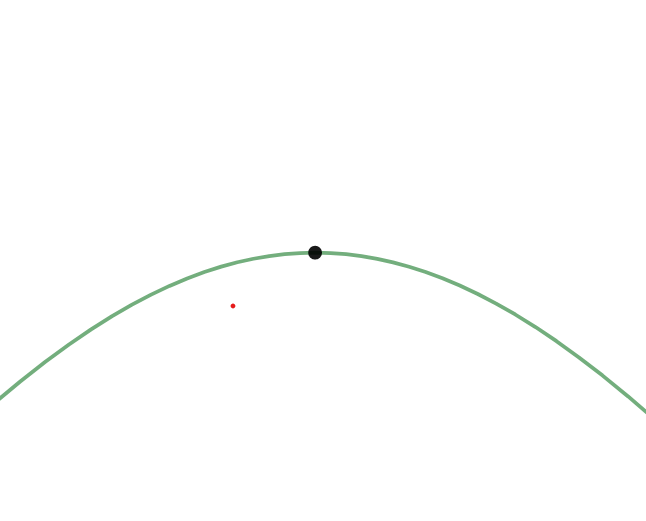
\includegraphics[width = 0.25\textwidth]{./derivatives/cos1.png}
	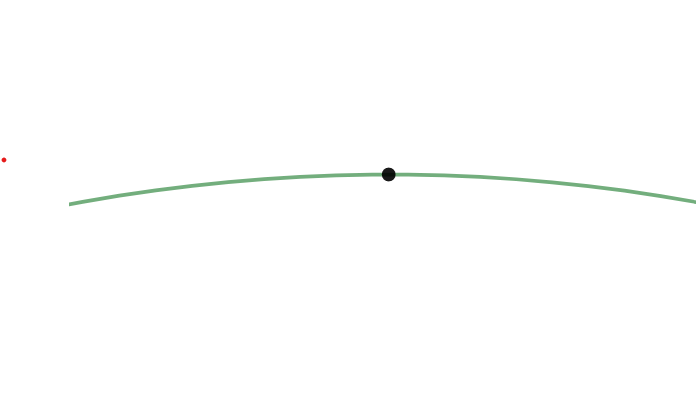
\includegraphics[width = 0.25\textwidth]{./derivatives/cos2.png}
	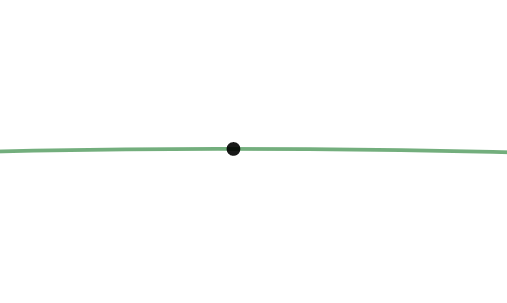
\includegraphics[width = 0.25\textwidth]{./derivatives/cos3.png}
	\caption{\hyperref{}{}{}{Zooming in on a $\cos$ curve}}
\end{figure}

\subsubsection{Numerical Approximation: Symmetric Difference Quotient}
We can use the derivative at a point and a very small value of $h$ to approximate the tangent slope.
However, we can get a better estimate with the same value of $h$ by using the symmetric difference quotient.
\begin{equation*}
	\frac{f(a+h)-f(a-h)}{2h}.
\end{equation*}

A calculator might prefer this formula because it tends to give better approximations.

\subsection{Differentiability Implies Continuity}
\begin{theorem}
	If $f^\prime(a)$ exists, then $f$ is continuous at $a$.
\end{theorem}

The converse is not necessarily true: a function can be continuous but not differentiable.

\begin{example}
	Determine whether or not the follow function is differentiable at $x=2$.
	\begin{equation*}
		f(x) = \begin{cases}
			x^2 + 1 & x \leq 2 \\
			4x-4 & x > 2
		\end{cases}.
	\end{equation*}
\end{example}
\begin{answer}
	Looking at the graph of this function, we see there is a jump discontinuity at $x=2$.
	If the function was differentiable at $x=2$, it would be continuous at $x=2$.
	Since it is not continuous at $x=2$, it must not be differentiable at $x=2$.
\end{answer}
\section{Intermediate Value Theorem for Derivatives}
\begin{theorem}[IVT for Derivatives]
	If $f$ is differentiable on the closed interval $[a,b]$, then $f^\prime$ takes on every value between $f^\prime(a)$ and $f^\prime(b)$.
\end{theorem}

\begin{example}
	Show that any function that has the following function as it derivative cannot be differentiable on the interval $-1 \leq x \leq 1$.
	\begin{equation*}
		f(x) = \begin{cases}
			0 & -1 \leq x < 0 \\
			1 & 0 \leq x \leq 1
		\end{cases}.
	\end{equation*}
\end{example}
$f$ does not take all values between $f(-1)=0$ and $f(1)=1$.
So, by the contrapositive of the IVT for Derivatives, any function that has $f$ as its derivative will not be differentiable on $[-1,1]$.
\section{Derivative Rules}

\subsection{Basic Properties}
All of these properties should look familiar from properties of limits and continuity.
Let $f$ and $g$ be differentiable functions of $x$.
Let $c$ be some real constant.
\begin{align*}
	\textbf{Sum and Difference Rule: }& (f \pm g)^\prime = f^\prime \pm g^\prime \\
	\textbf{Constant Multiple Rule: }& (cf)^\prime = cf^\prime \\
	\textbf{Constant Rule: }& (c)^\prime = 0
\end{align*}
\footnotetext{This follows from using the sum and difference rule with the power rule.}

\subsection{Power Rule}
\begin{lemma}
	Let $f(x) = x^n$ where $n$ is a positive integer. Then
	\begin{equation}
		f^\prime(x) = nx^{n-1}.
	\end{equation}
\end{lemma}
\begin{proof}
	Applying the limit definition of the derivative,
	\begin{equation*}
		f^\prime(x) = \lim_{h \to 0}{\frac{(x+h)^n - x^n}{h}}.
	\end{equation*}
	Applying the binomial theorem (think Pascal's Triangle),
	\begin{align*}
		f^\prime(x) &= \lim_{h \to 0}{\frac{x^n + nhx^{n-1} + \ldots + {n \choose k}h^{k}x^{n-k} + \ldots + h^n - x^n}{h}} \\
		&= \lim_{h \to 0}{nx^{n-1} + \ldots + {n \choose k}h^{k-1}x^{n-k} + \ldots + h^{n-1}} \\
		&= nx^{n-1}.
	\end{align*}
\end{proof}
\noindent
We'll revisit the power rule after we discover some more detailed rules to show that $n$ can be any real number, not just a positive integer.
\subsection{Higher Order Derivatives}
\begin{definition}
	Let $n$ be a positive integer. The $n^{th}$ derivative of $f$ is
	\begin{equation*}
		f^{(n)}(x) = \dd{}{x}{f^{(n-1)}}(x),
	\end{equation*}
	where $f^{(n-1)}(x)$ is the ${n-1}^{th}$ derivative of $f$.
	Using equivalent notation,
	\begin{equation*}
		\dd{{}^n}{x^n}f = \dd{{}^{n-1}}{x^{n-1}}f.
	\end{equation*}
\end{definition}

\begin{example}
	Find the third derivative of $f(x) = x^3 + x^2$.
\end{example}
Taking the derivative once using the power rule and sum and difference rule,
\begin{equation*}
	f^\prime(x) = 3x^2 + 2x.
\end{equation*}
\indent
Taking the derivative a second time using the power, constant multiple rules, and sum and difference rules,
\begin{equation*}
	f^{\prime\prime}(x) = 6x + 2.
\end{equation*}
\indent
Taking the derivative a final time using the power, constant multiple, constant, and sum and difference rules,
\begin{equation*}
	f^{\prime\prime\prime}(x) = 6.
\end{equation*}
\subsection{Product Rule}
\begin{lemma}
	Let $f$ and $g$ be differentiable functions. Then
	\begin{equation}
		(fg)^\prime = fg^\prime + gf^\prime.
	\end{equation}
\end{lemma}
\begin{proof}
	Applying the definition of the derivative and limit properties,
	\begin{align*}
		(fg)^\prime &= \lim_{h \to 0}{\frac{f(x+h)g(x+h) - f(x)g(x)}{h}} \\
		&= \lim_{h \to 0}{\frac{f(x+h)g(x+h)-f(x+h)g(x)+f(x+h)g(x)-f(x)g(x)}{h}} \\
		&= \lim_{h \to 0}{\frac{f(x+h)\left(g(x+h)-g(x)\right)}{h}} + \lim_{h \to 0}{\frac{g(x)\left(f(x+h)-f(x)\right)}{h}} \\
		&= \lim_{h \to 0}{f(x+h)} \lim_{h \to 0}{\frac{g(x+h)-g(x)}{h}} + g(x)\lim_{h \to 0}{\frac{f(x+h)-f(x)}{h}} \\
		&= fg^\prime + gf^\prime
	\end{align*}.
\end{proof}

\begin{example}
	Given the the derivative of $\sin{(x)}$ is $\cos{(x)}$, find the derivative of $x^2\sin{(x)}$.
\end{example}
Using the product rule and power rule,
\begin{equation*}
	f^\prime(x) = x^2\cos{(x)} + \sin{(x)}2x.
\end{equation*}
\subsection{Quotient Rule}
\begin{lemma}
	Let $f$ and $g$ be differentiable functions where $g \neq 0$. Then
	\begin{equation}
		\left(\frac{f}{g}\right)^\prime = \frac{gf^\prime - fg^\prime}{g^2}.
	\end{equation}
\end{lemma}
\begin{proof}
	Using the definition of the derivative and limit properties,
	\begin{align*}
		\left(\frac{f}{g}\right)^\prime &= \lim_{h\to 0}{\frac{\frac{f(x+h)}{g(x+h)} - \frac{f(x)}{g(x)}}{h}} \\
		&= \lim_{h\to 0}{\frac{1}{h}\frac{f(x+h)g(x) - f(x)g(x+h)}{g(x+h)g(x)}} \\
		&= \lim_{h\to 0}{\frac{1}{h}\hspace{3pt}\frac{f(x+h)g(x) - f(x)g(x) + f(x)g(x) - f(x)g(x+h)}{g(x+h)g(x)}} \\
		&= \lim_{h \to 0}{\frac{1}{g(x+h)g(x)}\hspace{3pt}\frac{f(x+h)g(x)-f(x)g(x)+f(x)g(x)-f(x)g(x+h)}{h}} \\
		&= \lim_{h \to 0}{\frac{1}{g(x+h)g(x)}\left(\frac{f(x+h)g(x)-f(x)g(x)}{h}+\frac{f(x)g(x)-f(x)g(x+h)}{h}\right)} \\
		&= \lim_{h \to 0}{\frac{1}{g(x+h)g(x)}} \left(g(x)\lim_{h \to 0}{\frac{f(x+h)-f(x)}{h}} - f(x)\lim_{h\to 0}{\frac{g(x+h)-g(x)}{h}}\right) \\
		&= \frac{1}{g^2(x)}\left(g(x)f^\prime(x) - f(x)g^\prime(x)\right) \\
		&= \frac{gf^\prime - fg^\prime}{g^2}.
	\end{align*}
\end{proof}

\begin{example}
	Given that the derivative of $\sin{(x)}$ is $\cos{(x)}$, find the derivative of $\frac{\sin{(x)}}{x^2}$.
\end{example}
Applying the quotient and power rules,
\begin{equation*}
	f^\prime(x) = \frac{x^2\cos{(x) - 2x\sin{(x)}}}{x^4} = \frac{x\cos{(x)}-2\sin{(x)}}{x^3}.
\end{equation*}
\subsection{Chain Rule}
\begin{lemma}
	Let $f$ and $g$ be differentiable functions. Then
	\begin{equation}
		\dd{}{x}f(g(x)) = f^\prime(g(x))g^\prime(x).
	\end{equation}
	Equivalently, if $f$ is a function of $g$ and $g$ is a function of $x$,
	\begin{equation}
		\dd{f}{x} = \dd{f}{g}\hspace{3pt}\dd{g}{x}.
	\end{equation}
\end{lemma}
\begin{proof}
	Applying the limit definitions of the derivative,
	\begin{align*}
		\dd{f}{x} &= \lim_{h \to 0}{\frac{f(g(x+h))-f(g(x))}{h}} \\
		&= \lim_{h\to 0}{\frac{f(g(x+h))-f(g(x))}{g(x+h)-g(x)}\hspace{3pt}\frac{g(x+h)-g(x)}{h}} \\
		&= \lim_{h\to 0}{\frac{f(g(x+h))-f(g(x))}{g(x+h)-g(x)}} \hspace{3pt} \lim_{h\to 0}{\frac{g(x+h)-g(x)}{h}} \\
		&= \left(\lim_{h\to 0}{\frac{f(g(x+h))-f(g(x))}{g(x+h)-g(x)}}\right) \hspace{3pt} \dd{g}{x} \\
		&= \dd{f}{g}\hspace{3pt}\dd{g}{x}.
	\end{align*}
\end{proof}

\begin{example}
	Find the derivative of $y = (x^2 + 1)^5$ using the chain rule.
\end{example}
$y$ is a composition of the two functions $x^5$ and $x^2 + 1$.
Applying the chain rule, 
\begin{equation*}
	y^\prime = \dd{}{(x^2+1)}(x^2+1)^5 \hspace{3pt} \dd{}{x}(x^2+1)
\end{equation*}
\indent
Making the substitution $u = x^2 + 1$,
\begin{align*}
	y^\prime &= \dd{}{u}u^5 \hspace{3pt} \dd{}{x}(x^2+1) \\
	&= 5u^{4}2x
\end{align*}
\indent
Substituting back,
\begin{align*}
	y^\prime &= 5(x^2+1)^{4}2x \\
	&= 10x(x^2+1)^4.
\end{align*}

\subsubsection{$u$ Substitutions}
As we did in the example, we can substitute a variable, usually called $u$ when applying the chain rule.
\begin{example}
	Given that the derivative of $\sin{x}$ is $\cos{x}$, find the derivative of $f(x)=\sin^5{x}$.
\end{example}
$f$ is a composition of $x^5$ and $\sin$.
Substituting $u=\sin{x}$, we can rewrite $f$ as $u^5$.
Applying the chain rule,
\begin{align*}
	\dd{f}{x} &= \dd{f}{u} \hspace{3pt} \dd{u}{x} \\
	&= 5u^4 \hspace{3pt} \cos{x} \\
	&= 5\sin^4{x}\cos{x}.
\end{align*}
\subsection{Exponential Rule}
Let's find the derivative of the most natural exponential function: $f(x) = e^x$.
Using the limit definition of the derivative,
\begin{align*}
	f^\prime(x) &= \lim_{h \to 0}{\frac{e^{x+h}-e^x}{h}} \\
	&= \lim_{h \to 0}{\frac{e^x\left(e^h - 1\right)}{h}} \\
	&= e^x \lim_{h \to 0}{\frac{e^h - 1}{h}}
\end{align*}
Remembering the following definition of $e$,
\begin{equation*}
	e = \lim_{n \to \infty}{\left(1+\frac{1}{n}\right)^n}.
\end{equation*}
Substituting $h = 1/n$,
\begin{equation*}
	e = \lim_{h \to 0}{\left(1+h\right)^{1/h}}.
\end{equation*}
Putting substituting this definition for $e$ into our work,
\begin{align*}
	f^\prime(x) &= e^x \lim_{h \to 0}{\frac{\left(\left(1+h\right)^{1/h}\right)^h-1}{h}} \\
	&= e^x \lim_{h \to 0}{\frac{\left(1+h\right)-1}{h}} \\
	&= e^x \lim_{h \to 0}{\frac{h}{h}} \\
	&= e^x.
\end{align*}
Amazingly, this function is equal to it's own derivative. In fact, aside from the trivial example of $0$, $e^x$ is the only function with this property. \\


We can apply the chain rule to find the derivative of $b^x$ for real, positive values of $b$.
\begin{equation*}
	f(x) = b^x	= e^{x\ln{b}}.
\end{equation*}
Let $u(x) = x\ln{b}$.
\begin{equation*}
	f(x) = b^x = e^{u(x)}.
\end{equation*}
Applying the chain rule,
\begin{align*}
	f^\prime(x) &= \dd{}{u}e^u \hspace{3pt} \dd{}{x}x\ln{b}. \\
	&= e^u \ln{b} \\
	&= e^{x\ln{b}} \ln{b} \\
	&= b^x \ln{b}.
\end{align*}

\begin{example}
	Find the derivative of $f(x) = 2^{x^2}$.
\end{example}
\begin{answer}
	Let $u(x) = x^2$.
	\begin{equation*}
		f(x) = e^u(x).
	\end{equation*}
	Using the exponential and chain rules,
	\begin{align*}
		f^\prime(x) &= \dd{f}{u} \hspace{3pt} \dd{u}{x} \\
		&= \dd{}{u}e^u \hspace{3pt} \dd{}{x}x^2 \\
		&= 2^u \ln{(2)} 2x \\
		&= 2^{x^2} \ln{(2)} 2x \\
		&=  2x\ln{(2)}2^{x^2}.
	\end{align*}
\end{answer}
\subsection{Implicit Differentiation}
Although we normally have equations of the form $y = f(x)$, some equations might be given in are are more convenient to write in different forms.
Using our understanding of the chain rule, we can still work with these forms and find $y^\prime$. There are generally three steps to finding $y^\prime$ when equations are given in these different forms.
\begin{enumerate}
	\item Get all terms involving $y$ to one side of the equation. This step is technically optional but usually makes the step 3 more convenient.
	\item Take the derivatives of both sides of the equation, using the chain rule.
	\item Rearrange to solve for $y^\prime$, making substitutions for $y$ to get the answer in terms of input parameters (e.g $x$).
\end{enumerate}
It's possible that you can get multiple solutions for $y^\prime$.
You'll need to check if 

\begin{example}
	Given that $y^2 = x$, find $y^\prime$ using implicit differentiation.
\end{example}
\begin{answer}
	Step 1 is already complete by what's given.
	Taking the derivative of both sides, remembering to use the chain rule,
	\begin{equation*}
		2yy^\prime = 1.
	\end{equation*}
	
	Solving for $y^\prime$,
	\begin{equation*}
		y^\prime = \frac{1}{2y}.
	\end{equation*}
	
	Looking back at our original equation, we see $y = \pm\sqrt{x}$.
	Substituting back into our work,
	\begin{equation*}
		y^\prime = \pm\frac{1}{2\sqrt{x}}.
	\end{equation*}
\end{answer}

Sometimes, it's not possible or is not necessary for what you're working on to complete step 3, meaning you leave your answer for $y^\prime$ in terms of $y$ and input parameters.
\begin{example}
	Find the derivative for $y$ with respect to $x$ at $(1,1)$ if $y^4 = x^3 + x + y$.
\end{example}
\begin{answer}
	Rearranging to complete step 1,
	\begin{equation*}
		y^4 - y = x^3 + x.
	\end{equation*}
	
	Taking the derivative of both sides,
	\begin{equation*}
		(4y^3 - 1)y^\prime = 3x^2 + 1.
	\end{equation*}
	
	Solving for $y^\prime$ and completing step 2,
	\begin{equation*}
		y^\prime = \frac{3x^2 + 1}{4y^3 - 1}.
	\end{equation*}
	
	Since we have both the $x$ and $y$ coordinates of where we're looking for the slope, we don't need to complete step 3.
	We can simply substitute to find our numerical answer for $y^\prime$.
	\begin{equation*}
		y^\prime_{(1,1)} = \frac{3 + 1}{4 - 1} = \frac{4}{3}.
	\end{equation*}
\end{answer}

Sometimes, we might already be given a formula for $y$, but rearranging and then doing implicit differentiation is easier.
\begin{example}
	Find the derivative with respect to $x$ of $y = \ln{x}$.
\end{example}
\begin{answer}
	We don't have any way to find the derivative of $\ln$ directly, but we do know how $\ln$ relates to exponential functions, a form we do know how to differentiate.
	Exponentiating both sides with base $e$,
	\begin{equation*}
		e^y = e^{\ln{x}} = x.
	\end{equation*}
	 
	Implicitly differentiating,
	\begin{equation*}
		e^{y}y^\prime = 1.
	\end{equation*}
	
	Solving for $y^\prime$,
	\begin{equation*}
		y^\prime = \frac{1}{e^y}.
	\end{equation*}
	
	Substituting what we were given for $y$,
	\begin{equation*}
		y^\prime = \frac{1}{e^{\ln{x}}} = \frac{1}{x}.
	\end{equation*}
\end{answer}

\subsubsection{Logarithmic Differentiation}
Logarithmic differentiation is a certain type of differentiation where you take to natural log of both sides and then implicitly differentiate.
It's especially useful when input parameters appear in both the base and exponent.
\begin{example}
	Find the derivative with respect to $x$ of $y = x^{\ln{x}}$.
\end{example}
\begin{answer}
	Taking the natural log of both sides,
	\begin{equation*}
		\ln{y} = \ln^2{x}.
	\end{equation*}
	
	Implicitly differentiating,
	\begin{align*}
		\frac{1}{y}y^\prime &= \frac{2\ln{x}}{x} \\
		y^\prime &= y\frac{2\ln{x}}{x} \\
		&= x^{\ln{x}}\frac{2\ln{x}}{x}.
	\end{align*}
\end{answer}


We now have the tools to prove the power rule for all real exponents.
\begin{proof}
	Let $n$ be an real number.
	\begin{align*}
		y &= x^n \\
		\ln{y} &= n\ln{x} \\
		\frac{1}{y}y^\prime &= n\frac{1}{x} \\
		y^\prime &= \frac{ny}{x} \\
		&= \frac{nx^n}{x} \\
		&= nx^{n-1}.
	\end{align*}
\end{proof}

\subsubsection{Combining Power and Exponential Rule}
We can also find the derivative of $f(x)^{g(x)}$, which combines the power and exponential rules and is something you'll likely won't see in a standard calculus course.
\begin{align*}
	y &= f^g \\
	\ln{y} &= g\ln{f} \\
	\frac{1}{y}y^\prime &= g\frac{1}{f}f^\prime + \ln{f}g^\prime \\
	y^\prime &= f^g\left(g\frac{1}{f}f^\prime + \ln{f}g^\prime\right) \\
	&= f^{g-1}\left(gf^\prime + fg^\prime\ln{f}\right).
\end{align*}
\section{Derivatives of Trig Functions}
Let's find the derivative of $f(x) = \sin{x}$.
Using the limit definition of the derivative,
\begin{align*}
	f^\prime(x) &= \lim_{h \to 0}{\frac{\sin{(x+h)}-\sin{x}}{h}} \\
	&= \lim_{h\to 0}{\frac{\sin{x}\cos{h} + \cos{x}\sin{h} - \sin{x}}{h}} \\
	&= \lim_{h \to 0}{\frac{\sin{x}\left(\cos{h}-1\right) + \cos{x}\sin{h}}{h}} \\
	&= \sin{x}\lim_{h\to 0}{\frac{\cos{h}-1}{h}} + \cos{x}\lim_{h\to 0}{\frac{\sin{h}}{h}} \\
	&= \sin{x}\cdot 0 + \cos{x}\cdot{1} \\
	&= \cos{x}.
\end{align*}


We can now use the chain rule to get the derivative of $\cos{x}$.
\begin{align*}
	f(x) &= \cos{x} \\
	&= \sin{\left(\frac{\pi}{2}-x\right)} \\
	f^\prime(x) &= \cos{\left(\frac{\pi}{2}-x\right)}\cdot -1 \\
	&= -\sin{x}.
\end{align*}


The rest of the derivatives of the common trig functions follow from these results and the quotient rule.
\begin{table}[H]
	\begin{center}
		\begin{tabular}{ l l l }
			$\begin{aligned}\dd{}{x}\sin{x}=\cos{x}\end{aligned}$ & $\begin{aligned}\dd{}{x}\sec{x}=\sec{x}\tan{x}\end{aligned}$ & $\begin{aligned}\dd{}{x}\tan{x}=\sec^2{x}\end{aligned}$ \\
			& & \\
			$\begin{aligned}\dd{}{x}\cos{x}=-\sin{x}\end{aligned}$ & $\begin{aligned}\dd{}{x}\csc{x}=-\csc{x}\cot{x}\end{aligned}$ & $\begin{aligned}\dd{}{x}\cot{x}=-\csc^2{x}\end{aligned}.$
		\end{tabular}
	\end{center}
\end{table}

\begin{example}
	Use the identity $\cos{2x} = \cos^2{x} - \sin^2{x}$ to find the derivative of $\cos{2x}$. Express your answer in terms of $\sin{2x}$. Does this answer the same as what you'd expect by finding the derivative using the chain rule?
\end{example}
\begin{answer}
	Taking the derivative of $\cos^2{x}$,
	\begin{equation*}
		\dd{}{x}\cos^2{x} = \cos{x}\cdot-\sin{x} + \cos{x}\cdot-\sin{x} = -2\sin{x}\cos{x} = -\sin{2x}.
	\end{equation*}
	
	Taking the derivative of $\sin^2{x}$,
	\begin{equation*}
		\dd{}{x}\sin^2{x} = \sin{x}\cos{x} + \sin{x}\cos{x} = 2\sin{x}\cos{x} = \sin{2x}.
	\end{equation*}
	
	Combining these results to get the derivative of $\cos{2x}$,
	\begin{equation*}
		\dd{}{x}\cos{2x} = \dd{}{x}\cos^2{x} - \dd{}{x}\sin^2{x} = -\sin{2x} - \sin{2x} = -2\sin{2x}.
	\end{equation*}
	
	This answer is indeed the same one we'd expect using the chain rule.
\end{answer}
\section{Derivatives of Inverse Trig Functions}
Inverse trig functions are defined so that composing them with their corresponding trig function gives you the identity.
For example $\arcsin{(\sin{x})} = x$.
The inverse of a function $f$ can be obtained by reflecting the graph of $f$ across the line $y=x$, effectively swapping the $x$ and $y$ coordinates of each point along the graph.
For functions that repeat $y$ values (i.e are not injective), we have to limit the domain of the inverse functions so they don't repeat $x$ values.
Since the trig functions don't have any cusps or corners, neither will the inverse trig functions.
The slope $f^{-1}$ will the the reciprocal of the slope of $f$, since the change in $x$ in $f$ becomes the change in $y$ of $f^{-1}$ and the change in $y$ of $f$ becomes the change in $x$ of $f^{-1}$.
\begin{equation*}
	\dd{f^{-1}}{x}\biggr\rvert_{f(a)} = \frac{1}{\dd{f}{a}\bigr\rvert_{a}}
\end{equation*}


This leads us to a theorem that will help us derive the derivatives of the inverse trig functions.
\begin{theorem}
	If $f$ is differentiable at every point along an interval $I$ and its derivative is never 0 along $I$, then $f^{-1}$ exists and is differentiable on every point in $f(I)$.
\end{theorem}

\subsection{$\arcsin$, $\arctan$, and $\arcsec$}
Let's apply this theorem and our differentiation rules to find the derivative of $y = \arcsin{x}$.
From $-\frac{\pi}{2} < x < \frac{\pi}{2}$, the derivative of $f(x)=\sin{x}$, $f^\prime(x)=\cos{x}$ is never 0.
So, we know by the previous theorem that $f^{-1}(x)=\arcsin{x}$ exists and is differentiable along every point in $\sin(-\frac{\pi}{2} < x < \frac{\pi}{2}) = -1 < x < 1$.
So, we can rearrange the equation and implicitly differentiate to find the derivative of $\arcsin{x}$ in this interval.
\begin{align*}
	y &= \arcsin{x} \\
	\sin{y} &= x \\
	\cos{(y)}y^\prime &= 1 \\
	y^\prime &= \frac{1}{\cos{y}} \\
	&= \frac{1}{\sqrt{1-\sin^2{y}}} \\
	&= \frac{1}{\sqrt{1-x^2}}, -1 < x < 1.
\end{align*}


We can use the same method to find the derivative of $\arctan{x}$, which is differentiable for all real numbers.
\begin{align*}
	y &= \arctan{x} \\
	\tan{y} &= x \\
	\sec^2{(y)}y^\prime &= 1 \\
	y^\prime &= \frac{1}{\sec^2{y}} \\
	&= \frac{1}{1+\tan^2{y}} \\
	&= \frac{1}{1+x^2}.
\end{align*}


Although we generally use the same method for $\arcsec$, which is differentiable for $\abs{x}>1$, we have to be careful with out trig identities.
\begin{align*}
	y &= \arcsec{x} \\
	\sec{y} &= x \\
	\sec{(y)}\tan{(y)}y^\prime &= 1 \\
	y^\prime &= \frac{1}{\sec{(y)}\tan{(y)}} \\
	&= \frac{1}{x\tan{(y)}} \\
	&= \frac{1}{\pm x\sqrt{\sec^2{y}-1}} \\
	&= \frac{1}{\pm x\sqrt{x^2-1}} \\
	&= \begin{cases}
		\frac{1}{x\sqrt{1-x^2}} & x > 1 \\
		\frac{-1}{x\sqrt{1-x^2}} & x < -1
	\end{cases} \\
	&= \frac{1}{\abs{x}\sqrt{1-x^2}}, \abs{x} > 1.
\end{align*}

\subsection{$\arccos$, $\arccot$, and $\arccsc$}
Now that we've derived derivatives of $\arcsin$, $\arctan$, and $\arcsec$, finding the derivatives of the arc-co-functions is much easier.
Since trig functions and their co-functions are $\pi/2$ radians different on the $x$-axis, arc-trig functions will be $\pi/2$ radians different on the $y$-axis.
\begin{equation*}
	\text{arccxx{($x$)}} = \frac{\pi}{2} - \text{arcxxx}{(x)}.
\end{equation*}
Using our constant and sum and difference derivative rules, we can derive that the derivatives of the arc-co-functions are simply the opposite of the derivatives of their corresponding arc-functions.
\begin{table}[H]
	\begin{center}
		\begin{tabular}{ l l l }
			$\begin{aligned}\dd{}{x}\arccos{x}=\frac{-1}{\sqrt{1-x^2}},-1<x<1\end{aligned}$ & $\begin{aligned}\dd{}{x}\arccot{x}=\frac{-1}{1+x^2}\end{aligned}$ & $\begin{aligned}\dd{}{x}\arccsc{x}=\frac{-1}{\abs{x}\sqrt{1-x^2}},\abs{x}>1\end{aligned}.$ \\
		\end{tabular}
	\end{center}
\end{table}
\section{Physical Interpretations of the Derivative}
As we've seen, the idea derivative is fundamentally about continuous change.
This idea makes the derivative very useful for describing physical situations.

\begin{example}
		Find the rate of change of the area of a circle with respect to its radius in meters.
		Find the rate of change of the volume of a sphere with respect to its radius in meters.
		What are these quantities (with appropriate units) when $r=5\text{m}$?
\end{example}
Starting with the area of a circle,
\begin{align*}
	A &= \pi r^2
	\dd{A}{r} = 2\pi r.
\end{align*}
\indent
You might recognize this as the formula for the circumference of a circle.\\
\indent
Starting with the volume of a sphere,
\begin{align*}
	V &= \frac{4}{3}\pi r^3 \\
	\dd{V}{r} &= 4\pi r^2.
\end{align*}
\indent
You might recognize this as the formula for the surface area of a sphere.\\
\indent
When $r=5\text{m}$,
\begin{align*}
	\dd{A}{r}\biggr\rvert_{r=5\text{m}} &= 2\pi\left(5\text{m}\right) = 10\pi\text{m}. \\
	\dd{V}{r}\biggr\rvert_{r=5\text{m}} &= 4\pi\left(5\text{m}\right)^2 = 100\pi\text{m}^2.
\end{align*}

\subsection{Displacement, Velocity, and Acceleration}
If we have an object whose position is determined by a single variable, like time $t$, then we can model the position as a function.
\begin{equation*}
	s = f(t).
\end{equation*}
The displacement over some interval of length $\Delta t$, would be
\begin{equation*}
	\Delta s = f(t + \Delta t) - f(t).
\end{equation*}
The average velocity over this interval would be
\begin{equation*}
	\bar{v} = \frac{f(t + \Delta t) - f(t)}{\Delta t}.
\end{equation*}
As $\Delta t$ approaches 0, we see that $\bar{v}$ is exactly the definition of the derivative of $f$ with respect to $t$: the instantaneous velocity.
\begin{equation*}
	v(t) = \dd{s}{t} = \lim_{\Delta t \to 0}{\frac{f(t + \Delta t) - f(t)}{\Delta t}}.
\end{equation*}
We can go through the same steps to derive that instantaneous acceleration is the derivative of instantaneous velocity with respect to $t$.
\begin{equation*}
	a(t) = \dd{v}{t} = \dd{{}^2s}{t^2} = \lim_{\Delta t \to 0}{\frac{v(t + \Delta t) - v(t)}{\Delta t}}.
\end{equation*}
Although in everyday language we might use the terms speed and velocity interchangeably, speed is defined as the absolute value of velocity, meaning it is a scalar quantity while velocity is a vector quantity.
\begin{equation*}
	\text{Speed} = \abs{v(t)} = \biggr\lvert \dd{s}{t} \biggr\rvert.
\end{equation*}

\noindent
Modeling the motion of free-falling bodies was one of the earliest motivations for discovering calculus.
Through experiments and applications of physics theory, we know that the height of a falling body when dropped from initial height $h_0$ meters is modeled by
\begin{equation*}
	s(t) = h_0 - \frac{1}{2}gt^2,
\end{equation*}
where $t$ is the time in seconds since the object was released and $g = 9.81m/s^2$ is the acceleration due to gravity near Earth.

\begin{example}
	A ball is dropped from an initial height of 100 meters.
	How long does it take for the ball to hit the ground?
	What speed is the ball traveling when it hits the ground?
\end{example}
In this case, $h_0 = 100\text{m}$.
So,
\begin{equation*}
	s(t) = 100\text{m} - \frac{1}{2}gt^2.
\end{equation*}
We want to solve for $t$ where $s(t)=0$.
\begin{equation*}
	t = \sqrt{\frac{200\text{m}}{g}} \approx 4.515\text{s}.
\end{equation*}
We take take the derivative of $s$ with respect to $t$ and then take the absolute value to get the speed.
\begin{align*}
	v(t) &= \dd{}{t}s(t) = -gt. \\
	\text{Speed}(t) &= \abs{v(t)} = gt.
\end{align*}
Plugging in the time we got when the ball hits the ground,
\begin{equation*}
	\text{Speed}_{\text{Ground}} \approx g(4.515\text{s}) \approx 44.294\text{m/s}.
\end{equation*}
		\chapter{Applications of the Derivative}

\section{Extreme Values}
Extreme values of a function are the minimum and maximum values it attains on an interval.
The absolute extreme values would the the extreme values accross the function's entire domain.

\begin{example}
	Find the extreme values of $x^2$ over the following intervals.
	\begin{enumerate}
		\item $(-\infty, \infty)$
		\item $[0,2]$
		\item $(0,2]$
		\item $(0,2)$
	\end{enumerate}
\end{example}
\begin{enumerate}
	\item For the max, there is no maximum value because we can keep increasing $x$ to get a larger output.
		The min is 0 when $x=0$.
	\item The max is 4 when $x=2$.
		The min is 0 when $x=0$.
	\item The max is 4 when $x=2$.
		Although the function approaches 0 in the limit as $x$ approaches 0, there is no min because 0 itself is not a value $x^2$ can take on the interval.
	\item Although the function approaches 4 as $x$ approaches 2, there is no max because 4 itself is not a value $x^2$ can take on the interval.
		Like in the previous question, there is no min.
\end{enumerate}
We see that a function can fail to have a max or min value, but this cannot happen on a finite, closed interval.

\begin{theorem}[Extreme Value Theorem]
	If $f$ is continuous on some finite, closed interval $[a,b]$, then $f$ must have both a minimum and maximum value on the interval.
\end{theorem}

\noindent
We can find these extreme values by following these steps.
\begin{enumerate}
	\item Find any relative/local minima and maxima.
	\item Find the function values for these local minima and maxima.
	\item Find the function values at the endpoints of the interval, $a$ and $b$.
	\item The smallest such function value will be the absolute minima, while the largest such function value will be the absolute maxima.
\end{enumerate}

\begin{theorem}
	If a function $f$ has a local extrema at a point $c$ interior to its domain and $f^\prime$ exists at $c$, then
	\begin{equation*}
		f^\prime(c) = 0.
	\end{equation*}
\end{theorem}
\noindent
So, the only candidate values we need to check are the endpoints and where the derivative is 0.
Such points are called critical points.

\begin{example}
	Find the absolute extrema of $y = x^3 + x^2 - 8x + 5$ on the interval $[-3,2]$.
\end{example}
\begin{enumerate}
	\item We'll take the derivative to find all the critical points.
			$y^\prime = 3x^2 + 2x - 8$, which is 0 when $x=-2$ and $x=4/3$.
	\item $(-2)^3 + (-2)^2 - 8(-2) + 5 = 17$ and $(4/3)^3 + (4/3)^2 - 8(4/3) + 5 = -41/27$.
	\item $(-3)^3 + (-3)^2 - 8(-3) + 5 = 11$ and $(2)^3 + (2)^2 - 8(2) + 5 = 1$.
	\item Of these values, $(-2,17)$ is the absolute maxima and $(4/3, -41/27)$ is the absolute minima.
\end{enumerate}
\section{Mean Value Theorem for Derivatives}
\begin{theorem}[Mean Value Theorem for Derivatives]
	If $f$ is continuous on the interval $[a,b]$ and differentiable on the interval $(a,b)$, then there exists at least one point in $(a,b)$ such that
	\begin{equation*}
		f^\prime(c) = \frac{f(b)-f(a)}{b-a}.
	\end{equation*}
\end{theorem}

That is, there's at least one point where the instantaneous rate of change and average rate of change are equal.
Another way of visualizing this is that there's at least one point where the tangent and secant lines are parallel.

\begin{figure}[H]
	\label{mvt}
	\centering
	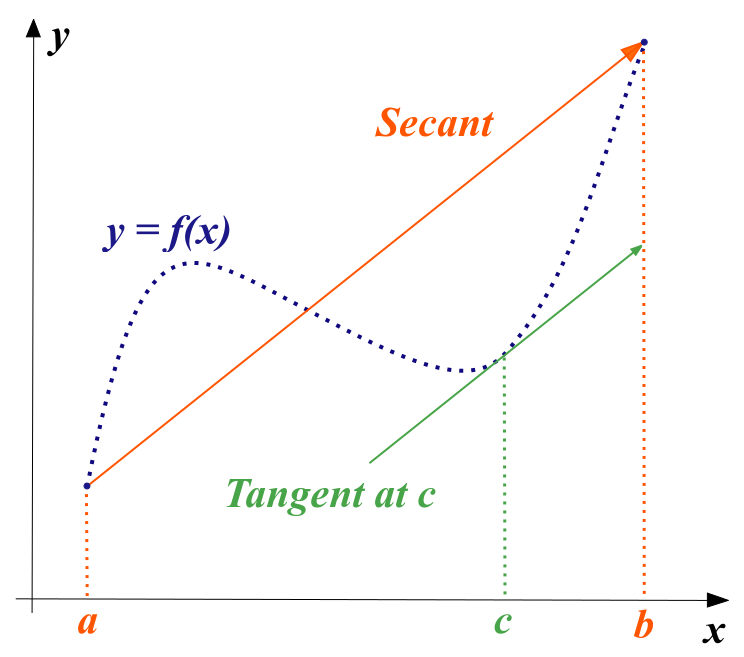
\includegraphics[width = 0.5\textwidth]{./applications_derivative/mvt.png}
	\caption{\hyperref{https://en.wikipedia.org/wiki/Mean\_value\_theorem}{}{}{Wikipedia - Mean Value Theorem}}
\end{figure}

\begin{example}
	A trucker drives 150 miles of a route in 2 hours.
	The speed limit along the route is 65 miles per hour.
	Show that at at least one point, the trucker must have been speeding.
\end{example}
\begin{answer}
	We can model the trucker's position along the route $s$ as a function of time $t$ where $s(0)=0$ and $s(2)=150$.
	We know that velocity is the derivative of position, so $v(t) = s^\prime(t)$.
	It's reasonable to assume that $s$ is differentiable on the interval $[0,2]$.
	So, by the Mean Value Theorem, there must exist a point $c$ where
	\begin{equation*}
		v(t) = \frac{s(2)-s(0)}{2-0} = \frac{150-0}{2} = 75\text{mph}.
	\end{equation*}
	At this point, the trucker was exceeding the speed limit of 65 miles per hour.
\end{answer}

\begin{definition}
	Let $f$ be defined on an interval $I$.
	Let $a$ and $b$ be any two different points in $I$.
	\begin{align*}
		\text{$f$ increases on $I$ if } a < b &\implies f(a) < f(b). \\
		\text{$f$ decreases on $I$ if } a < b &\implies f(a) > f(b).
	\end{align*}
\end{definition}

\begin{corollary}
	Let $f$ be continuous of $[a,b]$ and differentiable on $(a,b)$.
	\begin{align*}
		\text{If $f^\prime > 0$ at every point on $(a,b)$ then $f$ increases on $[a,b]$}. \\
		\text{If $f^\prime < 0$ at every point on $(a,b)$ then $f$ decreases on $[a,b]$}.
	\end{align*}
\end{corollary}

This should make sense given our theorem about local extrema.
If $f$ could still increase/decrease while its derivative was negative/positive, then we couldn't be sure that $f$ is at a local maxima/minima when $f^\prime=0$.

\begin{corollary}
	If $f^\prime(x) = 0$ at all points in an interval $I$, then there is some constant $C$ such that $f(x) = C$ for all points in $I$.
\end{corollary}

This follows from the Mean Value Theorem.
Since $f^\prime = 0$, the numerator in the Mean Value Theorem, $f(b) - f(a)$, must also be 0, meaning $f(b) = f(a) = C$.

\begin{corollary}
	If $f^\prime(x) = g^\prime(x)$ at every point in some interval $I$, then there is come constant $C$ such that $f(x) = g(x) + C$.
\end{corollary}

That is, functions with the same derivative differ by a constant.
This should make sense given our constant and sum and difference derivative rules.
If we let $h^\prime(x) = f^\prime(x) - g^\prime(x) = 0$ and apply the previous corollary, we get $C$.

\begin{definition}
	A function $F(x)$ is the antiderivative	of $f(x)$ if $F^\prime(x) = f(x)$ for all points in the domain of $f$.
\end{definition}

As we saw in the previous corollary, a function will have infinitely many antiderivatives that differ by a constant.
\section{First and Second Derivative Tests}
\subsection{First Derivative Test}
As we saw in previous sections, we can use the first derivative to find critical values, which allow us to find extrema.
\begin{theorem}[First Derivative Test]
	Let $f(x)$ be a continuous function.
	At a critical point $c$,
	\begin{enumerate}
		\item If $f^\prime$ changes sign from positive to negative ($f^\prime(x) > 0$ for $x < c$ and $f^\prime(x) < 0$ for $x > c$), then $f$ has a local maximum at $c$.
		\item If $f^\prime$ changes sign from negative to positive ($f^\prime(x) < 0$ for $x < c$ and $f^\prime(x) > 0$ for $x > c$), then $f$ has a local minimum at $c$.
		\item If $f^\prime$ does not change sign at $c$, then $f$ does not have a local extrema at $c$.
		\item At a left endpoint $a$, if ($f^\prime < 0$ / $f^\prime > 0$), then $f$ has a local (maximum / minimum) at $a$.
		\item At a right endpoint $b$, if ($f^\prime < 0$ / $f^\prime > 0$), then $f$ has a local (minimum / maximum) at $b$.
	\end{enumerate}
\end{theorem}

\begin{example}
	Find the local extrema of $f(x) = x^3 - 12x - 5$.
	Identify any absolute extrema.
\end{example}
\begin{answer}
	Taking the derivative,
	\begin{equation*}
		f^\prime(x) = 3x^2 - 12 = 3(x+2)(x-2).
	\end{equation*}
	
	So, the critical values are $x=-2$ and $x=2$.
	$f^\prime$ is negative between these values and positive outside of them, so $x=-2$ is a local maximum, while $x=2$ is a local minimum.
	\begin{equation*}
		f(-2) = 11 \text{ and } f(2) = -21.
	\end{equation*}
	
	As $x$ approaches $\infty$ (the right endpoint), $f$ also approaches $\infty$, so there is no absolute maximum.
	Similarly, as $x$ approaches $-\infty$ (the left endpoint), $f$ also approaches $-\infty$, so there is no absolute minimum.
\end{answer}

\subsection{Second Derivative Test}
The second derivative tells us how the derivative is changing.
Whether the derivative is increasing or decreasing describes the concavity.
\begin{definition}
	On some open interval $I$, the graph of a twice differentiable function $f(x)$ is
	\begin{enumerate}
		\item Concave up if $f^{\prime\prime} > 0$ on $I$.
		\item Concave down if $f^{\prime\prime} < 0$ on $I$.
	\end{enumerate}
\end{definition}


Concave up portions of a graph tend to look like valleys, while concave down portions tend to look like hills.
Unlike the first derivative, we can tell if a function is increasing or decreasing using concavity.
We can however say if the function is increasing or decreasing more or less rapidly.

\begin{figure}[H]
	\label{second_derivative_test}
	\centering
	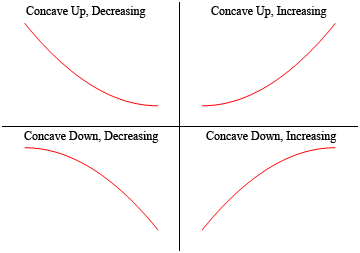
\includegraphics[width = 0.5\textwidth]{./applications_derivative/concavity.png}
	\caption{\hyperref{https://tutorial.math.lamar.edu/classes/calci/shapeofgraphptii.aspx}{}{}{Paul's Online Notes - The Shape of a Graph, Part II}}
\end{figure}


The points where a function changes concavity are called ``inflection points.''
At these points, the function is increasing or decreasing most rapidly, depending on the sign of the first derivative.


Rather than looking at the sign of $f^\prime$ around critical values, we can look at the concavity at the critical point.
\begin{theorem}[Second Derivative Test]
	Let $c$ be a critical value of $f$.
	\begin{enumerate}
		\item If $f^{\prime\prime}(c) < 0$, then $c$ is a local maximum.
		\item If $f^{\prime\prime}(c) > 0$, then $c$ is a local minimum.
		\item If $f^{\prime\prime}(c) = 0$, then the test is inclusive.
	\end{enumerate}
\end{theorem}

In other words, if we're at a critical point that's turning into a valley, then the critical point must be the top of a hill.
If we're at a critical point that's turning into a hill, then the critical point must be the bottom of a valley.
This test is particularly useful because you only need to know $f^{\prime\prime}$ at $c$ rather than an entire interval\footnote{It also extends to higher dimensions much better than the first derivative test.}.

\begin{example}
	Use the second derivative test to find the local extreme values of $f(x) = x^3 - 12x - 5$.
\end{example}
\begin{answer}
	Finding critical values,
	\begin{align*}
		f^\prime(x) &= 3x^2 - 12 = 3(x+2)(x-2). \\
		f^\prime(x) &= 0\text{ at } x=-2, x=2.
	\end{align*}
	
	Taking the second derivative,
	\begin{equation*}
		f^{\prime\prime}(x) = 6x.
	\end{equation*}
	
	Evaluating the second derivative at the critical values,
	\begin{equation*}
		f^{\prime\prime}(-2) = -12 \text{ and } f^{\prime\prime}(2) = 12.
	\end{equation*}
	
	So, $x=-2$ is a local maximum and $x=2$ is a local minimum.
\end{answer}
\section{Modeling \& Optimization}
Now that we know some ways to find extreme values, we can apply them to answer optimization problems.
The general steps needed to solve an optimization problem are:
\begin{enumerate}
	\item Write an equation that represents what you're trying to maximize/minimize. This is called your primary equation.
	\item Use additional information to eliminate excess variables.
	\item Find extreme values.
	\item Select the extreme values that fit the problem's constraints. Make sure your answer is what the problem is asking for.
\end{enumerate}

\begin{example}
	A farmer has 1000 linear feet of fence and wants to create a rectangular pasture.
	The pasture borders a river, which doesn't need a fence.
	What is the maximum area he can enclose?
\end{example}
\begin{enumerate}
	\item Since the pasture is rectangular, we know the two lengths of fence perpendicular to the river will be the same length, which we'll call $x$.
		We'll say the remaining side parallel to the river has length $y$.
		So, the area enclosed is
		\begin{equation*}
			A(x,y) = xy.
		\end{equation*}
	\item There is no reason for the farmer not to use all 1000 linear feet of fence, so we'd expect the sum of the lengths of the 3 fenced sides to be equal to 1000 feet: $2x + y = 1000$, or $y = 1000 - 2x$.
		We can then substitute back into our primary equation to get it in terms of just $x$.
		\begin{equation*}
			A(y) = x(1000-2x) = 1000x - 2x^2.
		\end{equation*}
	\item We'll do a first derivative test to find extreme values.
	\begin{align*}
		A^\prime(y) &= 1000 - 4x \\
		A^\prime(y) &= 0 \text{ at } x = 250 \\
		A^\prime(200) &= 200 > 0 \\
		A^\prime(300) &= -200 < 0.
	\end{align*}
	\item So, $x=250 \implies y = 500$ is a local maximum.
		This corresponds to an area of $A = 250\cdot 500 = 125000\text{ft}^2$.
\end{enumerate}

\begin{example}
	What is the maximum area of a rectangle that has two vertices on the $x-axis$ and two vertices on the portion of the graph $y=8-x^2$ where $y > 0$?
\end{example}
\begin{enumerate}
	\item We can define any such trapeziod (which include all such rectangles) by the $x$ values of the vertices on the $x$ axis.
		We'll call these two values $x_1$ and $x_2$.
		We'll say arbitrarily that $x_1 < x_2$.
		So, the area enclosed is
		\begin{equation*}
			A(x_1, x_2) = (x_2 - x_1)\frac{f(x_1) + f(x_2)}{2}.
		\end{equation*}
	\item However, the problem specifically restricts us to a rectangle, not a trapezoid.
		So, the heights of each side must be equal.
		\begin{align*}
			f(x_1) &= f(x_2) \\
			8 - x_1^2 &= 8 - x_2^2 \\
			x_1^2 &= x_2^2 \\
			\pm x_1 &\ \pm x_2 \\
			-x_1 &= x_2 \text{ because $x_1 \neq x_2$}.
		\end{align*}
		Substituting back into our primary equation,
		\begin{equation*}
			A(x_2) = (x_2 - (-x_2))\frac{f(x_2) + f(-x_2)}{2} = 2x_2f(x_2) = 16x_2 - 2x_2^3.
		\end{equation*}
	\item We'll do a second derivative test for fin extreme values.
		\begin{align*}
			A^\prime(x_2) &= 16 - 6x_2^2 \\
			A^\prime(x_2) &= 0 \text{ at } x = \pm\frac{4}{\sqrt{6}} \\
			A^{\prime\prime}(x_2) &= -12x_2 \\
			A^{\prime\prime}\left(-\frac{4}{\sqrt{6}}\right) &= 8\sqrt{6} > 0 \\
			A^{\prime\prime}\left(\frac{4}{\sqrt{6}}\right) &= -8\sqrt{6} < 0.
		\end{align*}
	\item So, $x_2 = 4/\sqrt{6}$ is a local maximum, and $x_2 = -4/\sqrt{6}$ is a local minimum.
		The problem asks for a maximum, so we select $x_2 = 4/\sqrt{6}$.
		The problem asks for a maximum area, so
		\begin{equation*}
			A_{max} = 16\left(\frac{4}{\sqrt{6}}\right) - 2\left(\frac{4}{\sqrt{6}}\right)^3 = \frac{128}{3\sqrt{6}} \approx 17.419.
		\end{equation*}
\end{enumerate}
\section{Related Rates}
In related rates problems, we generally have two related functions and want to know and answer questions about the rate of change of one function given that we know the rate of change of the other. The same problem solving steps as in modeling and optimization apply, but we'll usually be taking derivatives using implicit differentiation with respect to some variable like time.

\begin{example}
	Let $A$ be the area of a square with side length $x$.
	Assume that $x$ varies with time.
	How are $\dd{A}{t}$ and $\dd{x}{t}$ related?
	At a certain instant, the sides are 3 feet and growing at a rate of 2 feet per minute.
	How quickly is the area changing at this instant?
\end{example}
\begin{answer}
	Starting with the area of the square and implicitly differentiating with respect to $t$,
	\begin{align*}
		A &= x^2 \\
		\dd{A}{t} = 2x\dd{x}{t}.
	\end{align*}
	
	When $x=3\text{ft}$ and $\dd{x}{t}=3\text{ft/min}$,
	\begin{equation*}
		\dd{A}{t} = 2(3\text{ft})(3\text{ft/min}) = 12\text{ft$^2$/min}.
	\end{equation*}
\end{answer}

\begin{example}
	The top of a 13 foot ladder propped against a vertical wall begins falling towards the ground at 12ft/s.
	When the top of the ladder is 5 feet off the ground, how quickly is the bottom of the ladder moving away from the wall?
	How how is the angle between the ladder and the ground changing?
\end{example}
\begin{answer}
	Let $h$ be the height of the top of the ladder of the ground.
	Then $\dd{h}{t} = -12\text{ft/s}$.
	Let $b$ the the distance from the base of the ladder to the wall.
	We can relate $b$ and $h$ using the Pythagorean Theorem, where the 13-foot long ladder is the hypotenuse.
	\begin{equation*}
		b^2 + h^2 = 13^2.
	\end{equation*}
	
	We can also use this relationship to see that when $h=5\text{ft}$, $b=12\text{ft}$.
	Implicitly differentiating,
	\begin{equation*}
		2b\dd{b}{t} + 2h\dd{h}{t} = 0.
	\end{equation*}
	
	Plugging in what we know and solving for $\dd{b}{t}$,
	\begin{align*}
		2(12\text{ft})\dd{b}{t} + 2(5\text{ft})(-12\text{ft/s}) &= 0 \\
		24\text{ft}\dd{b}{t} &= 120\text{ft$^2$/s} \\
		\dd{b}{t} &= 5\text{ft/s}.
	\end{align*}
	
	So, the base of the ladder is moving away from the wall at a rate of 5ft/s.
	Let $\theta$ be the angle between the ladder and the ground.
	We can use $\sin$ to relate $\theta$ to $b$.
	\begin{equation*}
		13\sin{\theta} = b.
	\end{equation*}
	
	Implicitly differentiating,
	\begin{equation*}
		13\text{ft}\cos{(\theta)}\dd{\theta}{t} = \dd{b}{t}.
	\end{equation*}
	
	When $\cos$ is adjacent divided by hypotenuse, so $\cos{\theta} = 12/13$.
	Plugging in what we know and solving for $\dd{\theta}{t}$,
	\begin{align*}
		13\text{ft}(12/13)\dd{\theta}{t} &= -12\text{ft/s} \\
		\dd{\theta}{t} &= -1\text{/s}.
	\end{align*}
	
	So, the angle between the ladder and ground is decreasing at at rate of 1 rad/s.
\end{answer}

\begin{example}
	Grain is is poured at a rate of 10ft$^3$/min and falls into a cone-shaped pile whose bottom radius is half its altitude.
	How fast will the circumference of the base be increasing when the pile is 8 ft tall?
\end{example}
\begin{answer}
	Let $h$ the the altitude of the cone.
	At the instant we care about $h=8\text{ft}$.
	Let $r$ be the bottom radius of the cone.
	At the instant we care about, $r=h/2=4\text{ft}$.
	Let $V$ be the volume of the cone.
	We know that $\dd{V}{t}=10\text{ft$^3$/s}$.
	We can relate these three quantites using the formula for the volume of a cone.
	\begin{equation*}
		V = \frac{1}{3}\pi r^2 h.
	\end{equation*}
	
	Since we know that $2r = h$, we can simplify to get rid of $h$.
	\begin{equation*}
		V = \frac{2}{3}\pi r^3
	\end{equation*} 
	
	Implicitly differentiating,
	\begin{equation*}
		\dd{V}{t} = 2\pi r^2 \dd{r}{t}.
	\end{equation*}
	
	We know the formula for the circumference $C$ of the circular base.
	\begin{equation*}
		C = 2\pi r.
	\end{equation*}
	
	Implicitly differentiating,
	\begin{equation*}
		\dd{C}{t} = 2\pi \dd{r}{t}.
	\end{equation*}
	
	We can substitute into our equation involving $\dd{V}{t}$.
	\begin{equation*}
		\dd{V}{t} = r^2\dd{C}{t}.
	\end{equation*}
	
	Plugging in what we know,
	\begin{align*}
		10\text{ft}^3\text{/s} &= (4\text{ft})^2\dd{C}{t} \\
		\dd{C}{t} &= \frac{5}{8}\text{ft/s}.
	\end{align*}
\end{answer}

\section{Linearization \& Newton's Method}

\subsection{Linearization}
As we've seen, tangent lines intersect their function at most once: at the point of tangency.
However, we know that differentiable functions are locally linear, so we'd expect the tangent line to be a decent approximation of the function near the point of tangency.

\begin{definition}
	If $f$ is differentiable at $a$, then the approximating function
	\begin{equation*}
		L(x) = f^\prime(a)(x-a) + f(a)
	\end{equation*}
	is the linearization of $f$ at $a$.
\end{definition}

\begin{example}
	Find the linearization of $f(x) = \ln{(x+1)}$ at $x=0$.
	How accurate is this approximation at $x=0.1$?
\end{example}
\begin{answer}
	Following the definition,
	\begin{align*}
		f(0) = \ln{(0+1)} = 0 \\
		f^\prime(x) &= \frac{1}{x+1} \\
		f^\prime(0) &= \frac{1}{0+1} = 1 \\
		L(x) &= 1(x-0) + 0 = x.
	\end{align*}
	
	Calculating the error at $x=0.1$,
	\begin{align*} 
		L(0.1) &= 0.1 \\
		f(0.1) &\approx .0953 \\
		\text{\% error} &= \frac{\abs{L(0.1)-f(0.1)}}{L(0.1)}100\text{\%} \approx 4.7\text{\%}.
	\end{align*}
	
	So, we can see the linear approximation is pretty good.
\end{answer}


We call the difference in $x$ between the point of tangency and the point we're trying to approximate the differential.
\begin{definition}
	Let $y=f(x)$ be a differentiable function.
	The differential $\d{x}$ is an independent variable.
	The differential $\d{y}$ is $\d{y} = f^\prime(x)\d{x}$.
\end{definition}

$\mathrm{d}y$ is the approximated change in $y$ expected by the linearization for some given change in $x$, $\d{x}$.

\begin{example}
	Find $\d{y}$ for $y=\frac{2x}{1+x^2}$, $x=-2$, and $\d{x} = 0.1$.
\end{example}
\begin{answer}
	\begin{align*}
		y^\prime &= \frac{-4x^2}{\left(1+x^2\right)^2} + \frac{2}{1+x^2} \\
		y^\prime(-2) &= -6/25 \\
		\d{y} &= (-6/25)(0.1) = -0.024.
	\end{align*}
\end{answer}

\subsection{Newton's Method}
We can use the fact that the tangent line approximates the function to find the zeroes of functions.
Starting with an initial guess $x_0$ for the $x$ value of the zero, we look at the the tangent line at $x_0$ and find where it intersects the $x-axis$.
\begin{align*}
	L_0(x) &= f^\prime(x_0)(x - x_0) + f(x_0) \\
	0 &= f^\prime(x_0)(x - x_0) + f(x_0) \\
	-f^\prime(x_0)(x - x_0) &= f(x_0) \\
	x - x_0 &= -\frac{f(x_0)}{f^\prime(x_0)} \\
	x &= x_0 - \frac{f(x_0)}{f^\prime(x_0)}.
\end{align*}
This $x$ value serves as our next guess for the zero.
We repeat this process, until we find the zero or are satisfied with our error\footnote{For most well-behaved functions, Newton's Method can get within a small margin of error or a zero relatively quickly. There is also a generalized, sometimes faster version of Newton's Method that approximates the function with higher-order polynomials than just lines.}.
This yields a recursive formula
\begin{equation*}
	x_{n+1} = x_n - \frac{f(x_n)}{f^\prime(x_n)}.
\end{equation*}
		\subsubsection{Integrals}
The definite integral of a function $f(x)$ from $x=a$ to $x=b$ where $a \leq b$ is the area between $f(x)$ and the $x$-axis bounded by the lines $x=a$ and $x=b$ where area above the $x$-axis is positive, and area below the $x$-axis is negative. 
\begin{definition}
	\begin{equation*}
		\int_{a}^{b}{f(x) \mathrm{d}x} = \lim\limits_{h \to 0}{\sum_{n=1}^{\frac{b-a}{h}}}{f(a + (n-1)h) \cdot h}.
	\end{equation*}
\end{definition}

\noindent
We also define an indefinite integral, or antiderivative of $f(x)$, notated $F(x)$ where
\begin{equation*}
F'(x) = f(x) \implies \int{f(x)\mathrm{d}x} = F(x).
\end{equation*}
Note that there are infinitely many such functions $F$, since adding a constant to $F$ does not affect its derivative. To notate this, we add a constant $C$ to the indefinite integral. Given an initial condition for $f$, we can solve for $C$.\\

\noindent
Below are some properties of the integral. Let $f$ and $g$ be functions of $x$ and $p$, $a$, $b$, and $c$ where $a < b < c$, and $f$ and $g$ are continuous on the closed interval $[a,c]$.
\begin{enumerate}[label=]
	\item \textbf{Linearity}
	\begin{equation*}
		\int{(pf \pm g) \mathrm{d}x} = p\int{f \mathrm{d}x} \pm \int{g \mathrm{d}x}
	\end{equation*}
	\item \textbf{Flipped Bounds}
	\begin{equation*}
		\int_{a}^{b}{f \mathrm{d}x} = -\int_{b}^{a}{f \mathrm{d}x}
	\end{equation*}
	\item \textbf{Union of Intervals}
	\begin{equation*}
		\int_{a}^{b}{f \mathrm{d}x} + \int_{b}^{c}{f \mathrm{d}x} = \int_{a}^{c}{f \mathrm{d}x}
	\end{equation*}
	\item \textbf{Power Rule}
	\begin{equation*}
		\int{x^n \mathrm{d}x} = \frac{x^{n+1}}{n+1} + C \text{, }n \neq -1
	\end{equation*}
	\item \textbf{U-Substitution}
	\begin{equation*}
		\int{\left(f'\circ g\right) g' \mathrm{d}x} = f\circ g+ C
	\end{equation*}
	\item \textbf{Integration by Parts}
	\begin{equation*}
		\int{f' g \mathrm{d}x} = fg - \int{fg' \mathrm{d}x}
	\end{equation*}
	\item \textbf{Fundamental Theorem of Calculus}
	\begin{equation*}
		\dd{}{x}\int_{a}^{x}{f(s) \mathrm{d}s} = f(x)
	\end{equation*}
\end{enumerate}
Using the definition of the integral and the above rules, we can find the indefinite integral of some common functions.
\begin{align*}
	\int{\frac{1}{x} \mathrm{d}x} &= \ln{\abs{x}} + C \\
	\int{\sin{x} \mathrm{d}x} &= -\cos{x} + C \\
	\int{\cos{x} \mathrm{d}x} &= \sin{x} + C \\
	\int{\tan{x} \mathrm{d}x} &= -\ln{\abs{\cos{x}}} + C
\end{align*}
		\chapter{Applications of Integrals}

\section{Physics}
\subsection{Position, Velocity, \& Acceleration}
Since we know by the FTC that integration is the opposite of differentiation, we can also interpret integrals in a similar physical sense as derivatives.
\begin{table}[H]
	\begin{center}
		\begin{tabular}{ l l }
			$\begin{aligned}\int{v(t)\d{t}}=x(t) + C\end{aligned}$ & $\begin{aligned}\int{a(t)\d{t}}=v(t)\end{aligned}$
		\end{tabular}
	\end{center}
\end{table}

\begin{example}
	A particle starts at $t=0$ with an initial velocity of 5m/s and accelerates for 8 seconds.
	Its acceleration is given by $a(t)=2.4t$ m/s$^2$.
	What is the particle's velocity after the 8 seconds pass?
	What is the particle's displacement after the 8 seconds pass?
\end{example}
\begin{answer}
	We can integrate acceleration to get velocity.
	\begin{equation*}
		v(t) = \int{2.4t\d{t}} = 1.2t^2 + C.
	\end{equation*}
	
	We know that $v(0)=5$m/s so we can solve\footnote{When we solve for $C$ like this, we're solving what's called an "inital value problem," which we'll do more of when talking about differential equations.} for $C$.
	\begin{align*}
		1.2(0) + C &= 5 \\
		C &= 5 \\
		v(t) = 1.2t^2 + 5.
	\end{align*}
	
	So, at $t=8$, $v(8) = 1.2(8)^2 + 5 = 81.8$m/s.
	We can now integrate velocity to get displacement
	\begin{equation*}
		x(t) = \int{1.2t^2 + 5 \d{t}} = 0.4t^3 + 5t + C.
	\end{equation*}
	
	We know that $x(0)=0$m, so $C=0$.
	\begin{equation*}
		x(t) = 0.4t^3 + 5t.
	\end{equation*}
	
	So, at $t=8$, $x(t) = 0.4(8)^3 + 5(8) = 244.8$m.
	We could have also tackled this problem with definite integrals.
	\begin{align*}
		\Delta x = \int_{0}^{8}{v(t)\d{t}} &= 244.8\text{m} \implies \text{Net Displacement} = x_0 + \Delta x = 244.8\text{m} \\
		\Delta v = \int_{0}^{8}{a(t)\d{t}} &= 76.8\text{m/s} \implies \text{Net Velocity} = v_0 + \Delta v = 81.8\text{m/s}
	\end{align*}
\end{answer}

\subsection{Work}
Work is defined as
\begin{equation*}
	W = Fd
\end{equation*}
where $F$ is force and $d$ is displacement.
The force applied by stretching or compressing a spring beyond its natural length is given by Hooke's Law
\begin{equation*}
	F = kx
\end{equation*}
where $k$ is some spring constant and $x$ is the displacement beyond the spring's natural length.
We can apply ideas as integrals representing net change to find the work needed to compress or stretch a spring.

\begin{example}
	It takes 10N of force to stretch a spring 2m beyond its natural length.
	How much work is done stretching the spring 4m beyond its natural length?
\end{example}
\begin{answer}
	We can use the first bit of information to get the spring constant.
	\begin{align*}
		F &= kx \\
		10\text{N} &= k(2\text{m}) \\
		k &= 5\text{N/m}.
	\end{align*}
	
	So, $F(x)=5x\text{N}$.
	If we stretch the spring by $\Delta x$, the work done over this interval is approximately $\Delta W = F(x)\Delta x= 5x\Delta x$.
	In the limit, $\d{W} = 5x\d{x}$.
	Integrating both sides from $x=0$ to $x=4$,
	\begin{equation*}
		W = \int_{0}^{4}{\d{W}} = \int_{0}^{4}{5x\d{x}} = 40\text{Nm}.
	\end{equation*}
\end{answer}


We can even bring in other concepts to these problems, like related rates.
\begin{example}
	An inverted conical tank with a height of 10ft and a base radius of 5ft is filled to within 2ft of the top with a liquid with a density of 57lbs/ft$^3$.
	How much work does it take to fill the remaining 2ft of the tank with liquid, assuming you only have to pump the liquid to the current liquid level in the tank?
\end{example}
\begin{answer}
	Let $V$ be the volume of the tank and $x$ the height of the liquid.
	Imagine we pump in some liquid that changes the height of the liquid in the tank by $\Delta x$.
	Then
	\begin{align*}
		\Delta V &= \pi r^2 \Delta x \\
		\d{V} &= \pi r^2 \d{x}.
	\end{align*}
	
	Since the height of the tank is 10ft and the base radius 5ft, the radius of the liquid level will always be half the liquid depth.
	\begin{align*}
		r &= x/2 \\
		\d{V} &= \pi (x/2)^2 \d{x}.
	\end{align*}
	
	Since weight in pounds is already a unit of force, we can multiply $\d{V}$ by the density of the liquid to get $F$.
	\begin{equation*}
		F = 57\pi(x/2)^2 \d{x}.
	\end{equation*}
	
	The displacement of the liquid is the current height of the liquid $x$, getting us $\d{W}$.
	\begin{align*}
		\d{W} &= 57\pi x(x/2)^2 \d{x} \\
		W &= \int_{8}^{10}{57\pi x(x/2)^2 \d{x}} \\
		&= 21033\pi \text{ft lbs}.
	\end{align*}
\end{answer}


\section{Lengths of Curves}
If we're at some point $(x,f(x))$ and move $\d{x}$ units over, we'll be at a new point $(x+\d{x},f(x+\d{x}))$.
This point is $\d{x}$ units horizontally and $\d{y}=f(x+\d{x})-f(x)$ vertically away from $(x,f(x))$.
So, by the Pythagorean Theorem, the new point is $\d{s} = \sqrt{(\d{x})^2+(\d{y})^2}$ units away.

\begin{figure}[H]
	\label{arclength}
	\centering
	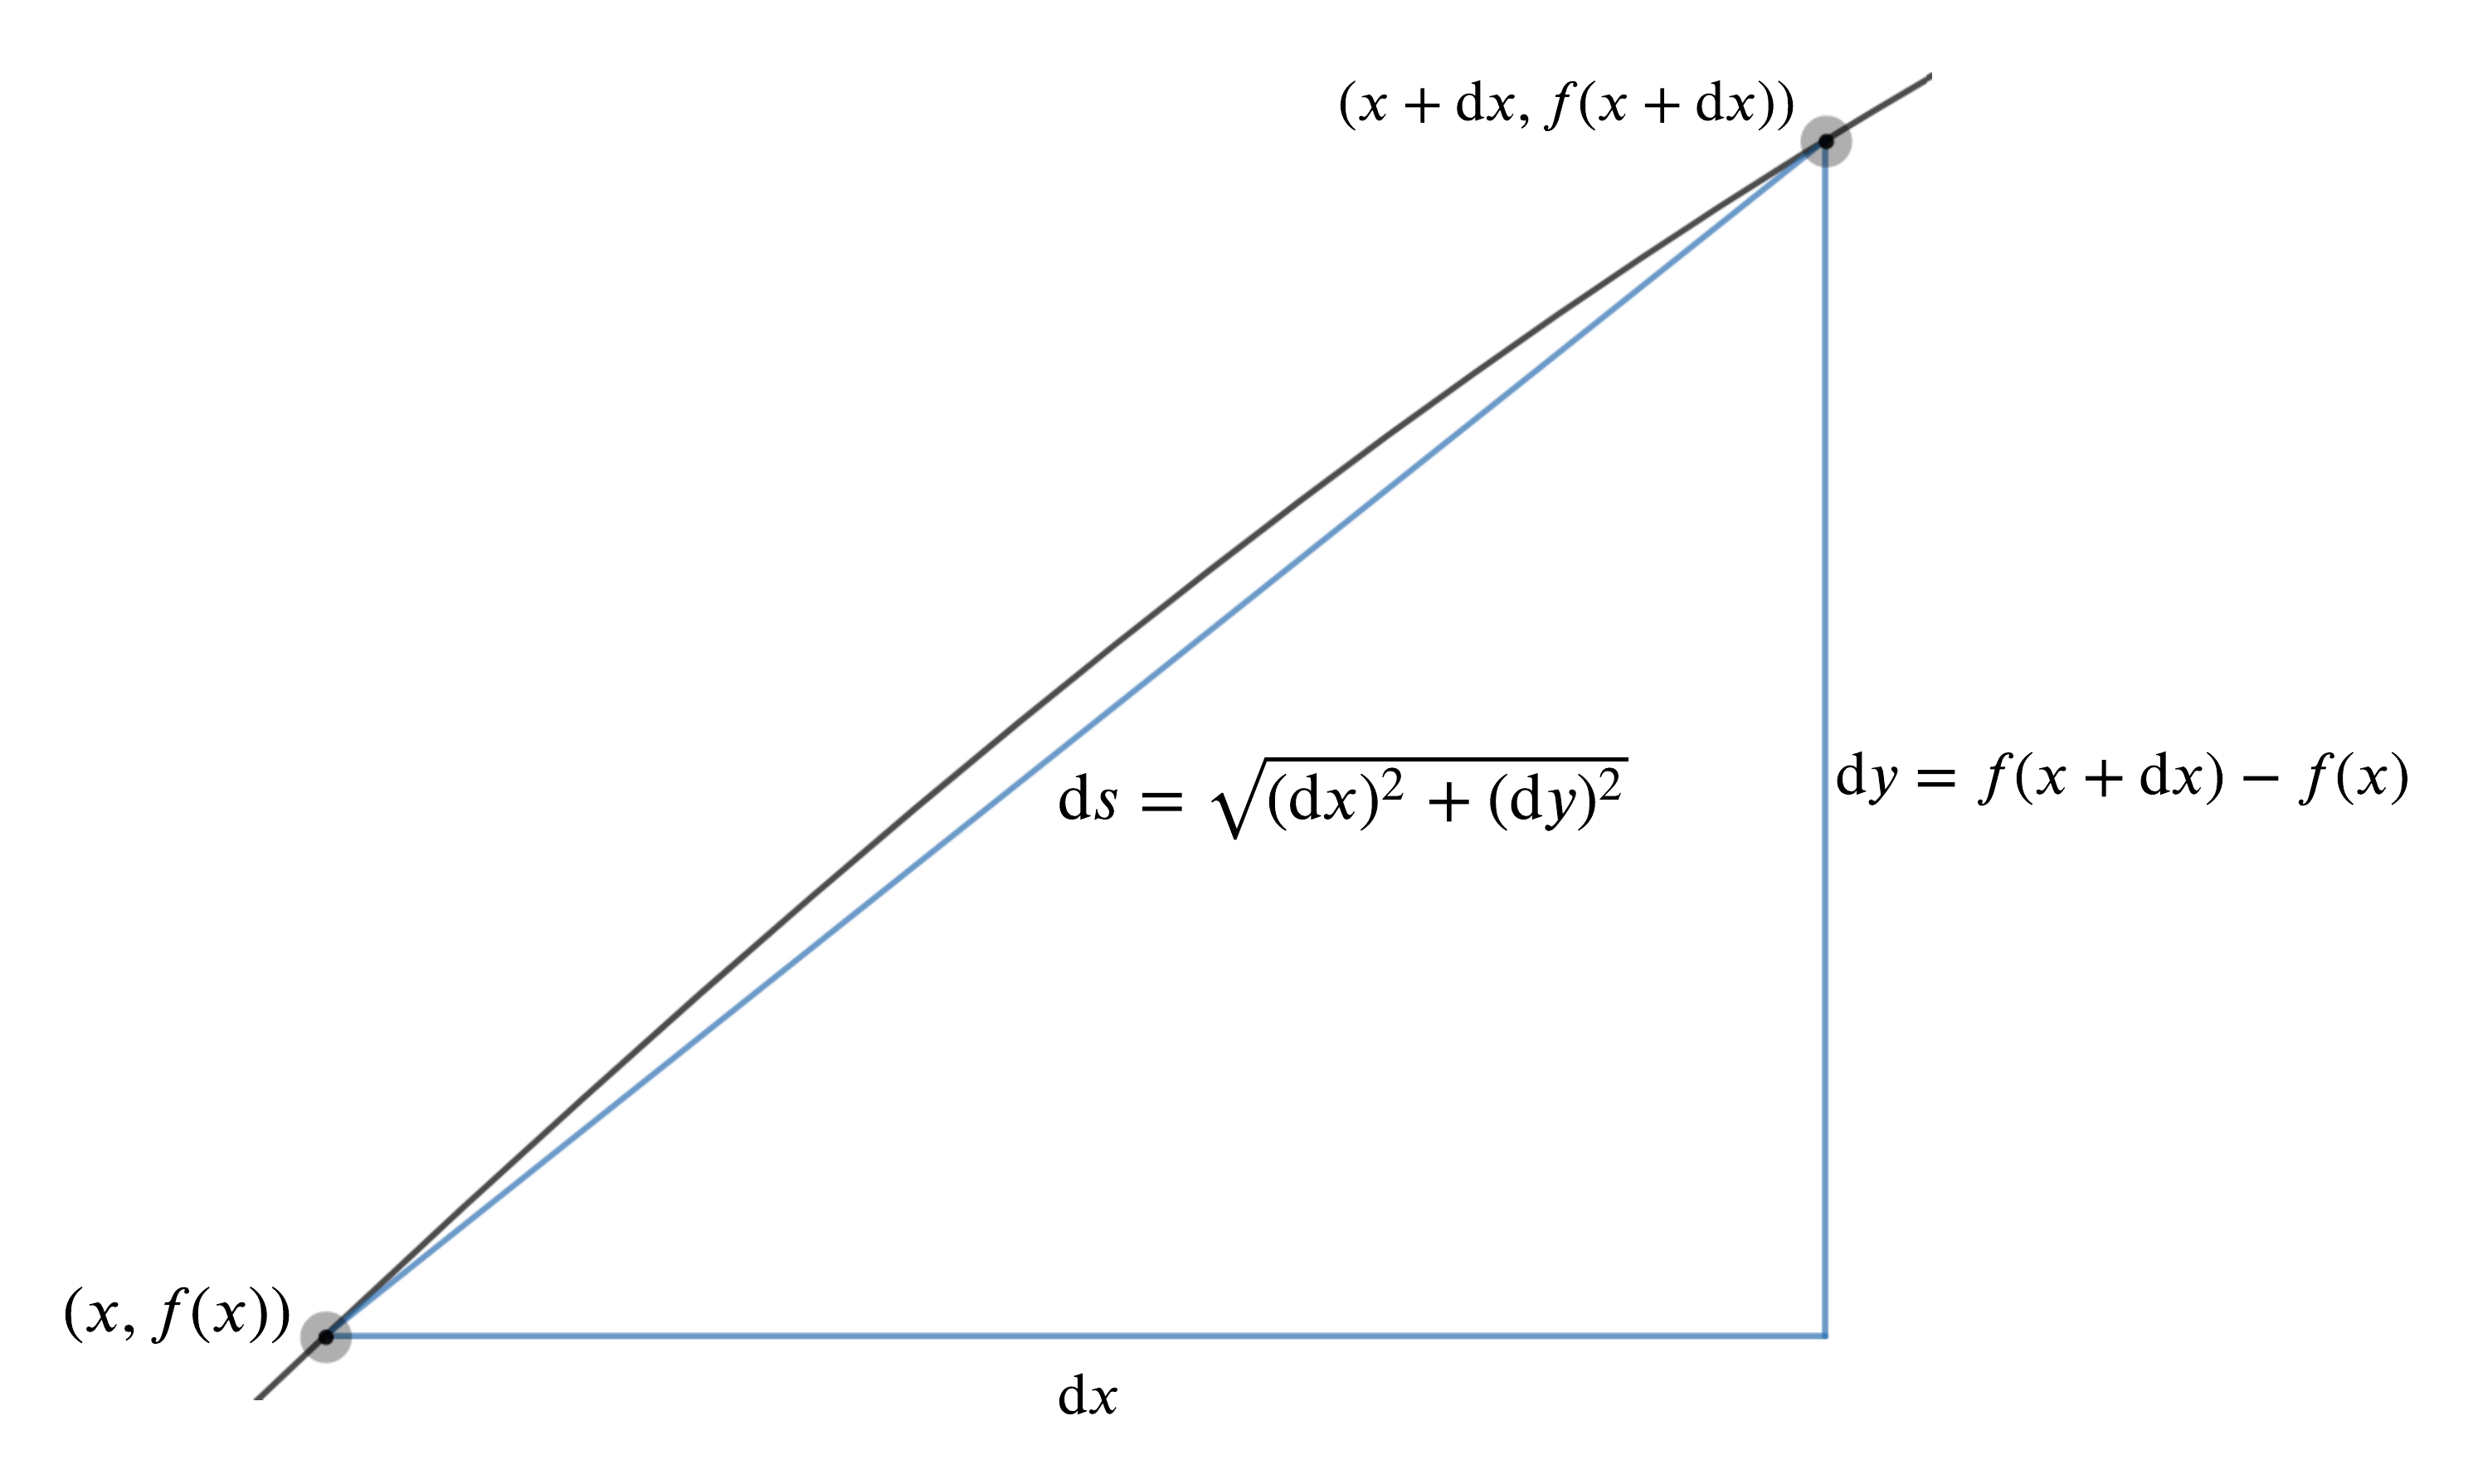
\includegraphics[width=0.66\textwidth]{./applications_integrals/arclength.png}
	\caption{\hyperref{}{}{}{Secant length approaches arc length}}
\end{figure}
\noindent
As $\d{x}$ approaches 0, $\d{s}$, the length of the secant line, approaches the length of the curve.
If we summed all of these $\d{s}$'s in some interval we'd have the length of the curve on that interval.
\begin{align*}
	s &= \int_{a}^{b}{\d{s}} \\
	&= \int_{a}^{b}{\sqrt{(\d{x})^2+(\d{y})^2}} \\
	&= \int_{a}^{b}{\sqrt{(\d{x})^2\left(1+\left(\frac{\d{y}}{\d{x}}\right)^2\right)}} \\
	&= \int_{a}^{b}{\sqrt{1+\left(\frac{\d{y}}{\d{x}}\right)^2}\d{x}}.
\end{align*}

\begin{example}
	Show that the circumference of a circle with radius $r$ is $C=2\pi r$.
\end{example}
Starting with the equation of a circle of radius $r$ and implicitly differentiating,
\begin{align*}
	x^2 + y^2 &= r^2 \\
	2x + 2y\dd{y}{x} &= 0 \\
	\dd{y}{x} &= \frac{-x}{y} \\
	\left(\dd{y}{x}\right)^2 &= \frac{x^2}{y^2} = \frac{x^2}{r^2-x^2} \\
	C &= 2\int_{-r}^{r}{\sqrt{1+\frac{x^2}{r^2-x^2}}\d{x}} \\ 
	&\text{ (2 b/c we need to count upper and lower half)} \\
	&= 2\int_{-r}^{r}{\sqrt{\frac{r^2}{r^2-x^2}}\d{x}} \\
	&= 2\int_{-r}^{r}{r\sqrt{\frac{1}{r^2-x^2}}\d{x}} \\
	&= 2r\arcsin{\left(\frac{x}{r}\right)}\biggr\rvert_{-r}^{r} \\
	&= 2\pi r.
\end{align*}

\noindent
Note that when deriving the arc length formula, we could have just as easily have divided by $(\d{y})^2$.
This would give us an equivalent arc length formula that's applicable when $x$ is a function of $y$.

\begin{example}
	Find the length of the curve $y=x^{1/3}$ from $(-8,2)$ to $(8,2)$.
\end{example}
Rather than  tediously integrate the square root of a cube root if we set our bounds in terms of $x$, we can rewrite our equation and set out bounds in terms of $y$.
\begin{align*}
	x &= y^3 \\
	\dd{x}{y} &= 3y^2 \\
	\left(\dd{x}{y}\right)^2 &= 9y^4 \\
	s &= \int_{-2}^{2}{\sqrt{1+9y^4}\d{y}} \\
	&\footnotemark\approx 17.261.
\end{align*}
\footnotetext{You shouldn't be expected to evaluate this integral analytically. Using a calculator is fine.}
\section{Areas in the Plane}
\begin{lemma}
	If $f(x) \geq g(x)$ on $[a,b]$ then the area between $f(x)$ and $g(x)$ on $[a,b]$ is given by
	\begin{equation*}
		A = \int_{a}^{b}{\left(f(x)-g(x)\right)\d{x}}.
	\end{equation*}
\end{lemma}
\noindent
You can easily visualize why this is true.
We can break the integral into two parts: adding the area under $f$ and the other subtracting the area under $g$.
The first integral will over count the area between $f$ and $g$, counting all area between $f$ and the $x$-axis.
The second integral will subtract exactly the amount of area that is over counted: the area that is also between $g$ and the $x$-axis.

\begin{figure}[H]
	\label{area_between_curves}
	\centering
	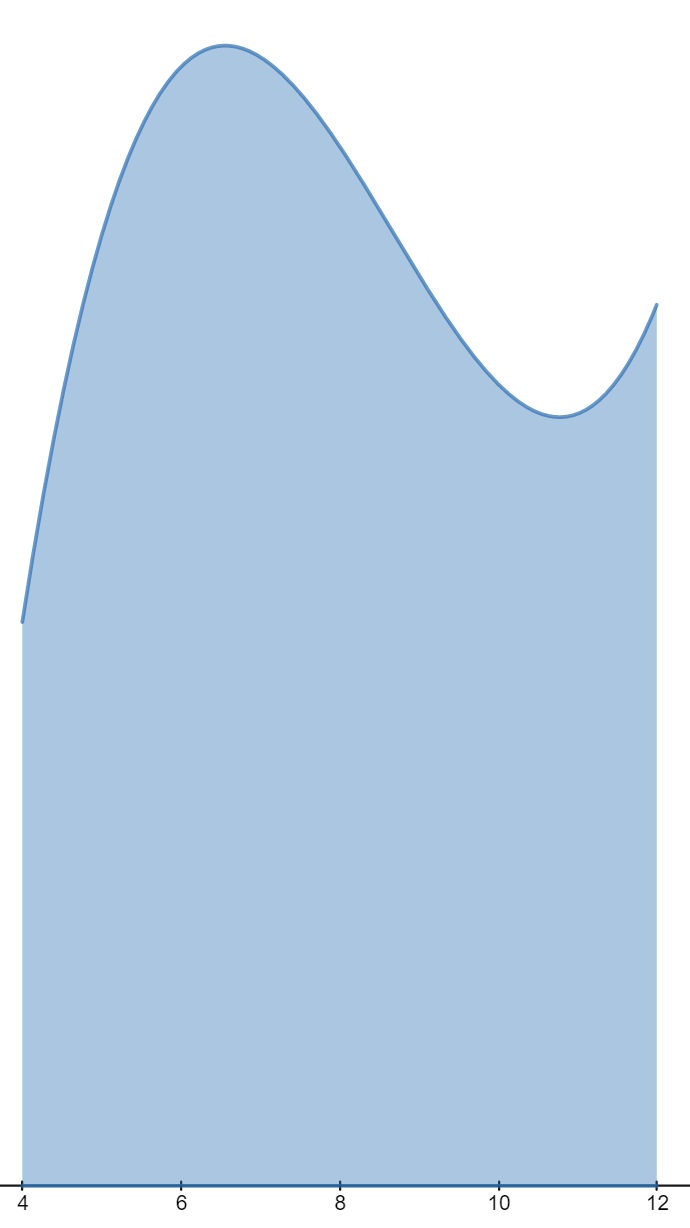
\includegraphics[width = 0.33\textwidth]{./applications_integrals/curve1.png}
	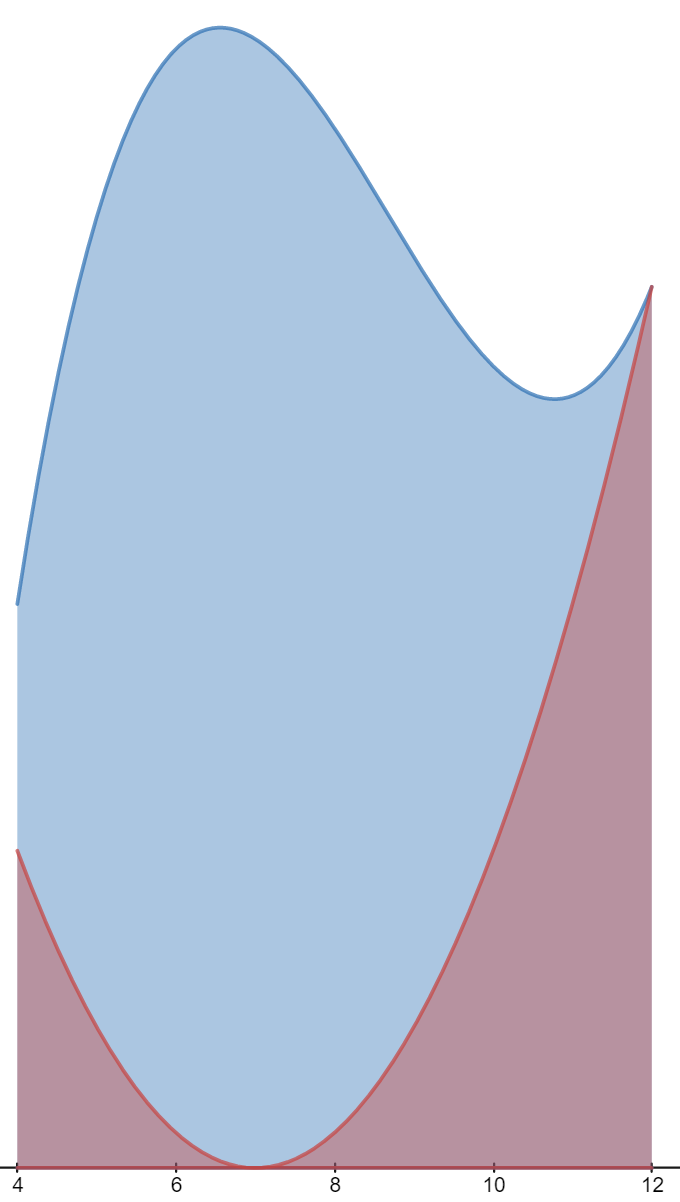
\includegraphics[width = 0.33\textwidth]{./applications_integrals/curve2.png}
	\caption{\hyperref{}{}{}{Subtracting two areas to get the area between them}}
\end{figure}
\noindent
Even if both of the curves has more area below the $x$-axis, the same idea applies.
$f$ will give a smaller-magnitude negative area, while $g$ will give a larger magnitude negative area.
Subtracting a larger-magnitude negative number from a smaller magnitude negative number will give a positive area.

\begin{example}
	Find the area enclosed between the two curves $y=2-x^2$ and $y=-x$.
\end{example}
These two curves intersect at $x=-1$ and $x=2$.
Applying the formula,
\begin{align*}
	A &= \int_{-1}^{2}{((2-x^2)-(-x))\d{x}} \\
	&= 2x-\frac{x^3}{3} + \frac{x^2}{2}\biggr\rvert_{-1}^{2} \\
	&= \frac{9}{2}.
\end{align*}

\subsection{Subregions}
Sometimes it might be useful to break the enclosed regions into subregions and find the area of each separately.
\begin{example}
	Find the area above the $x$-axis, below $y=\sqrt{x}$, and above $y=x-2$.
\end{example}
If we simply took the area between the two curves, we'd count some area we don't want beneath the $x$-axis\footnote{Although this extra region is just a triangle and not too hard to find the area of, you'd effectively be applying the same strategy of two subregions, they'd just overlap. However, using geometry to your advantage is certainly a valid approach.}.
Instead, we can break the area into two subregions: one between the $x$-axis and $\sqrt{x}$ and the other between $x-2$ and $\sqrt{x}$.
\begin{figure}[H]
	\label{subregions}
	\centering
	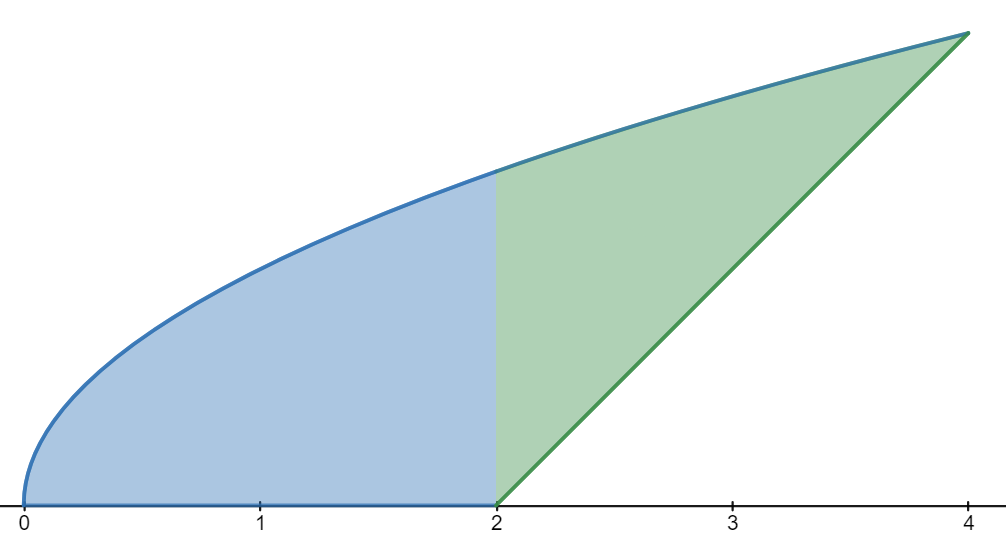
\includegraphics[width = 0.33\textwidth]{./applications_integrals/two_regions.png}
	\caption{\hyperref{}{}{}{Break complicated areas into simpler subregions}}
\end{figure}
\indent
Finding the area of the blue region,
\begin{equation*}
	A_1 = \int_{0}^{2}{\sqrt{x}\d{x}} = \frac{2x\sqrt{x}}{3}\biggr\rvert_0^2 = \frac{4\sqrt{2}}{3}.
\end{equation*}
\indent
Finding the area of the green region,
\begin{equation*}
	A_2 = \int_{2}^{4}{(\sqrt{x}-(x-2))\d{x}} = \frac{2x\sqrt{x}}{3} - \frac{x^2}{2} + 2x \biggr\rvert_2^4 = \frac{10}{3} - \frac{4\sqrt{2}}{3}.
\end{equation*}
\indent
Adding the areas of the two regions,
\begin{equation*}
	A = A_1 + A_2 = \frac{10}{3}.
\end{equation*}

\subsection{Integrating by $y$}
Another strategy when finding the area of more complex regions is to see if they become easier to deal with if we were to instead integrate with respect to $y$.
In the above example, it is indeed easier to work with respect to $y$ because both bounding curves are between the same $y$ values.
\begin{example}
	Find the area above the $x$-axis, below $y=\sqrt{x}$, and above $y=x-2$.
\end{example}
We need to rearrange our equations to be of the form $x=\ldots$ instead of $y=\ldots$ by simply solving for $x$.
\begin{equation*}
	x = y^2, y\geq 0 \text{ and } x = y+2.
\end{equation*}
\indent
Since $x=y+2$ is further from the $x$-axis, it becomes our top curve.
\begin{align*}
	A &= \int_{0}^{2}{((y+2)-y^2)\d{y}} \\
	&= \frac{y^2}{2} + 2y - \frac{y^3}{3} \biggr\rvert_0^2 \\
	&= \frac{10}{3}.
\end{align*}
\section{Volumes}
\subsection{Volumes from Cross Sections}
Imagine we want to find the volume of some complex object.
One way we could approximate it is by slicing it into narrow cross sections.
The volume of each cross section would roughly be the area of the cross sectional face, times the width of the cross section.

\begin{figure}[H]
	\label{volumes}
	\centering
	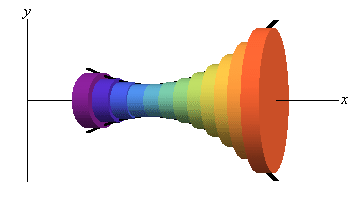
\includegraphics[width=0.5\textwidth]{./applications_integrals/volumes.png}
	\caption{\hyperref{https://tutorial.math.lamar.edu/classes/calci/Area\_Volume\_Formulas.aspx}{}{}{Paul's Online Notes - Area and Volume Formulas}}
\end{figure}

Adding the volumes of these cross sections up, we'd get our approximation, which would get better and better the narrower the width of each cross section.
In the limit, this is exactly the definition of an integral.

\begin{definition}
	The volume of a solid with integrable corss sectional area $A(x)$ from $x=a$ to $x=b$ is given by
	\begin{equation*}
		V = \int_{a}^{b}{A(x)\d{x}}.
	\end{equation*}
\end{definition}


Let's start by finding the volume of a solid we already know.
\begin{example}
	Find the volume of a cube with sidelength $a$.
\end{example}
\begin{answer}
	For any slice of a cube, the cross section is a square with sidelength $a$.
	\begin{align*}
		A(x) &= a^2 \\
		V &= \int_{0}^{a}{a^2\d{x}} \\
		&= a^2x\biggr\rvert_0^a \\
		&= a^3.
	\end{align*}
\end{answer}


Now let's find the volume of a slightly more complicated shape.
\begin{example}
	Find the volume of a square pyramid with base sidelength $a$ and height $h$.
\end{example}
\begin{answer}
	Like the cube, any slice of the square pyramid is a square.
	However, the sidelength of the square depends on the height of your slice.
	A slice at the very tip of the pyramid would have sidelength 0, while a slice at the very bottom of the pyramid would have sidelength $a$.
	The sidelength grows linearly from $x=0$ to $x=h$, so it must be $\frac{a}{h}x$.
	\begin{align*}
		A(x) &= \left(\frac{a}{h}x\right)^2 \\
		V &= \int_{0}^{h}{\frac{a^2}{h^2}x^2\d{x}} \\
		&= \frac{a^2}{3h^2}x^3 \biggr\rvert_0^h \\
		&= \frac{a^2h}{3} \\
		&= \frac{1}{3}a^2 h.
	\end{align*}
\end{answer}

\subsection{Solids of Revolution}
You can think of solids of revolution as a special case of volumes from cross sections.
We'll tend to be on the lookout for a function that defines the radius, and we can then use the formula for the area of a circle to get the cross sectional area.
\begin{equation*}
	A(x) = \pi r^2(x).
\end{equation*}

\begin{example}
	Find the volume of the cone formed by rotating the line $y=x/3$ about the $x$-axis for $0 \leq x \leq 6$.
\end{example}
\begin{answer}
	The radius is simply the distance from the $x$-axis, which is just another name for $y$.
	So,
	\begin{equation*}
		A(x) = \pi \left(\frac{x}{3}\right)^2.
	\end{equation*}
	
	Integrating,
	\begin{align*}
		V &= \int_{0}^{6}{\pi\left(\frac{x}{3}\right)^2\d{x}} \\
		&= \frac{\pi}{9}\int_{0}^{6}{x^2\d{x}} \\
		&= \frac{\pi}{9}\left(\frac{x^3}{3}\biggr\rvert_0^6\right) \\
		&= 8\pi.
	\end{align*}
	
	This is the volume of a cone with radius 2 and height 6: $\frac{1}{3}\pi(2)^2(6)=8\pi$.
\end{answer}


Let's try a more complicated solid.
\begin{example}
	Find the volume of the solid of revolution bounded by $y=2+x\cos{x}$ from $-\frac{\pi}{2} \leq x \leq \frac{\pi}{2}$.
\end{example}
\begin{answer}
	Again, the radius is simply the distance from the $x$-axis, which is $y$.
	\begin{align*}
		A(x) &= \pi \left(2+x\cos{x}\right)^2 \\
		&= \pi \left(4 + 4x\cos{x} + x^2\cos^2{x}\right) \\
		V &= \int_{-\pi/2}^{\pi/2}{\pi \left(4 + 4x\cos{x} + x^2\cos^2{x}\right)\d{x}} \\
		&= \pi\left(\int_{-\pi/2}^{\pi/2}{4\d{x}}+\int_{-\pi/2}^{\pi/2}{4x\cos{x}\d{x}}+\int_{-\pi/2}^{\pi/2}{x^2\cos^2{x}\d{x}}\right) \\
		&= \pi\left(4\pi + 0 + \frac{1}{24}\pi\left(\pi^2-6\right)\right) \text{ (use integration by parts)}\\
		&= \frac{\pi^4}{24} + \frac{15\pi^2}{4}.
	\end{align*}
\end{answer}

\subsubsection{Washer Method}
Imagine now we want to find the volume of a solid of revolution with a ``hole.``
''If we were to take a cross section of such a solid, it'd look like a washer with an outer radius $R(x)$ and inner radius $r(x)$.

\begin{figure}[H]
	\label{washers}
	\centering
	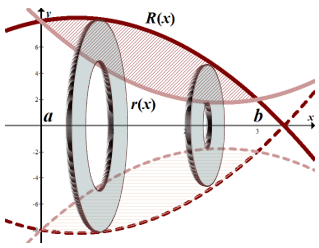
\includegraphics[width=0.33\textwidth]{./applications_integrals/Washer-1.png}
	\caption{\hyperref{https://www.shelovesmath.com/calculus/integral-calculus/applications-integration-area-volume/}{}{}{She Loves Math - Applications of Integration: Area and Volume}}
\end{figure}


We can think of this in a similar way as the area between curves in 2D.
We'll find the volume swept by the outer radius and the subtract the volume swept and removed by the inner radius.
\begin{equation*}
	V = \pi\int_{a}^{b}{(R^2(x)-r^2(x))\d{x}}.
\end{equation*}

\begin{example}
	Find the volume of shape formed by revolving the area enclosed by the $y$-axis, $y=\cos{x}$, and $y=\sin{x}$ around the $x$-axis.
\end{example}
\begin{answer}
	In the first quadrant, $\cos{x} \geq \sin{x}$ for $x \leq \frac{\pi}{4}$, so our bounds are $0 \leq x \leq \frac{\pi}{4}$, $R(x)=\cos{x}$, and $r(x)=\sin{x}$.
	\begin{align*}
		V &= \pi\int_{0}^{\pi/4}{(\cos^2{x}-\sin^2{x})\d{x}} \\
		&= \pi\int_{0}^{\pi/4}{\cos{(2x)}\d{x}} \\
		&= \pi\left(\frac{\sin{2x}}{2}\right)\biggr\rvert_0^{\pi/4} \\
		&= \frac{\pi}{2}.
	\end{align*}
\end{answer}

\subsubsection{Cylindrical Shells Method}
All the previous methods for finding the volumes of solids of rotation have relied on summing the volumes of thin cross sectional slices that are perpendicular to the axis of rotation.
However, we can instead sum the volume of thin cylindrical shells that grow outwards from and parallel to the axis of revolution.

\begin{figure}[H]
	\label{shells}
	\centering
	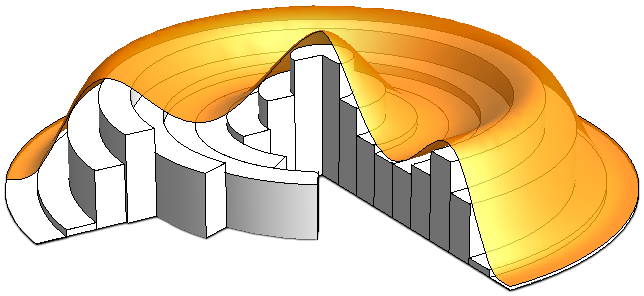
\includegraphics[width=0.5\textwidth]{./applications_integrals/shells.png}
	\caption{\hyperref{https://en.wikipedia.org/wiki/Shell\_integration}{}{}{Wikipedia - Shell Integration}}
\end{figure}


Each cylindrical shell will have a radius $r(x)$, a height $h(x)$, and a thickness $\d{x}$, meaning a volume of $2\pi r(x)h(x)\d{x}$.
\begin{equation*}
	V = 2\pi\int_{a}^{b}{r(x)h(x)\d{x}}.
\end{equation*}

\begin{example}
	Find the volume of the area bounded by the $y$-axis, $y=4-x^2$, and $y=x$ revolved around the $y$-axis.
\end{example}
\begin{answer}
	Each shell's height is parallel to the axis of rotation.
	In this case that's the distance between the two curves.
	\begin{equation*}
		h(x) = 4-x^2-x \text{ and } r(x)=x.
	\end{equation*}
	
	The two curves intersect at $x=\frac{-1+\sqrt{17}}{2}$.
	Finding the volume,
	\begin{align*}
		V &= 2\pi\int_{0}^{\frac{-1+\sqrt{17}}{2}}{x(4-x^2-x)\d{x}} \\
		&= 2\pi\left(-\frac{x^4}{4}-\frac{x^3}{3}+2x^2\right)\biggr\rvert_{0}^{\frac{-1+\sqrt{17}}{2}} \\
		&= \frac{\pi}{12}\left(121-17\sqrt{17}\right).
	\end{align*}
\end{answer}

\begin{example}
	Find the volume of the area bounded by the $x$-axis and the curve $y=(x-1)^2(x-2)^2$ rotated about the $y$-axis.
\end{example}
\begin{answer}
	The height of the shell is parallel to the $y$-axis.
	In this case it's exactly equal to the value of the bounding curve.
	\begin{equation*}
		h(x)=(x-1)^2(x-2)^2 \text{ and } r(x)=x.
	\end{equation*}
	
	Finding the volume,
	\begin{align*}
		V &= 2\pi\int_{1}^{2}{x(x-1)^2(x-2)^2\d{x}} \\
		&= 2\pi\left(\frac{x^6}{6}-\frac{6x^5}{5}+\frac{13x^4}{4}-4x^3+2x^2\right)\biggr\rvert_{1}^{2} \\
		&= \frac{\pi}{10}.
	\end{align*}
\end{answer}

\subsubsection{Other Axes of Rotation}
Although rotating about the $x$ and $y$ axes are the most common, the methods we have here apply to rotating about any axis parallel to the $x$ or $y$ axis.
The includes any lines of the form $y=k$ or $x=k$ where $k$ is some constant. \\


One valid approach is simply to rewrite the equations for your bounding curves by shifting them such that your axis of rotation is the $x$ or $y$ axis.
However, it's often more convenient to not rewrite the equations and simply apply the methods.

\begin{example}
	Find the volume of the solid generated by rotating the region in the first quadrant bounded by $y=x^2$ and $y=2x$ about the line $x=-2$.
\end{example}
\begin{answer}
	We can use the washer method (although shells also works).
	Since we're rotating about a line parallel to the $y$-axis, we'll have to rewrite our equations in the form $x=\ldots$.
	\begin{equation*}
		x = \sqrt{y} \text{ and } x = \frac{y}{2}.
	\end{equation*}
	
	The inner radius is given by the distance from $x=-2$ to $x=y/2$, and the outer radius is given by the distance from $x=-2$ to $x=\sqrt{y}$.
	The curves intersect at $y=0$ and $y=4$.
	\begin{align*}
		r(x) = 2 + \frac{y}{2} &\text{ and } R(x) = 2 + \sqrt{y} \\
		V &= \pi\int_{0}^{4}{(2+\sqrt{y})^2-\left(2+\frac{y}{2}\right)^2\d{y}} \\
		&= \pi\int_{0}^{4}{\left(4\sqrt{y}-y-\frac{y^2}{4}\right)\d{y}} \\
		&= 8\pi.
	\end{align*}
\end{answer}

\begin{example}
	Find the volume of the solid generated by rotating the region bounded by $y=x^2$ and $y=x+2$ about the line $x=3$.
\end{example} 
\begin{answer}
	We can use the shells method.
	Our height is simply the difference in $y$ values between the two curves.
	The radius is the distance between the lines $x=3$ and $x+2$.
	\begin{equation*}
		h(x) = x+2-x^2 \text{ and } r(x) = 3-x.
	\end{equation*}
	
	The curves intersect at $x=-1$ and $x=2$.
	Finding the volume,
	\begin{align*}
		V &= 2\pi\int_{-1}^{2}{(3-x)(x+2-x^2)\d{x}} \\
		&= 2\pi\left(\frac{x^4}{4}-\frac{4x^3}{3}+\frac{x^2}{2}+6x\right)\biggr\rvert_{-1}^{2} \\
		&= \frac{45\pi}{2}.
	\end{align*}
\end{answer}

\subsubsection{Surface Area}
Can apply the idea behind shell integration to derive a formula for surface area of a solid of rotation.
A cylindrical shell would have height $\d{s}$, which is given to us by the arc length formula, and radius $x$ or $y$, if the axis of rotation is the $y$ or $x$ axis respectively.
\begin{align*}
	S &= \begin{cases}
		2\pi\int{y\d{s}} & \text{Rotation about $x$-axis} \\
		2\pi\int{x\d{x}} & \text{Rotation about the $y$-axis}
	\end{cases} \\
	& \text{where } \\
	\d{s} &= \begin{cases}
		\sqrt{1+\left(\dd{y}{x}\right)^2}\d{x} & y=f(x) \\
		\sqrt{1+\left(\dd{x}{y}\right)^2}\d{y} & x=g(y) \\
	\end{cases}.
\end{align*}

\begin{example}
	Find the surface area of a sphere with radius $r$.
\end{example}
\begin{answer}
	We can obtain a sphere by rotating $y=\sqrt{r^2-x^2}, -r\leq x\leq r$ about the $x$-axis.
	\begin{align*}
		\dd{y}{x} &= \frac{-x}{\sqrt{r^2-x^2}} \\
		\left(\dd{y}{x}\right)^2 &= \frac{x^2}{r^2-x^2} \\
		S &= 2\pi\int_{-r}^{r}{y\sqrt{1+\frac{x^2}{r^2-x^2}}\d{x}} \\
		&= 2\pi\int_{-r}^{r}{\sqrt{r^2-x^2}\frac{r}{\sqrt{r^2-x^2}}\d{x}} \\
		&= 2\pi\int_{-r}^{r}{r\d{x}} \\
		&= 4\pi r^2.
	\end{align*}
\end{answer}
\section{Differential Equations}
Differential equations are equations, or sometimes systems of equations where we are given how a function relates to its derivatives and would like to find satisfying functions or families of functions.
Differential equations land themselves well to modeling real-world phenomena and are still an area of active mathematical study.
We'll see some very basic differential equations and how what we've learned about integrals can be used to solve them.

\subsection{Separable Differential Equations}
If we can break up a first-order (just involving a first derivative) ordinary differential equation into the following form,
\begin{equation*}
	\dd{y}{x} = f(x)g(y)
\end{equation*}
then we say the differential equation is separable and may be able to be solved using a technique called separation of variables.
The steps to solve a separable differential equation are:
\begin{enumerate}
	\item Write the equation in differential form (i.e using $\dd{y}{x}$)
	\item Separate the variables ($\frac{\d{y}}{g(y)}=f(x)\d{x}$)
	\item Integrate both sides
	\item Solve for $y$ in terms of $x$, if possible
	\item Find the general solution
	\item Find a particular solution, given any initial conditions
\end{enumerate}

\begin{example}
	Solve the following differential equation.
	\begin{equation*}
		\dd{y}{x} = (xy)^2, y(1)=1.
	\end{equation*}
\end{example}
Separating and integrating,
\begin{align*}
	\dd{y}{x} &= (xy)^2 = x^2y^2 \\
	\frac{\d{y}}{y^2} &= x^2\d{x} \\
	\frac{1}{y} &= \frac{x^3}{3} + C. \\
\end{align*}
\indent
Solving for $C$,
\begin{align*}
	\frac{-1}{1} &= \frac{1^3}{3} + C \\
	C &= \frac{-4}{3}.
\end{align*}
\indent
Solving for $y$,
\begin{align*}
	\frac{-1}{y} &= \frac{x^3}{3} - \frac{4}{3} \\
	y &= \frac{-3}{x^3 - 4}.
\end{align*}

\subsubsection{Exponential Growth \& Decay}
We can use differential equations to model growth and decay.

\begin{example}
	Imagine we have some money in a bank account earning interest.
	The more money in the bank, the more the more the account will receive in interest.
	So, the rate of growth of the account value is proportional to the current account value.
	In the language of differential equations,
	\begin{equation*}
		\dd{y}{t} = ky.
	\end{equation*}
	where $k$ is some constant of proportionality.
\end{example}
This equation is separable, so we'll try to solve it using separation of variables.
\begin{align*}
	\frac{\d{y}}{t} &= k\d{x} \\
	\ln{\abs{y}} &= kt + C \\
	\abs{y} &= Ce^{kt} \\
	y &= Ce^{kt} \\
	y(0) &= Ce^{k\cdot 0} = C \\
	y &= y_0e^{kt}.
\end{align*}
\noindent
This is exactly the equation for continually compounding interest: $y_0$ is the principle and $k$ is an interest rate.

\noindent
Note that $k$ could theoretically be negative, meaning the amount would decrease proportionally to the remaining amount.
\begin{example}
	The half-life of Pu-239 is 24360 years.
	Suppose that 10g of Pu-239 were released in a nuclear accident, how long would it take to decay to 1g?
\end{example}
Our "principle" is 10g.
We know that half-life follows the exponential decay differential equation, so it's modeled by $y = 10e^{kt}$.
We also know that $y(24360)=5$, which should give us enough information to solve for $k$.
\begin{align*}
	5 &= 10e^{k\cdot 24360} \\
	\frac{1}{2} &= e^{k\cdot 24360} \text{ (see the ``half" in half-life?)} \\
	\ln{\frac{1}{2}} &= 24360k \\
	-\ln{2} &= 24360k \\
	k &= \frac{-\ln{2}}{24360}. 
\end{align*}
\indent
We now can plug $k$ back into our equation to get the full model.
\begin{align*}
	y &= 10e^{\frac{-\ln{2}}{24360}t} \\
	&= 10\left(e^{\ln{2}}\right)^{\frac{-t}{24360}} \\
	&= 10\cdot2^{-\frac{-t}{24360}}.
\end{align*}
\indent
We can now plug in 1 for $y$ and solve for $t$
\begin{align*}
	1 &= 10\cdot2^{-\frac{t}{24360}} \\
	\frac{1}{10} &= 2^{-\frac{t}{24360}} \\
	\log_{2}{\frac{1}{10}} &= -\frac{t}{24360} \\
	\log_{2}{10} &= \frac{t}{24360} \\
	t &= 24360\log_{2}{10} \approx 80922\text{yr}.
\end{align*}
\indent
If you're familiar with half-life equations, this is exactly $t=t_{1/2}\log_{2}{\frac{N_0}{N_f}}$.

\subsubsection{Logistic Growth \& Decay}
Although our differential equations assuming that growth is proportional to amount work well for things like bank accounts, bacteria or radioactive particles that can grow and decay without limits, that model is a little too simplistic to model populations that are limited by resources.

\begin{example}
	Imagine that we have a population of animals in a forest.
	If the forest has lots of resources to support to animal population, then they can grow basically like normal.
	However, as the population grows, resources become more scarce, so population growth would slow down, or some of the population would starve.
	We can model this with the following differential equation.
	\begin{equation*}
		\dd{P}{t} = kP(M-P)
	\end{equation*}
	where $k$ is some constant of proportionality and $M$ is some maximum population before growth starts to decline.
\end{example}
This differential equation is also separable, so let's try to solve it.
\begin{align*}
	\dd{P}{t} &= kP(M-P) \\
	\frac{\d{P}}{P(M-P)} &= k\d{t} \\
	\d{P}\left(\frac{1/M}{P}+\frac{1/M}{M-P}\right) &= k\d{t} \text{ (using partial fractions)} \\
	\frac{1}{M}\left(\ln{\abs{P}} - \ln{\abs{M-P}}\right) &= kt + C \\
	\ln{\abs{\frac{P}{M-P}}} &= Mkt + C \\
	\frac{P}{M-P} &= Ce^{Mkt} \text{ (b/c $P \geq 0$)} \\
	P &= CMe^{Mkt} - CPe^{Mkt} \\
	P\left(1+Ce^{Mkt}\right) &= CMe^{Mkt} \\
	P &= \frac{CMe^{Mkt}}{1+Ce^{Mkt}} \\
	&= \frac{M}{1+Ce^{-Mkt}}.
\end{align*}

\begin{figure}[H]
	\label{logistic}
	\centering
	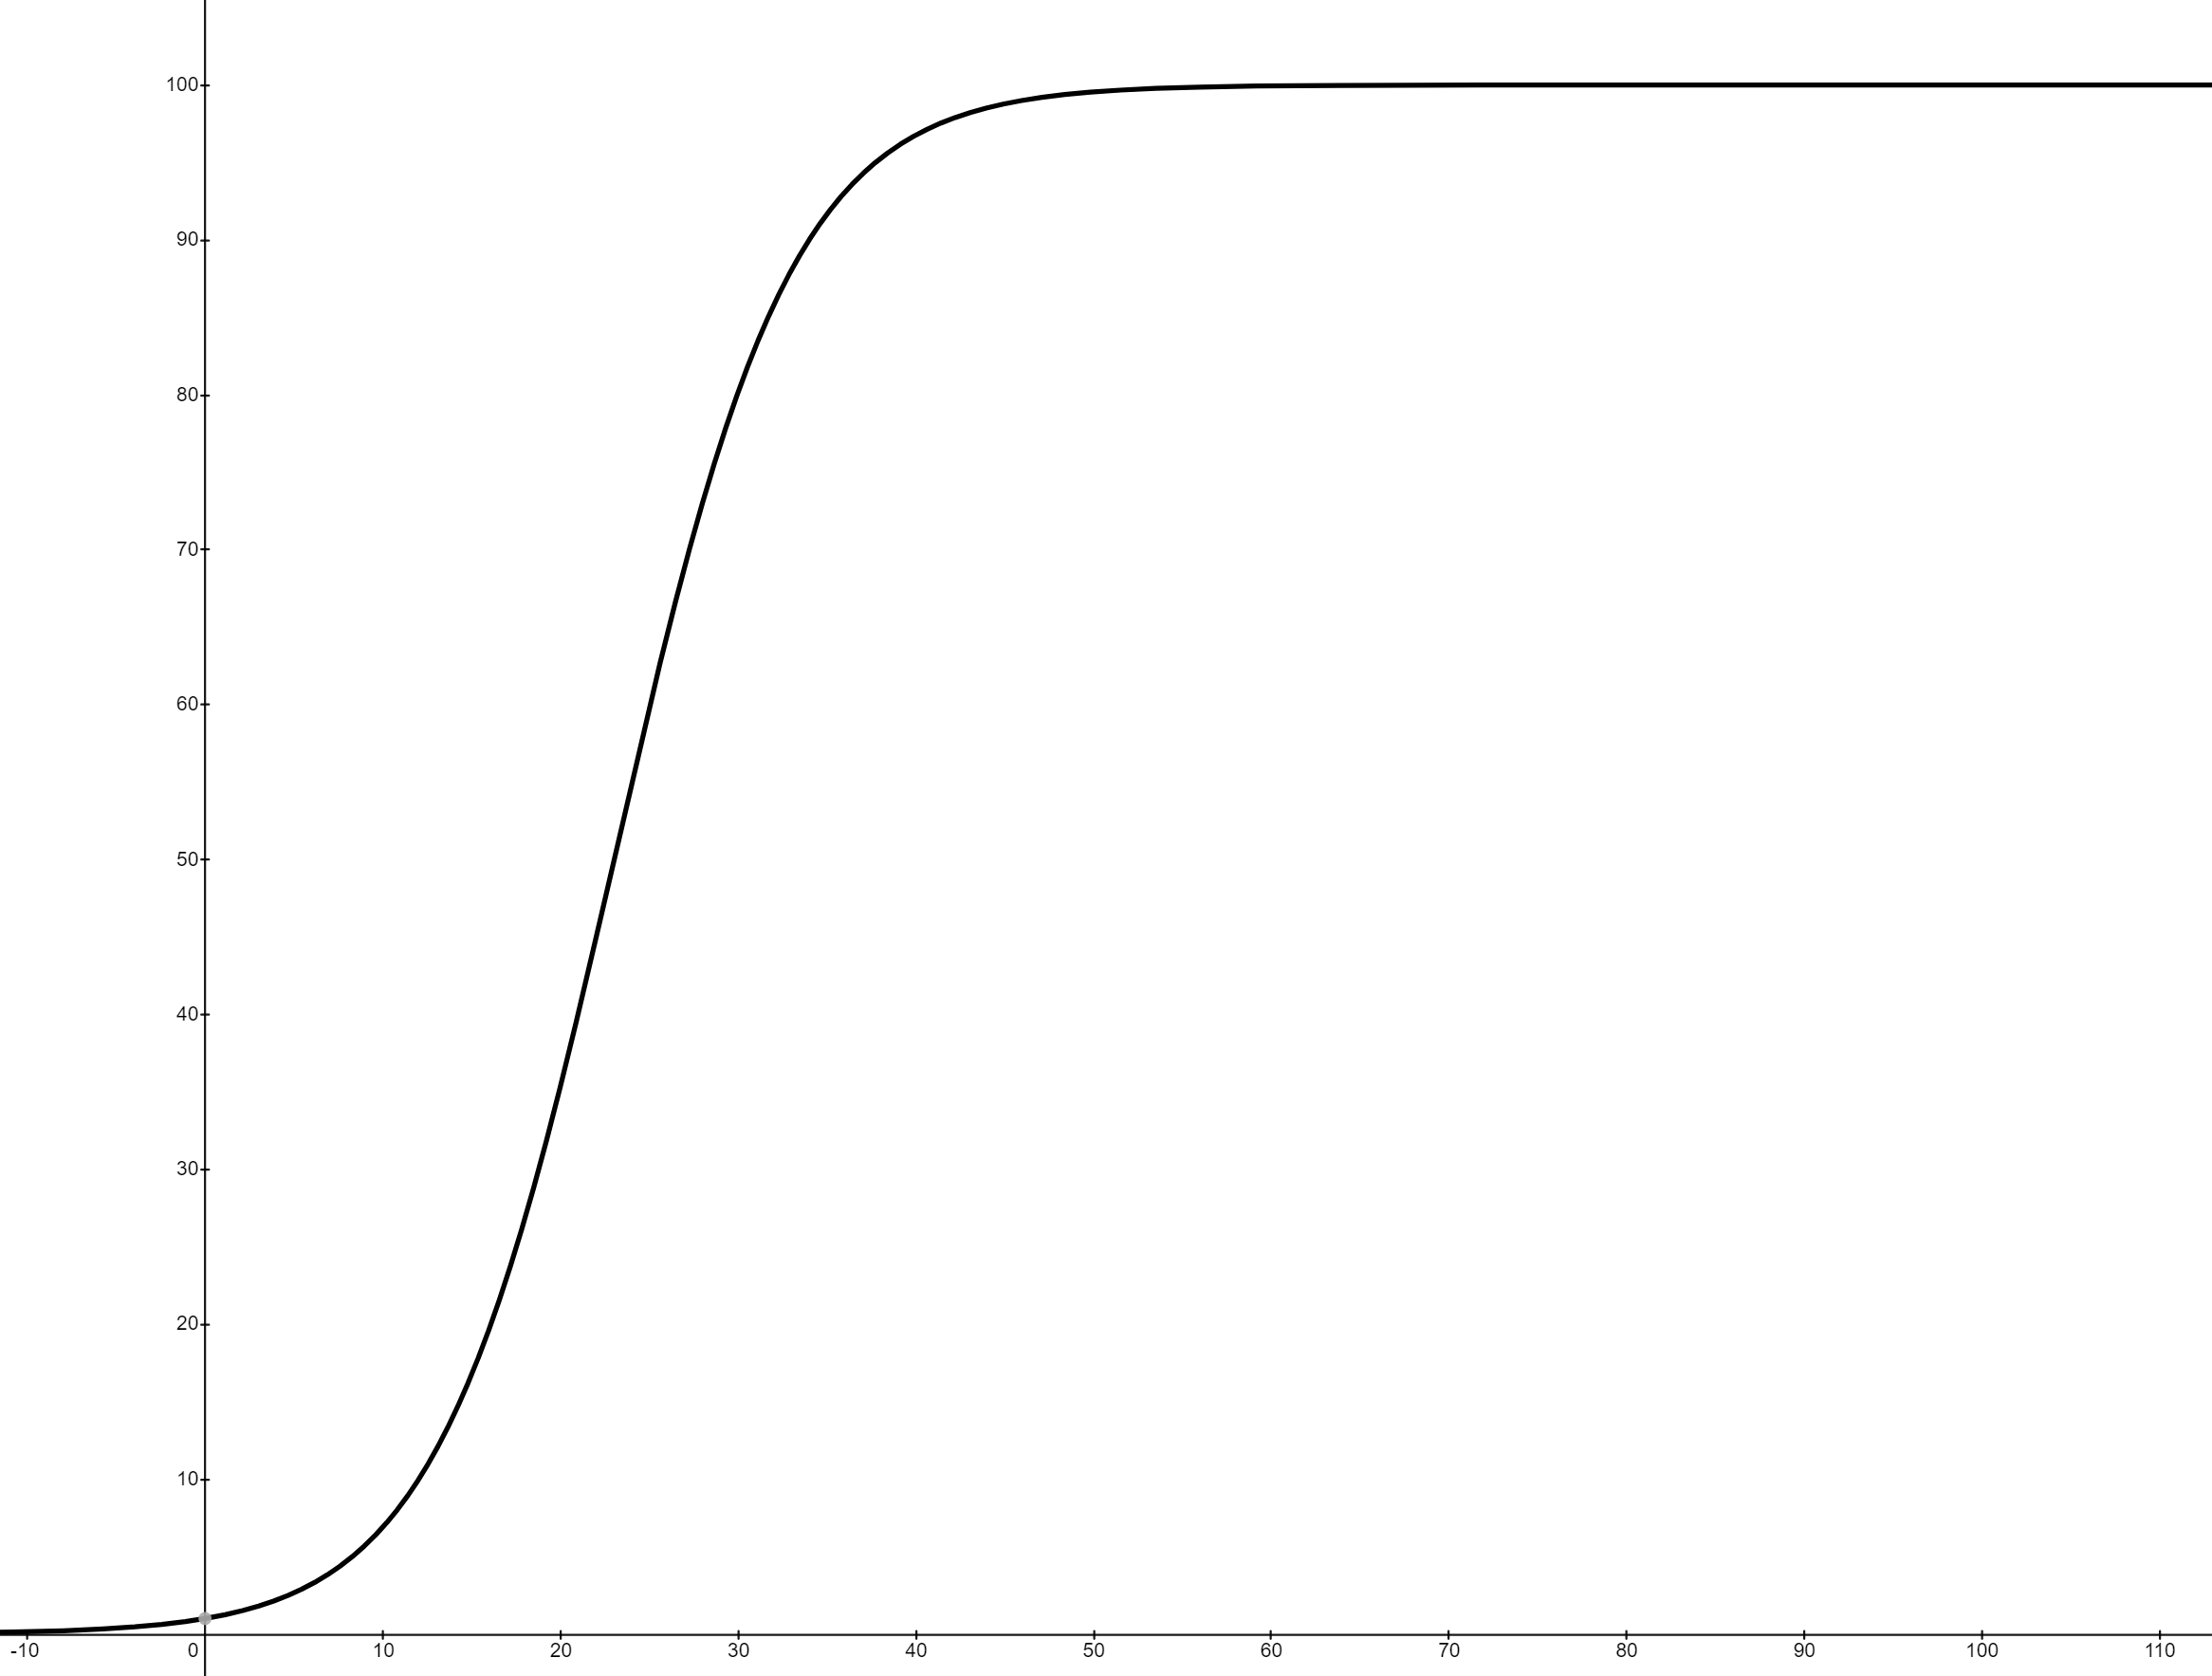
\includegraphics[width=0.5\textwidth]{./applications_integrals/logistic_growth.png}
	\caption{\hyperref{}{}{}{Logistic Growth}}
\end{figure}
\noindent
Looking at a graph of this function, we can see that it starts growing like an exponential curve but begins to flatten, obtaining a maximum value of $M$, which is called the carrying capacity.
The population is growing the fastest when $P=M/2$, which you can verify by finding the global maxima of $\dd{P}{t}$ using a first derivative test.

\subsection{Slope Fields \& Euler's Method}
Unfortunately, not all differential equations are as easy to solve as separable differential equations.
In fact, some are impossible to get nice, closed-form solutions.
\subsubsection{Slope Fields}
We may still be able to visualize what the graph of a solution might look like by drawing lines that have the same slope as a solution.
Any solution that passes through the points where we draw the sloped lines must be tangent to these lines, meaning a solution will follow the ``flow" of these lines.

\begin{figure}[H]
	\label{slope_field}
	\centering
	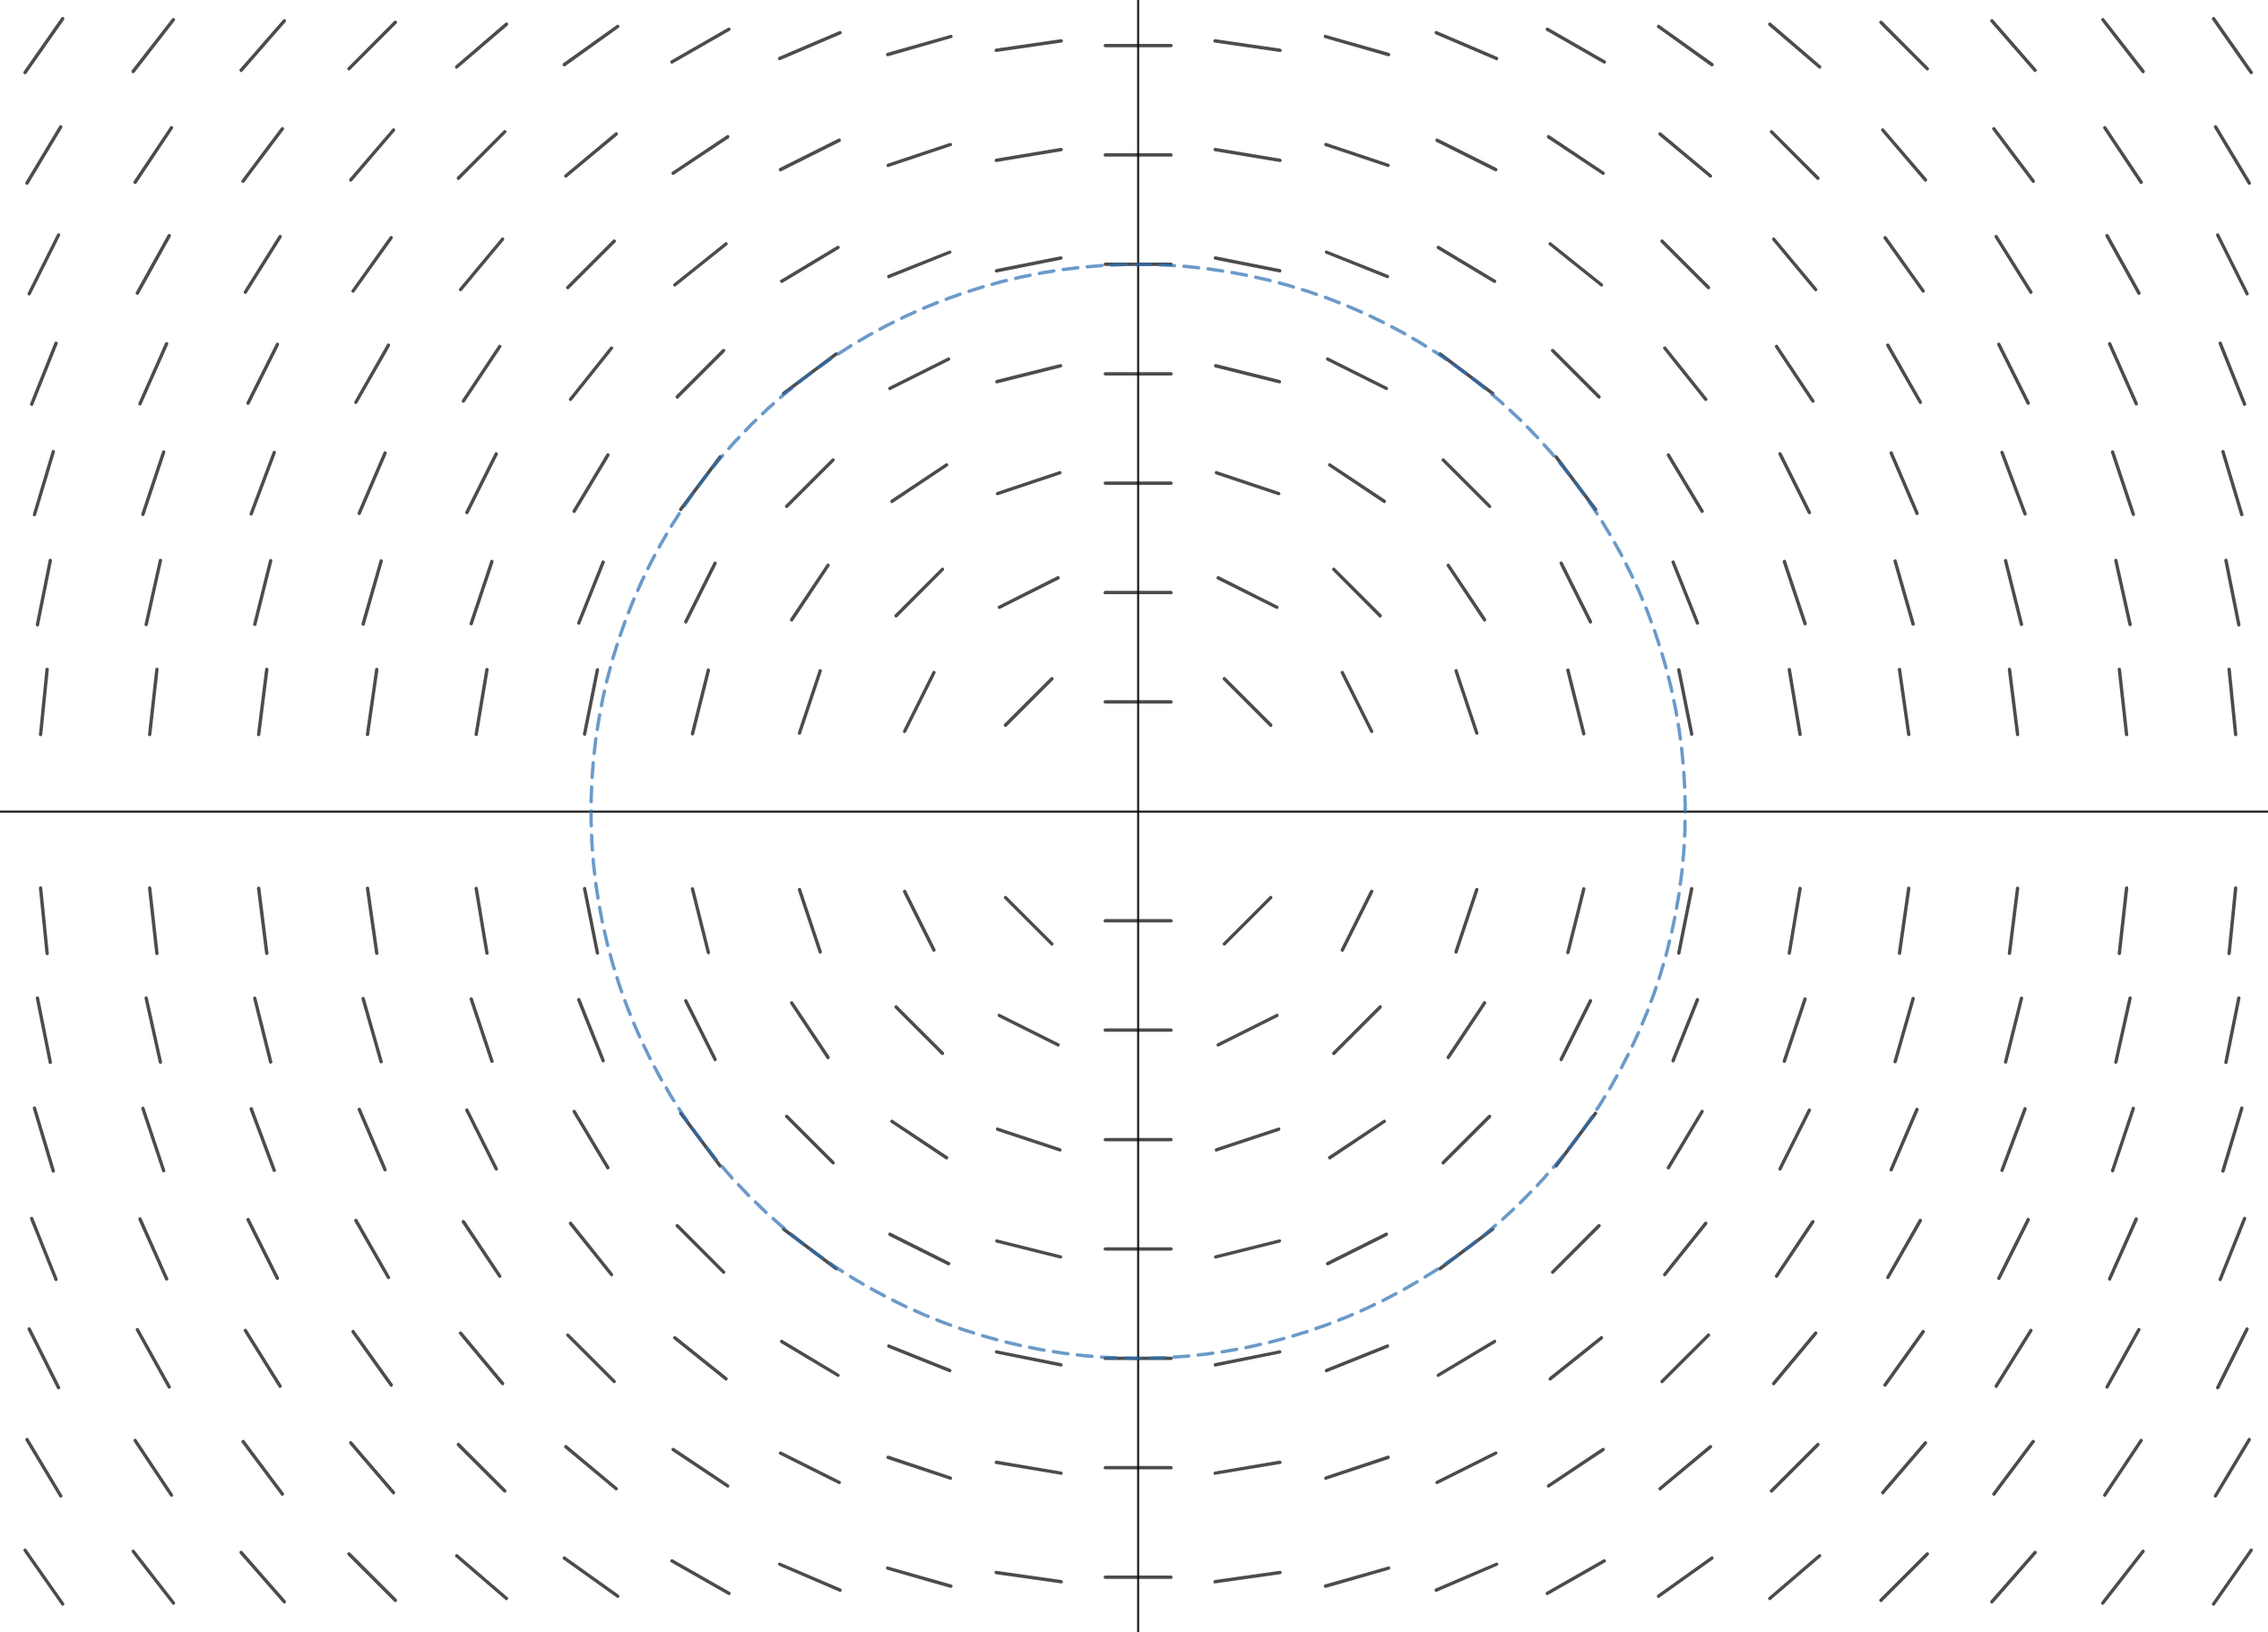
\includegraphics[width=0.75\textwidth]{./applications_integrals/slope_field.png}
	\caption{\hyperref{}{}{}{Slope field of $\dd{y}{x}=-x/y$ with a possible solution}}
\end{figure}

\subsubsection{Euler's Method}
If your differential equation also has an initial condition, you can start at the initial point and follow the slope field to find an approximate solution.
This is what Euler's Method tries to accomplish.
It can approximate the value of a solution at some $x$ value by starting at some point, usually given by the initial condition, and iteratively taking small steps of size $\Delta x$ in the direction determined by the slope field.
\begin{align*}
	x_{n+1} &= x_n + \Delta x \\
	y_{n+1} &= y_n + \Delta x\dd{y}{x}_{(x_n,y_n)}.
\end{align*}
\noindent
The smaller the steps, the more accurate the approximation.
\begin{figure}[H]
	\label{eulers_method}
	\centering
	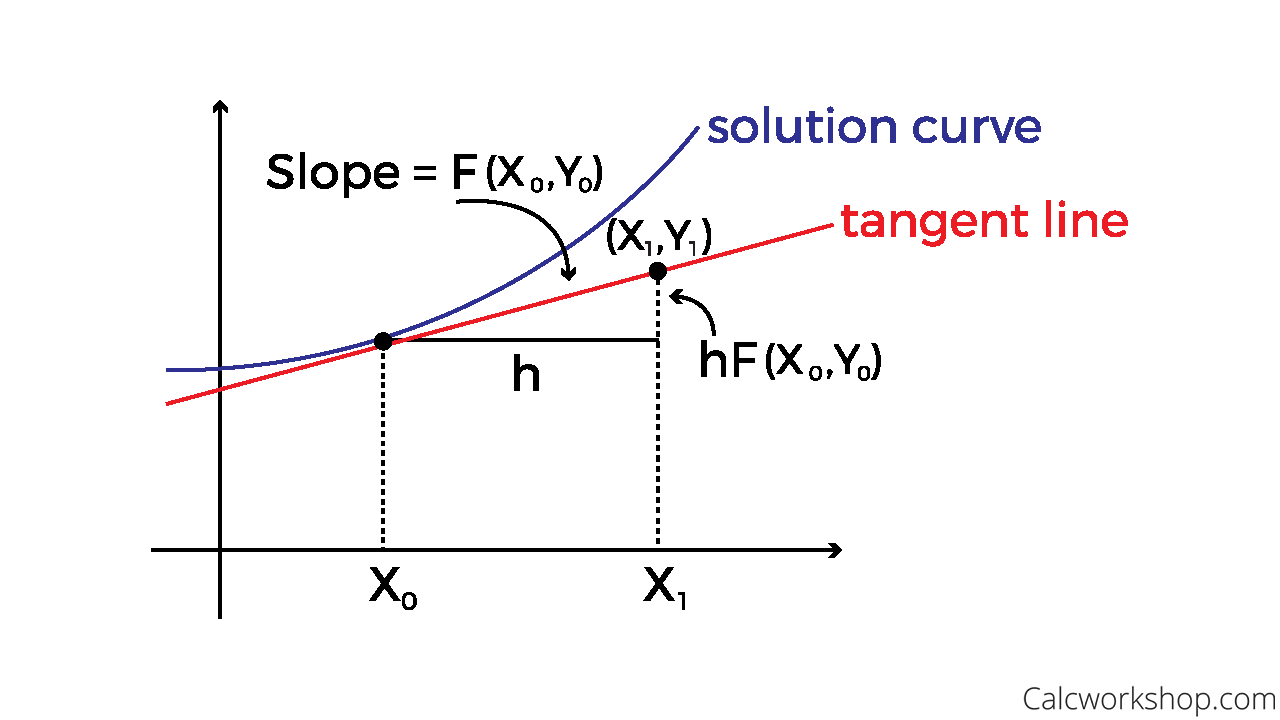
\includegraphics[width=0.55\textwidth]{./applications_integrals/Eulers-Approximation.png}
	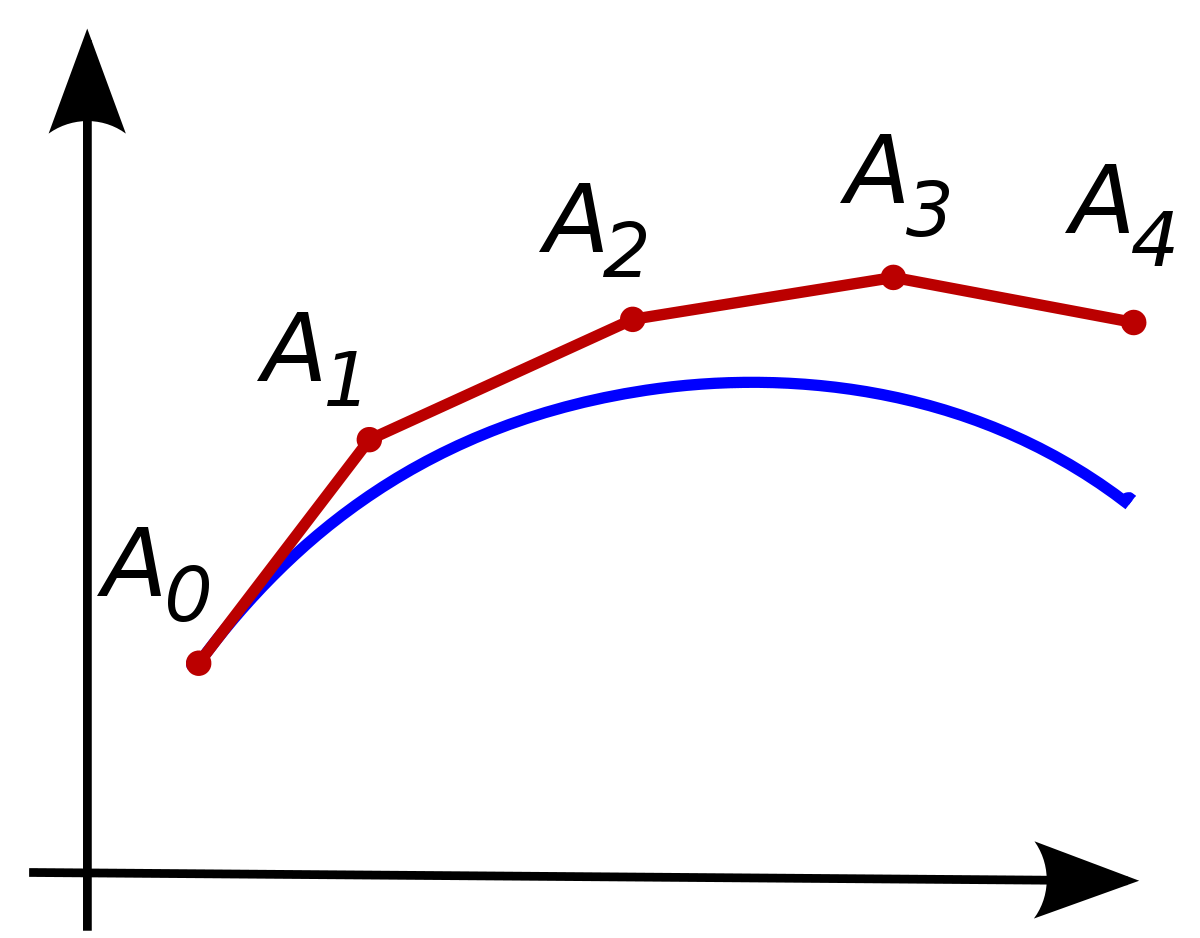
\includegraphics[width=0.35\textwidth]{./applications_integrals/Eulers-Approximation2.png}
	\caption{\hyperref{https://calcworkshop.com/first-order-differential-equations/eulers-method-table/}{}{}{Calc Workshop - Euler's Method};\hspace{5pt}\hyperref{https://en.wikipedia.org/wiki/Euler\_method}{}{}{Wikipedia - Euler Method}}
\end{figure}

\begin{example}
	Given that $\dd{y}{x}=3-x$ and $y(4)=2$, approximate the value of $y(5)$ using Euler's method with increments of $\Delta x = 0.25$.
\end{example}
\begin{table}[H]
\begin{center}
	\begin{tabular}{|c|c|c|c|c|}
		\hline
		$(x,y)$ & $\dd{y}{x}$ & $\Delta x$ & $\Delta y = \Delta x\dd{y}{x}$ & $(x+\Delta x, y+\Delta y)$ \\
		\hline
		$(4,2)$ & $-1$ & $0.25$ & $-0.25$ & $(4.25,1.75)$ \\
		\hline
		$(4.25,1.75)$ & $-1.25$ & $0.25$ & $-0.3125$ & $(4.5,1.4375)$ \\
		\hline
		$(4.5,1.4375)$ & $-1.5$ & $0.25$ & $-0.375$ & $(4.75,1.0625)$ \\
		\hline
		$(4.75,1.0625)$ & $-1.75$ & $0.25$ & $-0.4375$ & $(5,0.625)$ \\
		\hline
	\end{tabular}
\end{center}
\end{table}
\indent
So, Euler's Method yields an approximate\footnote{The actual value of the solution is $(5,0.5)$, so not too far off.} value of $(5,0.625)$.
		\chapter{Parametric, Vector, \& Polar Functions}

\section{Parametric \& Vector Functions}
Up to this point, almost all the graphs we have worked with have been of the form $y=f(x)$, defining the $y$ coordinate in terms of the $x$ coordinate.
These sorts of functions are limited in the types of graphs they can draw.
If we instead let both the $x$ and $y$ coordinates be defined in terms of another variable $t$, like $(x(t),y(t))$, then we can draw much more interesting graphs.
For example, a unit circle, which can't be defined with a single function $y=f(x)$, would be $(\cos{t}, \sin{t})$. \\

\noindent
We are always able to translate a function of the form $y=f(x)$ into a parametric function as $(t, f(t))$.
Sometimes, but not always, we are also able to translate parametric functions into $y$ as a function of $x$.

\begin{example}
	Given the following parametric function, find $y$ as a function of $x$.
	\begin{equation*}
		(\sqrt{t}, t-2).
	\end{equation*}
\end{example}
Squaring both sides of the $x$ equation,
\begin{equation*}
	x^2 = t.
\end{equation*}
\indent
Substituting our expressing for $t$ in terms of $x$ into the $y$ equation,
\begin{equation*}
	y = x^2 - 2.
\end{equation*}

\subsection{Vector Functions}
Vector and parametric functions are essentially the same thing.
In fact, in multivariable calculus, we drop the idea of parametric functions almost completely and exclusively talk about vector-valued functions.
Both can graph the exact same functions.
Visually, you might imagine an arrow rooted at the origin tracing out the graph of a vector function. 
You're more likely to see vector functions written in the following form
\begin{equation*}
	\vec{r}(t) = \langle x(t), y(t) \rangle.
\end{equation*}
\noindent
All the normal vector operations, like addition and subtraction, scalar multiplication, and dot products work exactly the same.
If we think of $\vec{r}(t)$ as a position function,
\begin{align*}
	\textbf{Velocity: }& \vec{v}(t) = \vec{r^\prime}(t) = \langle x^\prime(t), y^\prime(t) \rangle \\
	\textbf{Speed: }& \abs{\vec{v}(t)} = \sqrt{\left(x^\prime(t)\right)^2 + \left(y^\prime(t)\right)^2} \\
	\textbf{Acceleration: }& \vec{a}(t) = \vec{v^\prime}(t) = \langle x^{\prime\prime}(t), y^{\prime\prime}(t) \rangle \\
	\textbf{Direction: }& \frac{\vec{t}(t)}{\abs{\vec{v}(t)}} \\
\end{align*}

\subsection{Slope \& Concavity}
Just like with functions like $y=f(x)$, we can find the slope and concavity of parametric functions using first and second derivatives respectively.
We just apply the chain rule.
\begin{align*}
	\dd{y}{x} &= \frac{\dd{y}{t}}{\dd{x}{t}} \\
	\dd{^2y}{x^2} &= \dd{y^\prime}{x} = \frac{\d{y^\prime}/\d{t}}{\d{x}/\d{t}}.
\end{align*}

\begin{example}
	Consider the following parametric function:
	\begin{equation*}
		(t^2-5, 2\sin{t}), 0\leq t\leq\pi.
	\end{equation*}
	Find the first and second derivatives of $y$ with respect to $x$.
\end{example}
Differentiating both $x$ and $y$ with respect to $t$,
\begin{align*}
	x^\prime(t) &= 2t \\
	y^\prime(t) &= 2\cos{t} \\
	\dd{y}{x} &= \frac{2\cos{t}}{2t} = \frac{\cos{t}}{t}.
\end{align*}
Finding the derivative of $y^\prime$ with respect to $t$,
\begin{align*}
	\dd{}{t}y^\prime &= \dd{}{t}\frac{\cos{t}}{t} \\
	&= \frac{-t\sin{t}-\cos{t}}{t^2} \\
	\dd{^2y}{x^2} &= \frac{\d{y^\prime}/\d{t}}{\d{x}/\d{t}} \\
	&= \frac{\frac{-t\sin{t}-\cos{t}}{t^2}}{2t} \\
	&= -\frac{t\sin{t}+\cos{t}}{2t^3}.
\end{align*}

\subsection{Arc Length}
Remember that we had the following formula for $\d{s}$ when deriving arc length.
\begin{equation*}
	\d{s} = \sqrt{\left(\d{x}\right)^2 + \left(\d{y}\right)^2}.
\end{equation*}
Since we now have $x$ and $y$ as functions of $t$, we can rewrite this formula to get a formula for arc length of a parametric function.
\begin{align*}
	\d{s} &= \sqrt{\left(\dd{x}{t}\right)^2 + \left(\dd{y}{t}\right)^2}\d{t} \\
	s &= \int_{a}^{b}{\sqrt{\left(\dd{x}{t}\right)^2 + \left(\dd{y}{t}\right)^2}\d{t}}.
\end{align*}
\noindent
When talking about vector-valued functions or working in a more physics-based context, you might hear the term ``distance traveled" instead of arc length and see the following formula.
They are equivalent ideas.
\begin{equation*}
	s = \int_{a}^{b}{\abs{\vec{v}(t)}\d{t}}.
\end{equation*}

\begin{example}
	A circle of radius $r$ is defined parametrically as
	\begin{equation*}
		(r\cos{t}, r\sin{t}), 0 \leq t \leq 2\pi.
	\end{equation*}
	Use this definition to find its circumference.
\end{example}
\begin{align*}
	\dd{x}{t} &= -r\sin{t} \\
	\left(\dd{x}{t}\right)^2 &= r^2\sin^2{t} \\
	\dd{y}{t} &= r\cos{t} \\
	\left(\dd{y}{t}\right)^2 &= r^2\cos^2{t} \\
	C &= \int_{0}^{2\pi}{\sqrt{r^2\sin^2{t}+r^2\cos^2{t}}\d{t}} \\
	&= \int_{0}^{2\pi}{r\sqrt{\sin^2{t}+\cos^2{t}}\d{t}} \\
	&= \int{0}^{2\pi}{r\d{t}} \\
	&= 2\pi r.
\end{align*}
\section{Polar Functions}
\subsection{Polar Coordinates}
Up to this point, we've mostly described points in the plane by listing two numbers: the distance along the $x$-axis and the distance along the $y$-axis.
This description, called ``rectangular coordinates" is pretty simple and has the advantage that every pair of coordinates describes a unique point on the plane. \\


However, we could instead describe points in the plane with two numbers $(r,\theta)$, where $r$ is the point's distance from the origin and $\theta$ is the point's angle of inclination.
This system is more suited to describing points related to trig functions.
For example the point at $x=\cos{\frac{\pi}{4}}$ and $y=\sin{\frac{\pi}{4}}$ is $\left(\frac{\sqrt{2}}{2},\frac{\sqrt{2}}{2}\right)$ in rectangular coordinates but $\left(1,\frac{\pi}{4}\right)$ in polar coordinates. \\


Note that unlike rectangular coordinates, multiple pairs of numbers can describe the same point.
For example $\left(1,0\right)$ is the same point as $\left(1,2\pi\right)$ is the same point as $\left(1,-2\pi\right)$ is the same point as $\left(1,4\pi\right)$. \\


We can easily convert between polar and rectangular coordinates.
\begin{align*}
	\left(r,\theta\right) \text{polar} &= \left(r\cos{\theta}, r\sin{\theta}\right) \text{rectangular} \\
	\left(x,y\right) \text{rectangular} &= \left(\sqrt{x^2+y^2}, \arctan{\frac{y}{x}}\right) \text{polar}.
\end{align*}

\subsection{Polar Functions}
Polar functions are written in the form $r = f(\theta)$.
Using our polar coordinate conversion formulas, we can convert any polar function to a parametric function.
\begin{align*}
	x(\theta) &= r\cos{\theta} = f(\theta)\cos{\theta} \\
	y(\theta) &= r\sin{\theta} = f(\theta)\sin{\theta}.
\end{align*}

Now we can use our parametric function formulas to get $\dd{y}{x}$.
\begin{equation*}
	\dd{y}{x} = \frac{\d{y}/\d{\theta}}{\d{x}/\d{\theta}}.
\end{equation*}

\begin{example}
	A cardioid is defined by $r=1-\cos{\theta}, 0 \leq \theta \leq 2\pi$.
	Find $\dd{y}{x}$.
\end{example}
\begin{answer}
	\begin{align*}
		x(\theta) &= \left(1-\cos{\theta}\right)\cos{\theta} \\
		\dd{x}{\theta} &= \sin{(2\theta)} - \sin{\theta} \\
		y(\theta) &= \left(1-\cos{\theta}\right)\sin{\theta} \\
		\dd{y}{\theta} &= \cos{\theta} - \cos{(2\theta)} \\
		\dd{y}{x} &= \frac{\cos{\theta} - \cos{(2\theta)}}{\sin{(2\theta)} - \sin{\theta}} \\
		&= \tan{\frac{3\theta}{2}}.
	\end{align*}
\end{answer}

\subsubsection{Area Enclosed}
When a polar function is changed by $\d{\theta}$, it sweeps out an circular sector.

\begin{figure}[H]
	\label{polar_area}
	\centering
	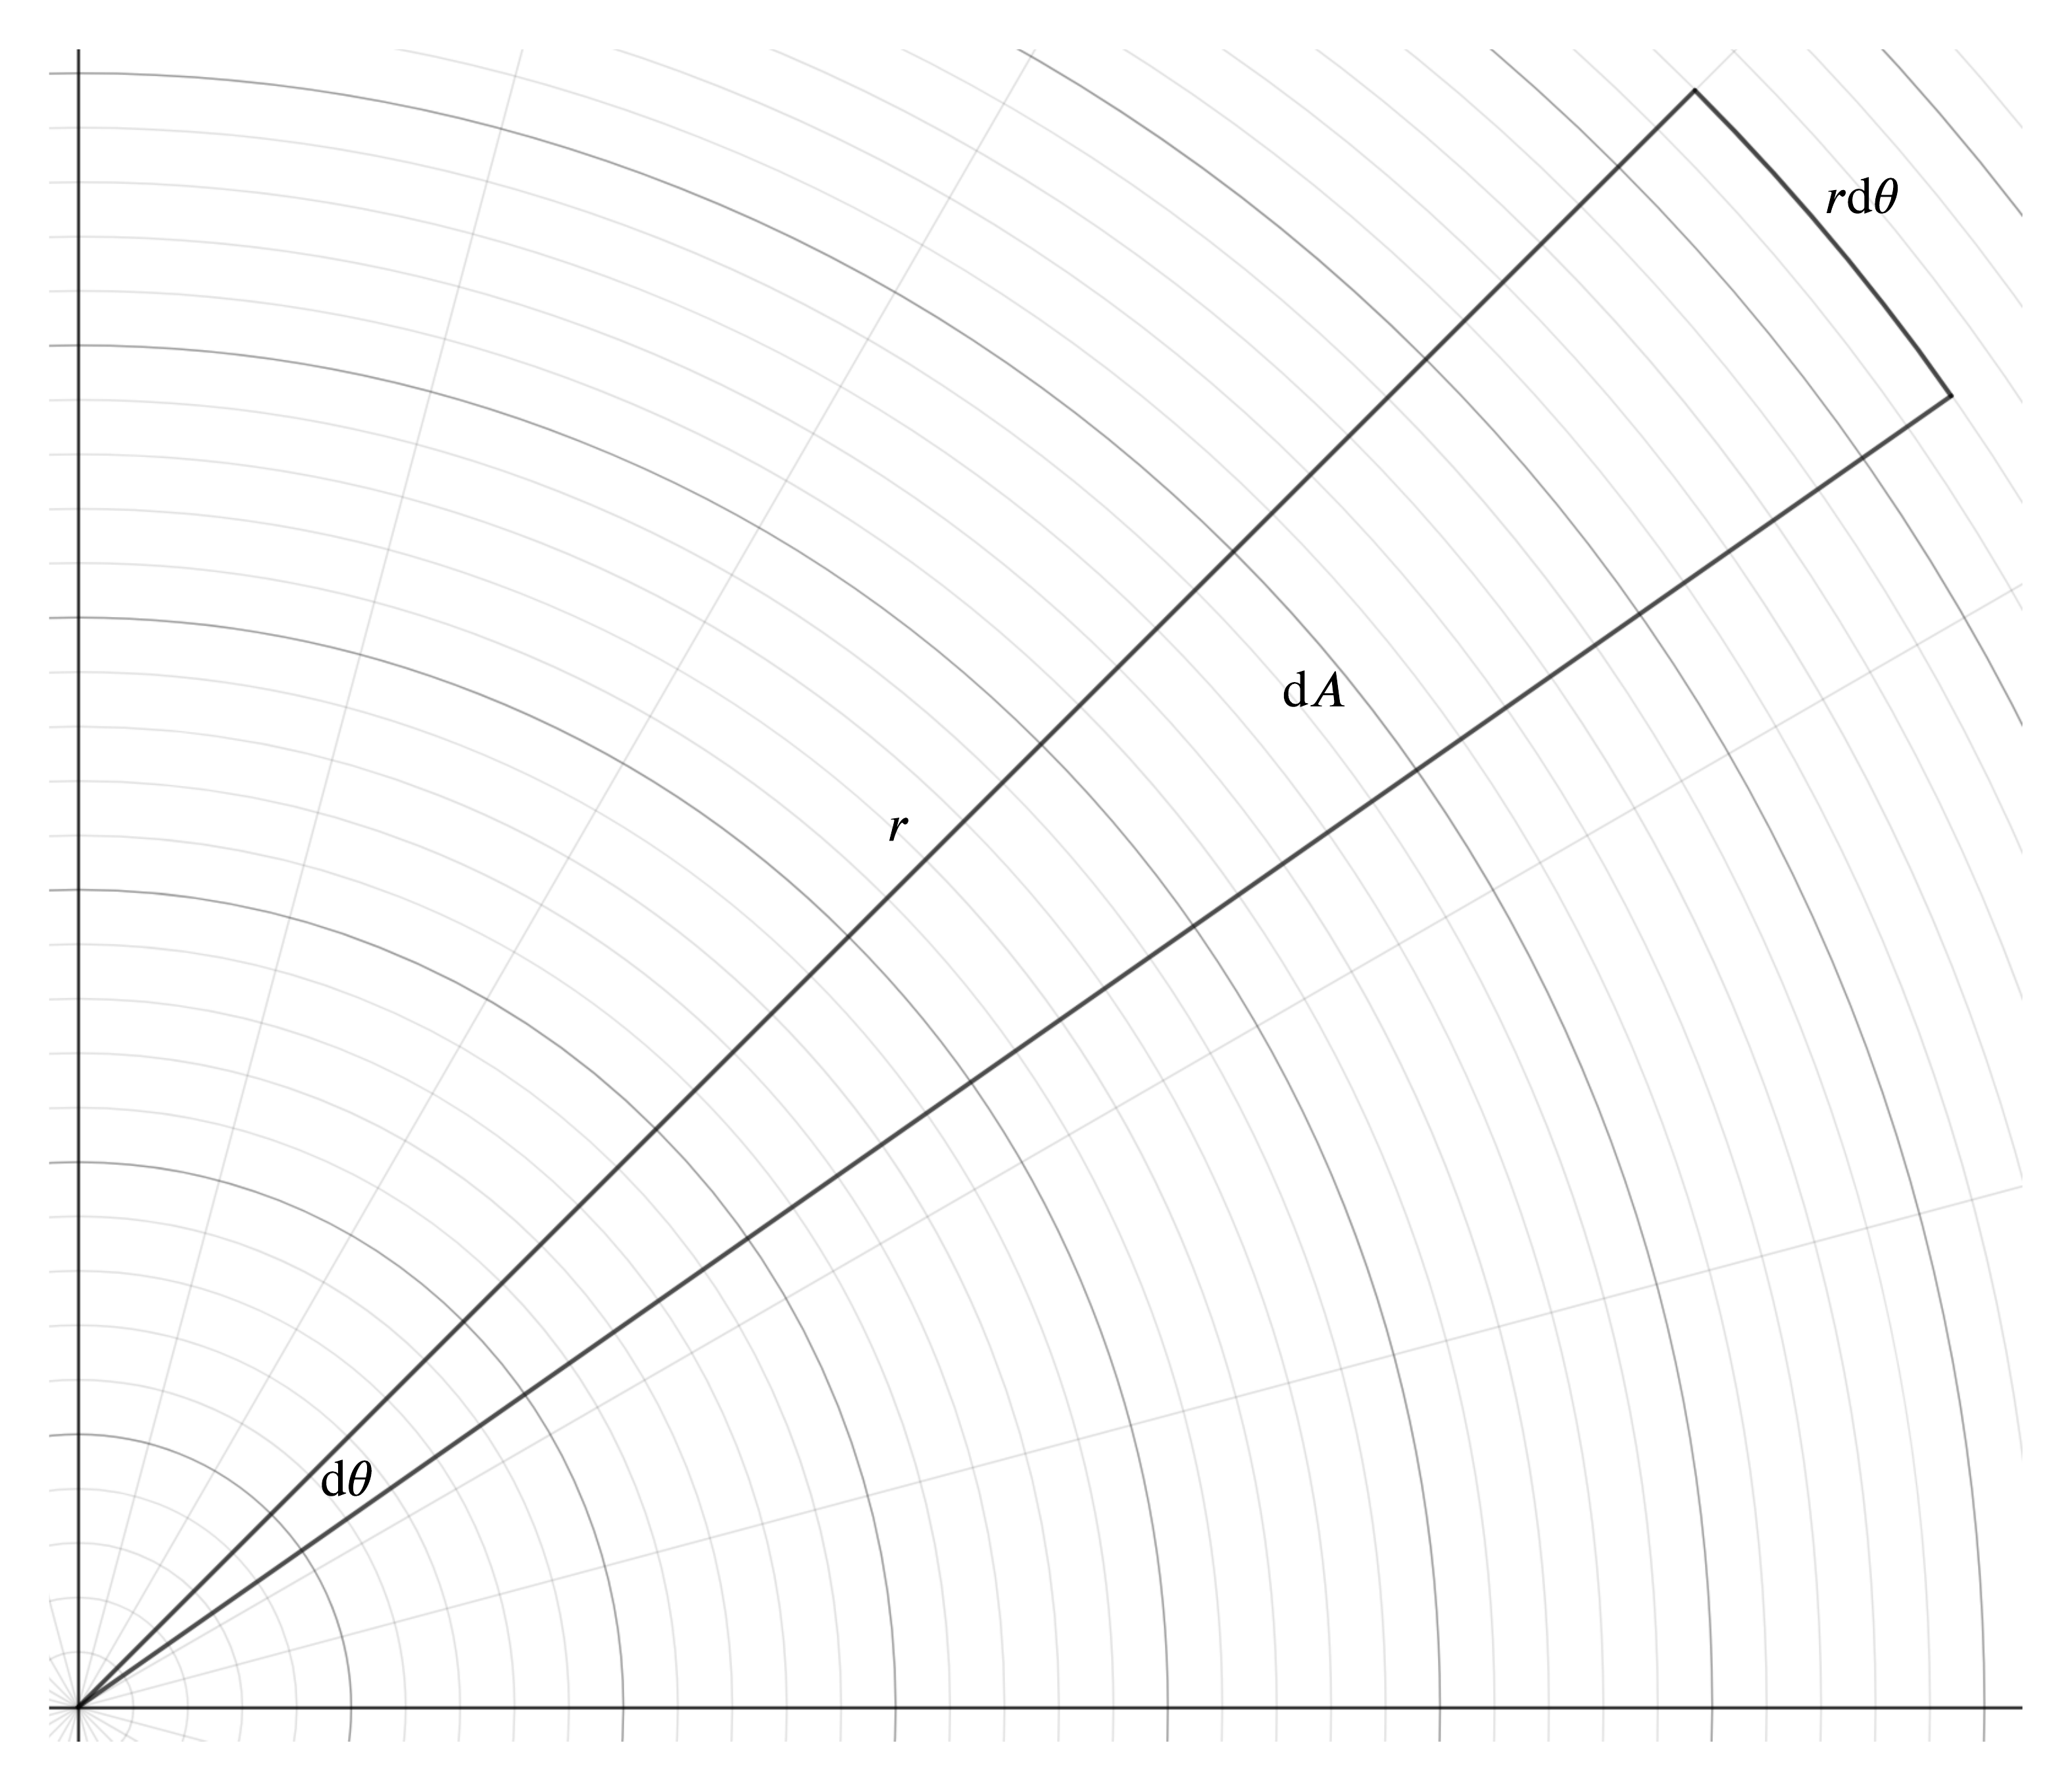
\includegraphics[width=0.66\textwidth]{./parametric_vector_polar/polar_area.png}
	\caption{\hyperref{}{}{}{Polar Area}}
\end{figure}

This circular sector has area $\d{A} = \frac{\d{\theta}}{2}r^2$.
Integrating $\d{A}$ for $\alpha \leq \theta \leq \beta$,
\begin{equation*}
	A = \int_{\alpha}^{\beta}{\frac{1}{2}r^2\d{\theta}} = \int_{\alpha}^{\beta}{\frac{1}{2}f^2(\theta)\d{\theta}}.
\end{equation*}

\begin{example}
	Find the area inside the smaller loop of the lima\c{c}on $r=2\cos{\theta}+1$.
\end{example}
\begin{answer}
	First, we need to find our bounds on $\theta$.
	We know that the small loop begins and ends when $r=0$.
	\begin{align*}
		0 &= 2\cos{\theta}+1 \\
		-\frac{1}{2} &= \cos{\theta} \\
		\theta &= \frac{\pi}{3}, \frac{4\pi}{3}.
	\end{align*}
	
	Now that we have our bounds, we can integrate.
	\begin{align*}
		A &= \int_{2\pi/3}^{4\pi/3}{\frac{1}{2}\left(2\cos{\theta}+1\right)^2\d{\theta}} \\
		&= \frac{1}{2}\left(\int_{\frac{2\pi}{3}}^{\frac{4\pi}{3}}4\cos^{2}\left(\theta\right)\d{\theta}+4\int_{\frac{2\pi}{3}}^{\frac{4\pi}{3}}\cos\left(\theta\right)\d{\theta}+\int_{\frac{2\pi}{3}}^{\frac{4\pi}{3}}\d{\theta}\right) \\
		&= \int_{\frac{2\pi}{3}}^{\frac{4\pi}{3}}\left(1+\cos\left(2\theta\right)\right)\d{\theta}+2\int_{\frac{2\pi}{3}}^{\frac{4\pi}{3}}\cos\left(\theta\right)\d{\theta}+\frac{1}{2}\int_{\frac{2\pi}{3}}^{\frac{4\pi}{3}}\d{\theta} \\
		&= \int_{\frac{2\pi}{3}}^{\frac{4\pi}{3}}\cos\left(2\theta\right)\d{\theta}+2\int_{\frac{2\pi}{3}}^{\frac{4\pi}{3}}\cos\left(\theta\right)\d{\theta}+\frac{3}{2}\int_{\frac{2\pi}{3}}^{\frac{4\pi}{3}}\d{\theta} \\
		&= \frac{1}{2}\sin\left(2\theta\right)+2\sin\left(\theta\right)+\frac{3}{2}\theta \biggr\rvert_{2\pi/3}^{4\pi/3} \\
		&= \left(\frac{1}{2}\sin\left(\frac{8\pi}{3}\right)+2\sin\left(\frac{4\pi}{3}\right)+\frac{3}{2}\frac{4\pi}{3}\right)-\left(\frac{1}{2}\sin\left(\frac{4\pi}{3}\right)+2\sin\left(\frac{2\pi}{3}\right)+\frac{3}{2}\frac{2\pi}{3}\right) \\
		&= \left(\frac{\sqrt{3}}{4}-\sqrt{3}+2\pi\right)-\left(-\frac{\sqrt{3}}{4}+\sqrt{3}+\pi\right) \\
		&= \frac{\sqrt{3}}{2}-2\sqrt{3}+\pi \\
		&= \pi-\frac{3\sqrt{3}}{2}.
	\end{align*}
\end{answer}

\subsubsection{Area Between Curves}
The area between $r_1(\theta)$ and $r_2(\theta)$ is simply the difference between the areas.
\begin{equation*}
	A = \frac{1}{2}\int_{\alpha}^{\beta}{r_1^2(\theta)\d{\theta}} - \frac{1}{2}\int_{\alpha}^{\beta}{r_2^2(\theta)\d{\theta}} = \frac{1}{2}\int_{\alpha}^{\beta}{(r_1^2(\theta)-r_2^2(\theta))\d{\theta}}.
\end{equation*}

\begin{example}
	Find the area that lies inside the circle $r=1$ and outside the cardioid $r=1-\cos{\theta}$.
\end{example}
\begin{answer}
	To find the bounds, we need to find where these curves intersect.
	\begin{align*}
		1 &= 1-\cos{\theta} \\
		\cos{\theta} &= 0 \\
		\theta &= \frac{\pi}{2}, \frac{-\pi}{2}.
	\end{align*}
	
	Since we want the area inside of the circle and outside of the cardioid, our bounds are $\frac{-\pi}{2} \leq \theta \leq \frac{\pi}{2}$.
	We'll also have $r_1(\theta)$ be the circle and $r_2(\theta)$ be the cardioid, since we are effectively finding the area inside the circle and subtracting away the area that is also in the cardioid.
	\begin{align*}
		A &= \frac{1}{2}\int_{-\pi/2}^{\pi/2}{\left(1^2 - \left(1-\cos{\theta}\right)^2\right)\d{\theta}} \\
		&= \frac{1}{2}\int_{\frac{-\pi}{2}}^{\frac{\pi}{2}}\left(2\cos\left(\theta\right)-\cos^{2}\theta\right)\d{\theta} \\
		&= \frac{1}{2}\int_{\frac{-\pi}{2}}^{\frac{\pi}{2}}\left(2\cos\left(\theta\right)-\frac{1+\cos\left(2\theta\right)}{2}\right)\d{\theta} \\
		&= \frac{1}{2}\left(2\sin\left(\theta\right)-\frac{\theta}{2}-\frac{\sin\left(2\theta\right)}{4}\right) \biggr\rvert_{\frac{-\pi}{2}}^{\frac{\pi}{2}} \\
		&= \frac{1}{2}\left(\left(2\sin\left(\frac{\pi}{2}\right)-\frac{\pi}{4}-\frac{\sin\left(\pi\right)}{4}\right)-\left(2\sin\left(\frac{-\pi}{2}\right)+\frac{\pi}{4}-\frac{\sin\left(-\pi\right)}{4}\right)\right) \\
		&= \left(2\sin\left(\frac{\pi}{2}\right)-\frac{\pi}{4}-\frac{\sin\left(\pi\right)}{4}\right) \\
		&= 2-\frac{\pi}{4}.
	\end{align*}
\end{answer}

\begin{example}
	Find the area that lies outside the circle $r=1$ and inside the cardioid $r=1-\cos{\theta}$.
\end{example}
\begin{answer}
	We need to make sure our bounds are sweeping out the correct area.
	If we did $\frac{-\pi}{2} \leq \theta \leq \frac{\pi}{2}$, we'd get the area inside the circle and outside the cardioid, which isn't what we want here.
	We know that for polar coordinates, $\frac{-\pi}{2} \equiv \frac{3\pi}{2}$.
	So, out bounds are $\frac{\pi}{2} \leq \theta \leq \frac{3\pi}{2}$.
	Since we want the area inside the cardioid and outside the circle, effectively taking the cardioid and subtracting away the intersection, so $r_1(\theta)$ is the cardioid, and $r_2(\theta)$ is the circle.
	\begin{align*}
		A &= \frac{1}{2}\int_{\pi/2}^{3\pi/2}{\left(\left(1-\cos{\theta}\right)^2-1^2\right)\d{\theta}} \\
		&= \frac{1}{2}\int_{\frac{\pi}{2}}^{\frac{3\pi}{2}}\left(\cos^{2}\left(\theta\right)-2\cos\left(\theta\right)\right)\d{\theta} \\
		&= \frac{1}{2}\int_{\frac{\pi}{2}}^{\frac{3\pi}{2}}\left(\frac{1+\cos\left(2\theta\right)}{2}-2\cos\left(\theta\right)\right)\d{\theta} \\
		&= \frac{1}{2}\left(\frac{\theta}{2}+\frac{\sin\left(2\theta\right)}{4}-2\sin\left(\theta\right)\right)\biggr\rvert_{\pi/2}^{3\pi/2} \\
		&= \frac{1}{2}\left(\left(\frac{3\pi}{4}+\frac{\sin\left(3\pi\right)}{4}-2\sin\left(\frac{3\pi}{2}\right)\right)-\left(\frac{\pi}{4}+\frac{\sin\left(\pi\right)}{4}-2\sin\left(\frac{\pi}{2}\right)\right)\right) \\
		&= \frac{\pi}{4}+2.
	\end{align*}
\end{answer}

\begin{example}
	Find the area inside both the circle $r=1$ and the cardioid $r=1-\cos{\theta}$.
\end{example}
\begin{answer}
	This area isn't between two polar curves like the previous examples in the sense that we can't define it as one region minus another.
	We'll prove it it two ways: logically and by using two regions.
	Logically, we know that the total area of the circle is $\pi$.
	We also know the area inside the circle but outside the cardioid is $2-\frac{\pi}{4}$.
	So,
	\begin{equation*}
		A_{\text{both}} = \pi - \left(2-\frac{\pi}{4}\right) = \frac{5\pi}{4} - 2.
	\end{equation*}
	
	We can break the region inside both curves into two parts: a half circle for $x\leq 0$ and the two cardioid bulges for $x\geq 0$.
	The area of the half-circle is $\pi/2$.
	We can find the area of the two cardioid bulges.
	\begin{align*}
		A_{\text{bulges}} &= 2A_{\text{bulge}} \\
		&= \int_{0}^{\pi/2}{\left(1-\cos{\theta}\right)^2\d{\theta}} \\
		&= \int_{0}^{\frac{\pi}{2}}\left(\cos^{2}\theta-2\cos\left(\theta\right)+1\right)\d{\theta} \\
		&= \int_{0}^{\frac{\pi}{2}}\left(\frac{1+\cos\left(2\theta\right)}{2}-2\cos\left(\theta\right)+1\right)\d{\theta} \\
		&= \frac{3\theta}{2}+\frac{\sin\left(2\theta\right)}{4}-2\sin\left(\theta\right)\biggr\rvert_{0}^{\frac{\pi}{2}} \\
		&= \frac{3\pi}{4}+\frac{\sin\left(\pi\right)}{4}-2\sin\left(\frac{\pi}{2}\right) \\
		&= \frac{3\pi}{4}-2 \\
	\end{align*}
	
	Adding in the area of the half-circle,
	\begin{align*}
		A_{\text{both}} &= A_{\text{half}} + A_{\text{bulges}} \\
		&= \frac{\pi}{2} + \frac{3\pi}{4} - 2 \\
		&= \frac{5\pi}{4} - 2.
	\end{align*}
	
	We see that we get the same answer either way.
\end{answer}

\subsubsection{Arc Length}
Since we know how to convert polar functions to parametric, we can simply adapt the parametric arc length formula.
\begin{equation*}
	s = \int_{\alpha}^{\beta}{\sqrt{\left(\dd{x}{\theta}\right)^2 + \left(\dd{y}{\theta}\right)^2}\d{\theta}}.
\end{equation*}


However, there is an alternate form that works just for polar functions.
For some small change $\d{\theta}$, we see a corresponding small changes $\d{r}$ and $r\d{\theta}$.
\begin{figure}[H]
	\label{polar_arclength}
	\centering
	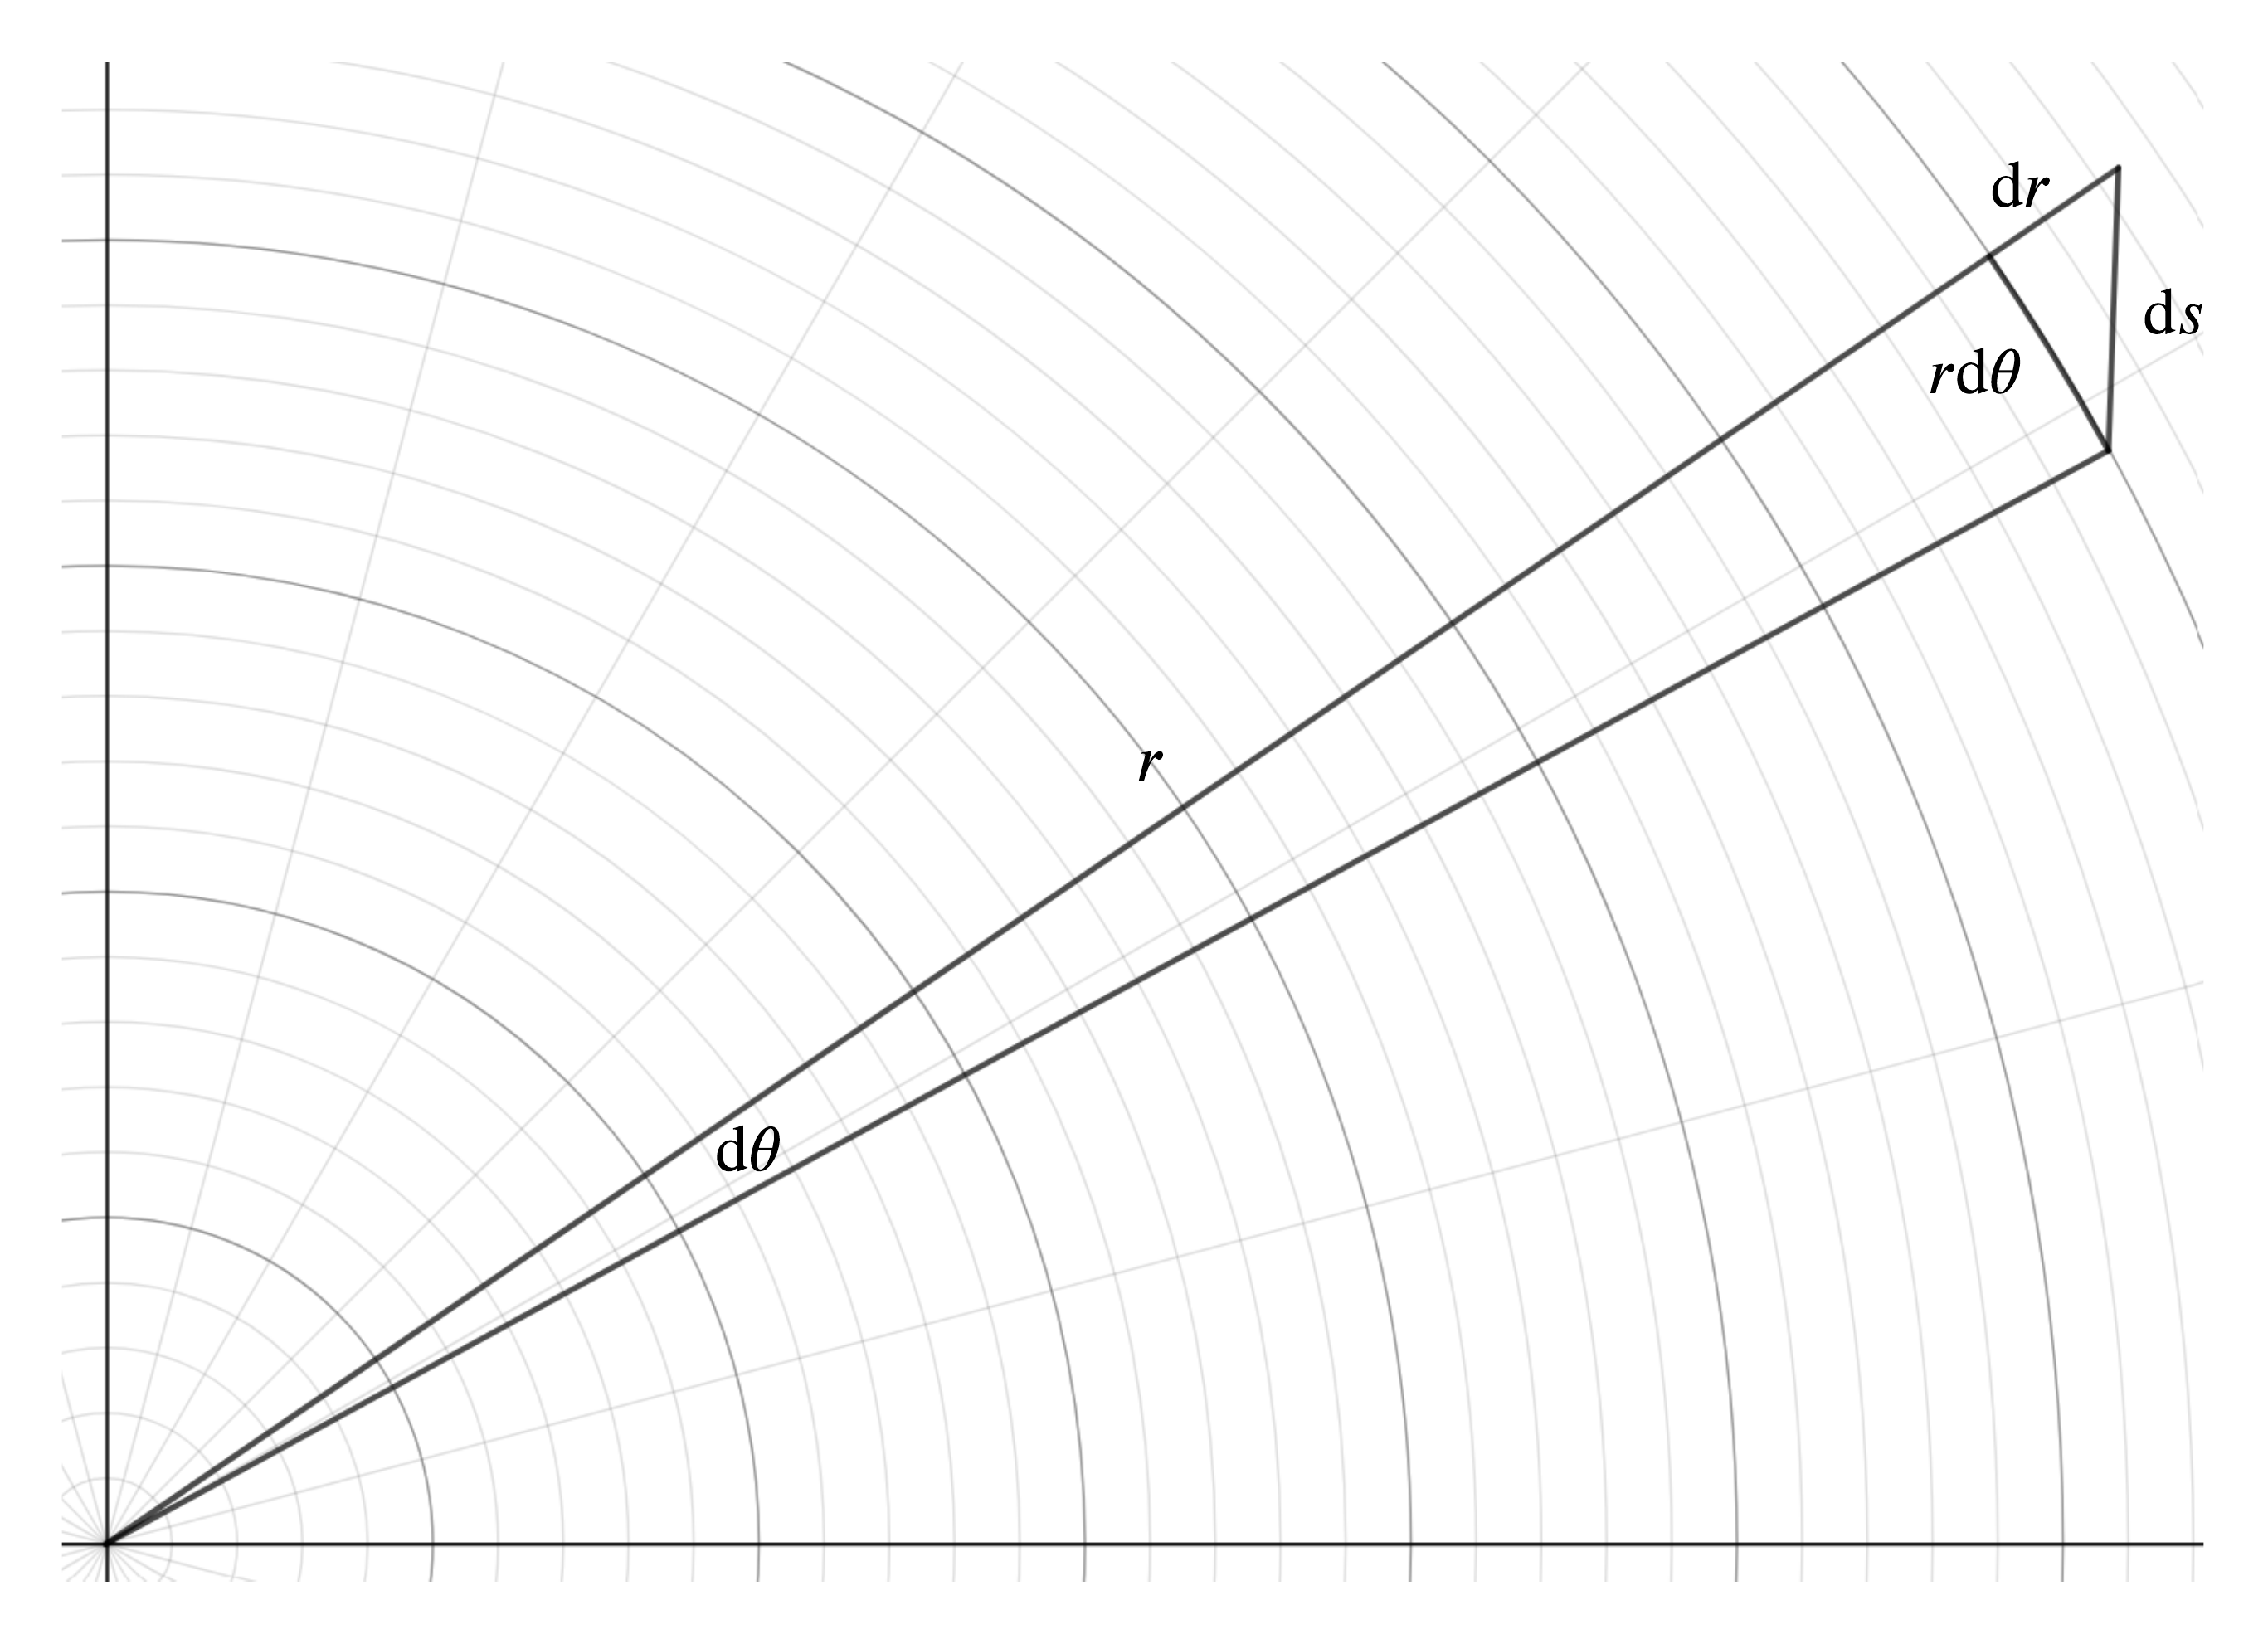
\includegraphics[width=0.66\textwidth]{./parametric_vector_polar/polar_length.png}
	\caption{\hyperref{}{}{}{Polar Arc Length}}
\end{figure}
We see that these changes for a right triangle with hypotenuse $\d{s}$.
\begin{align*}
	(\d{s})^2 &= (r\d{\theta})^2 + (\d{r})^2 \\
	&= \left(r^2 + \left(\dd{r}{\theta}\right)^2\right)\left(\d{\theta}\right)^2 \\
	\d{s} &= \sqrt{r^2 + \left(\dd{r}{\theta}\right)^2}\d{\theta} \\
	s &= \int_{\alpha}^{\beta}{\sqrt{r^2 + \left(\dd{r}{\theta}\right)^2}\d{\theta}}.
\end{align*}

Giving us an alternate formula for polar arc length.

\begin{example}
	Find the arc length of the cardioid $r=1-\cos{\theta}$.
\end{example}
\begin{answer}
	The bounds are $0 \leq \theta \leq 2\pi$.
	Using the polar arc length formula,
	\begin{align*}
		\dd{r}{\theta} &= \sin{\theta} \\
		\left(\dd{r}{\theta}\right)^2 &= \sin^2{\theta} \\
		s &= \int_{0}^{2\pi}{\sqrt{\left(1-\cos{\theta}\right)^2+\sin^2{\theta}}\d{\theta}} \\
		&= \int_{0}^{2\pi}{\sqrt{2+2\cos{\theta}}\d{\theta}} \\
		&= \int_{0}^{2\pi}{2\sin{\left(\frac{\theta}{2}\right)}\d{\theta}} \\
		&= -4\cos{\left(\frac{\theta}{2}\right)}\biggr\rvert_{0}^{2\pi} \\
		&= 8.
	\end{align*}
\end{answer}

		\chapter{Sequences, L'H\^{o}pital's Rule, \& Improper Integrals}

\section{Sequences}
\begin{definition}
	A sequence $\left\{a_n\right\} = \left\{a_1, a_2, \ldots, a_n\right\}$ is an ordered list of numbers.
	Each element of a sequences is called a term and is identified by its index in the sequence.
	Sequences can be finite or infinite.
\end{definition}

\begin{example}
	The nth term of a sequence is defined by the following formula:
	\begin{equation*}
		a_n = \frac{(-1)^n}{n^2+1}.
	\end{equation*}
	Find the 1st, 2nd, and 100th terms of the sequence.
\end{example}
\begin{align*}
	a_1 &= \frac{(-1)^1}{1^2 + 1} = \frac{-1}{2} \\
	a_2 &= \frac{(-1)^2}{2^2 + 1} = \frac{1}{5} \\
	a_{100} &= \frac{(-1)^{100}}{100^2 + 1} = \frac{1}{10001}.
\end{align*}

\noindent
The above sequence was defined explicitly, meaning that we have a formula for the nth term of the sequence only in terms of n.
However, sequences can also be defined recursively, meaning the formula for subsequent terms of the sequence contains previous terms.
For a recursive sequence to be properly defined, there need to be one or more base terms that aren't defined recursively.
For example, the Fibonacci sequence, one of the most famous recursive sequences, as $a_1$ and $a_2$ as base terms.
\begin{equation*}
	a_n = \begin{cases}
		1 & n = 1, 2 \\
		a_{n-1} + a_{n-2} & n \geq 3
	\end{cases}.
\end{equation*}

\subsection{Common Types of Sequences}
There are some common types of sequences that you should be familiar with.
You might recognize these types of sequences and some of the formulas surrounding them from previous math classes.

\subsubsection{Arithmetic Sequences}
\begin{definition}
	An arithmetic sequence is one where $a_{n+1} - a_{n} = d$, a common difference, for all terms.
\end{definition}
\noindent
That is, to get the next term, we simply add some number $d$ (which could be negative) to the previous term.
Arithmetic sequences can be defined either explicitly or recursively.
Let $a_0$ be the starting term of the sequence.
\begin{align*}
	a_n &= dn + a_0 \\
	&= \begin{cases}
		a_0 & n = 0 \\
		d + a_{n-1} & n \geq 1
	\end{cases}.
\end{align*}
As we can see from the explicit formula, if we graphed values of an arithmetic sequence on in the plane with $x$ coordinate $n$ and $y$ coordinate $a_n$, all points would lie on a line with slope $d$ and $y$ intercept $a_0$.

\begin{example}
	Write an explicit formula for the following arithmetic sequence.
	\begin{equation*}
		\left\{\ln{2}, \ln{6}, \ln{18}, \ldots\right\}.
	\end{equation*}
\end{example}
Since we are given that this sequence is arithmetic, we'll find the common difference.
\begin{equation*}
	d = \ln{6} - \ln{2} = \ln{\frac{6}{2}} = \ln{3}.
\end{equation*}
\indent
So, applying the explicit formula for an arithmetic sequence with starting term $\ln{2}$ and common difference $\ln{3}$,
\begin{equation*}
	a_n = \ln{(3)}n + \ln{2}, n\geq 0.
\end{equation*}
\indent
We might have also noticed that each term inside the $\ln$ is triple the previous one, meaning we can write an explicit formula and then simplify to the same answer as before.
\begin{align*}
	a_n &= \ln{(3^{n}\cdot 2)}, n\geq 0 \\
	&= \ln{3^n} + \ln{2}, n \geq 0 \\
	&= \ln{(3)}n + \ln{2}, n \geq 0.
\end{align*}

\subsubsection{Geometric Sequences}
\begin{definition}
	A geometric sequence is one where $\frac{a_{n+1}}{a_n} = r$, a common ratio, for all terms.
\end{definition}
\noindent
That is, to get the next term, we simply multiply some number $r$ (which could be negative) by the previous term.
Geometric sequences can also be defined explicitly or recursively.
Let $a_0$ be the starting term of the sequence.
\begin{align*}
	a_n &= a_0(r)^n \\
	&= \begin{cases}
		a_0 & n = 0 \\
		ra_{n-1} & n \geq 1
	\end{cases}.
\end{align*}
\noindent
As we can see with the explicit formula, if we graphed terms of a geometric sequence for positive $r$, the points would lie on an exponential curve with $y$ intercept $a_0$ and exponential base $r$.

\begin{example}
	Write an explicit formula for the following geometric sequence.
	\begin{equation*}
		\left\{2,-6,18,-54,\ldots\right\}.
	\end{equation*}
\end{example}
Since we are given that this sequence is geometric, we'll find the common ratio.
\begin{equation*}
	r = \frac{-6}{2} = 3.
\end{equation*}
\indent
So, applying the explicit formula for a geometric sequence with starting term 2 and common ratio -3,
\begin{equation*}
	a_n = 2(-3)^n.
\end{equation*}

\subsection{Limits of a Sequence}
Once we have a formula for a sequence, we might be interested to know if $a_n$ tends towards some value as $n$ gets large.
\begin{definition}
	Let $L$ be a real number, the sequence $\left\{a_n\right\}$ as limit $L$ as $n$ approaches infinity if given any real $\epsilon > 0$, there is some index $m$ such that for all $n > m$
	\begin{equation*}
		\abs{a_n - L} < \epsilon.
	\end{equation*}
	We notate this as 
	\begin{equation*}
		\lim_{n\to\infty}{a_n} = L
	\end{equation*}
	and say the sequence converges to $L$.
	If the sequence does not have a limit, then we say the sequences diverges.
\end{definition}

\noindent
The following rules we gave for limits of a function: Sum and Difference Rule, Product Rule, Constant Multiple Rule, and Quotient Rule, all still apply to limits of sequences.
The only rule that doesn't still hold is the Power Rule because of the following sort of problem:
\begin{align*}
	a_n &= (-1)^n \\
	\lim_{n\to\infty}{a_n^2} &= 1 \\
	\left(\lim_{n\to\infty}{a_n}\right)^2 &= \text{DNE} \\
	1 &\neq \text{DNE}.
\end{align*}

\subsubsection{The Sandwich Theorem for Sequences}
\begin{theorem}[Sandwich Theorem for Sequences]
	If $\lim_{n\to\infty}{a_n} = \lim_{n\to\infty}{c_n} = L$ and there is an integer $m$ such that $a_n \leq b_n \leq c_n$ for all $n > m$, then $\lim_{n\to\infty}{b_n} = L$.
\end{theorem}
\noindent
This is essentially the same as the Sandwich Theorem for limits of a function.
The only added caveat is that we have to find some index $m$ for which the sandwiching inequality always holds for terms after the $m$th.

\begin{example}
	Determine if the following sequence converges or diverges.
	If it converges, find its limit.
	\begin{equation*}
		a_n = (-1)^n\frac{n-1}{2}, n\geq 1.
	\end{equation*}
\end{example}
We see that as $n$ grows large $\abs{a_n}$ approaches 1.
However, $a_n$ bounces between 1 and -1 depending on whether $n$ is even or odd.
Thus, we could let $\epsilon = 1/2$, which would show that the limit diverges.

\begin{example}
	Determine if the following sequences converges or diverges.
	If it converges, find its limit.
	\begin{equation*}
		a_n = \frac{\cos{n}}{n}, n\geq 1.
	\end{equation*}
\end{example}
It might at first seem that this limit diverges because $\cos$ bounces between -1 and 1.
However, we can use the Sandwich Theorem to show that the limit converges.
\begin{align*}
	\frac{-1}{n} &\leq \frac{\cos{n}}{n} \leq \frac{1}{n}, n\geq 1 \\
	\lim_{n\to\infty}{\frac{-1}{n}} &\leq \lim_{n\to\infty}{\frac{\cos{n}}{n}} \leq \lim_{n\to\infty}{\frac{1}{n}} \\
	0 &\leq \lim_{n\to\infty}{\frac{\cos{n}}{n}} \leq 0 \\
	\lim_{n\to\infty}{\frac{\cos{n}}{n}} &= 0.
\end{align*}

\subsubsection{Absolute Value Theorem}
We can apply the Sandwich Theorem to show that sequences whose absolute value converges to 0 must also converge to 0.
\begin{theorem}[Absolute Value Theorem]
	If $\lim_{n\to\infty}{\abs{a_n}} = 0$, then $\lim_{n\to\infty}{a_n} = 0$.
\end{theorem}
\begin{proof}
	For all $n$,
	\begin{equation*}
		-\abs{a_n} \leq a_n \leq \abs{a_n}.
	\end{equation*}
	Applying the Sandwich Theorem and limit properties,
	\begin{align*}
		-\lim_{n\to\infty}{\abs{a_n}} &\leq \lim_{n\to\infty}{a_n} \leq \lim_{n\to\infty}{\abs{a_n}} \\
		-0 &\leq \lim_{n\to\infty}{a_n} \leq 0 \\
		\lim_{n\to\infty}{a_n} &= 0.
	\end{align*}
\end{proof}
\section{L'H\^{o}pital's Rule}
\subsection{Indeterminate Form 0/0}
If both $f(x)$ and $g(x)$ are 0 at $x=a$, then the limit
\begin{equation*}
	\lim_{x\to a}{\frac{f(x)}{g(x)}}
\end{equation*}
is an indeterminate form of 0/0, meaning we can't substitute $x=a$ to evaluate the limit.
However, L'\^{o}pital's Rule allows us to modify this limit to get another limit, which might not have this indeterminate form but is guaranteed to have the same limit.

\begin{theorem}[L'H\^{o}pital's Rule, Weaker Form]
	If $f(a) = g(a) = 0$; $f^\prime(a)$ and $g^\prime(a) \neq 0$ exist, then
	\begin{equation*}
		\lim_{x\to a}{\frac{f(x)}{g(x)}} = \frac{f^\prime(a)}{g^\prime(a)}.
	\end{equation*}
\end{theorem}
\begin{proof}
	\begin{align*}
		\lim_{x\to a}{\frac{f(x)}{g(x)}} &= \lim_{x\to a}{\frac{f(x)-0}{g(x)-0}} \\
		&= \lim_{x\to a}{\frac{f(x)-f(a)}{g(x)-g(a)}} \\
		&= \lim_{x\to a}{\frac{\frac{f(x)-f(a)}{x-a}}{\frac{g(x)-g(a)}{x-a}}} \\
		&= \frac{\lim_{x\to a}{\frac{f(x)-f(a)}{x-a}}}{\lim_{x\to a}{\frac{g(x)-g(a)}{x-a}}} \\
		&= \frac{f^\prime(a)}{g^\prime(a)}.
	\end{align*}
\end{proof}

\begin{example}
	Find $\lim_{x\to 2}{\frac{x^2-4}{x-2}}$ using L'H\^{o}pital's Rule.
\end{example}
\begin{answer}
	\begin{equation*}
		\lim_{x\to 2}{\frac{x^2-4}{x-2}} = \frac{2(2)}{1} = 4.
	\end{equation*}
	
	Note that we get the same answer if we didn't use L'H\^{o}pital's Rule and instead factored.
	\begin{equation*}
		\lim_{x\to 2}{\frac{x^2-4}{x-2}} = \lim_{x\to 2}{\frac{(x+2)(x-2)}{x-2}} \lim_{x\to 2}{x+2} = 4.
	\end{equation*}
\end{answer}


It's possible that $f^\prime(a) = g^\prime(a) = 0$, meaning we're still left with the indeterminate form 0/0.
However, we can use a stringer form of L'H\^{o}pital's Rule that allows us to not have to immediate substitute $x=a$ and allows us to apply the rule multiple times if needed.
\begin{theorem}[L'H\^{o}pital's Rule, Stronger Form]
	If $f(a)=g(a)=0$; $f$ and $g$ are differentiable on an open interval $I$ that contains $a$; $g^\prime(x)\neq 0$ if $x\neq a$, then
	\begin{equation*}
		\lim_{x\to a}{\frac{f(x)}{g(x)}} = \lim_{x\to a}{\frac{f^\prime(x)}{g^\prime(x)}}
	\end{equation*}
	if the right-hand limit exists.
\end{theorem}

\begin{example}
	Find the following limit or show that it doesn't exist.
	\begin{equation*}
		\lim_{x\to 0}{\frac{\cos{x}-1}{e^x - x - 1}}.
	\end{equation*}
\end{example}
\begin{answer}
	$\cos{0}-1 = 0 = e^0 - 0 - 1$; $e^x - x - 1 \neq 0$ if $x\neq 0$ on all real numbers.
	\begin{equation*}
		\lim_{x\to 0}{\frac{\cos{x}-1}{e^x - x - 1}} = \lim_{x\to 0}{\frac{-\sin{x}}{e^x - 1}}.
	\end{equation*}
	
	$-\sin{0} = 0 = e^0 - 1$; $e^x - 1 \neq 0$ if $x\neq 0$ on all real numbers.
	\begin{equation*}
		\lim_{x\to 0}{\frac{-\sin{x}}{e^x - 1}} = \lim_{x\to 0}{\frac{-\cos{x}}{e^x}} = \frac{-1}{1} = -1.
	\end{equation*}
\end{answer}

\subsection{Indeterminate Forms $\infty/\infty$, $\infty\cdot 0$, \& $\infty - \infty$}
\subsubsection{$\infty/\infty$}
L'H\^{o}pital's still applies as written for the indeterminate form $\infty/\infty$.

\begin{example}
	Find the following limit or show that it doesn't exist.
	\begin{equation*}
		\lim_{x\to\pi/2}\frac{\tan{x}}{1+\tan{x}}.
	\end{equation*}
\end{example}
\begin{answer}
	Applying L'H\^{o}pital's Rule,
	\begin{equation*}
		\lim_{x\to\pi/2}{\frac{\tan{x}}{1+\tan{x}}} = \lim_{x\to\pi/2}\frac{\sec^2{x}}{\sec^2{x}} = 1.
	\end{equation*}
\end{answer}

\subsubsection{$\infty\cdot 0$}
We need to rearrange the limit into a 0/0 or $\infty/\infty$ indeterminate form.
\begin{example}
	Find the following limit or show that it doesn't exist.
	\begin{equation*}
		\lim_{x\to\infty}{x\sin{\frac{1}{x}}}.
	\end{equation*}
\end{example}
\begin{answer}
	Rearranging,
	\begin{equation*}
		\lim_{x\to\infty}{x\sin{\frac{1}{x}}} = \lim_{x\to\infty}\frac{\sin{\frac{1}{x}}}{\frac{1}{x}}.
	\end{equation*}
	
	Since the limit now has indeterminate form 0/0, we can apply L'H\^{o}pital's Rule.
	\begin{equation*}
		\lim_{x\to\infty}\frac{\sin{\frac{1}{x}}}{\frac{1}{x}} = \lim_{x\to\infty}\frac{\frac{-1}{x^2}\cos{\frac{1}{x}}}{\frac{-1}{x^2}} = cos(0) = 1.
	\end{equation*}
\end{answer}

\subsubsection{$\infty - \infty$}
We need to rearrange the limit into a 0/0 or $\infty/\infty$ indeterminate form.
\begin{example}
	Find the following limit or show that it doesn't exist.
	\begin{equation*}
		\lim_{x\to 1}{\frac{1}{\ln{x}} - \frac{1}{x-1}}.
	\end{equation*}
\end{example}
\begin{answer}
	Rearranging,
	\begin{equation*}
		\lim_{x\to 1}{\frac{1}{\ln{x}} - \frac{1}{x-1}} = \lim_{x\to 1}{\frac{x-1-\ln{x}}{(x-1)\ln{x}}}.
	\end{equation*}
	Since the limit now has indeterminate form 0/0, we can apply L'H\^{o}pital's Rule.
	\begin{equation*}
		\lim_{x\to 1}{\frac{x-1-\ln{x}}{(x-1)\ln{x}}} = \lim_{x\to 1}{\frac{1-\frac{1}{x}}{(x-1)\frac{1}{x} + \ln{x}}} = \lim_{x\to 1}{\frac{\frac{1}{x^2}}{\frac{1}{x} - (x-1)\frac{1}{x^2} + \frac{1}{x}}} = \frac{1}{1-0+1} = \frac{1}{2}.
	\end{equation*}
\end{answer}

\subsection{Indeterminate Forms $1^\infty$, $0^0$, \& $\infty^0$}
For indeterminate forms with exponents, we should take the natural log of the limit, solve that limit, and then exponentiate.

\subsubsection{$1^\infty$}
\begin{example}
	Find the following limit or show that it doesn't exist.
	\begin{equation*}
		\lim_{x\to \infty}{\left(1+\frac{1}{x}\right)^x}.
	\end{equation*}
\end{example}
\begin{answer}
	Let $L$ be the value of the limit.
	\begin{align*}
		L &= \lim_{x\to \infty}{\left(1+\frac{1}{x}\right)^x} \\
		\ln{L} &= \lim_{x\to\infty}{\ln{\left(\left(1+\frac{1}{x}\right)^x\right)}} \\
		&= \lim_{x\to\infty}{x\ln{\left(1+\frac{1}{x}\right)}} \text{ (indeterminate form $\infty\cdot 0$)} \\
		&= \lim_{x\to\infty}{\frac{\ln{\left(1+\frac{1}{x}\right)}}{\frac{1}{x}}} \text{ (indeterminate form $0/0$)} \\
		&= \lim_{x\to\infty}{\frac{\frac{1}{1+\frac{1}{x}}\frac{-1}{x^2}}{\frac{-1}{x^2}}} \\
		&= \lim_{x\to\infty}{\frac{1}{1+\frac{1}{x}}} \\
		&= 1 \\
		e^{\ln{L}} &= e^1 \\
		L &= e.
	\end{align*}
\end{answer}

\subsubsection{$0^0$}
\begin{example}
	Find the following limit or show that it doesn't exist.
	\begin{equation*}
		\lim_{x\to 0^+}{x^x}.
	\end{equation*}
\end{example}
\begin{answer}
	Let $L$ be the value of the limit.
	\begin{align*}
		L &= \lim_{x\to 0^+}{x^x} \\
		\ln{L} &= \lim_{x\to 0^+}{x\ln{x}} \text{ (indeterminate form $0\cdot-\infty$)} \\
		&= \lim_{x\to 0^+}{\frac{\ln{x}}{\frac{1}{x}}} \text{ (indeterminate form $-\infty/\infty$)} \\
		&= \lim_{x\to 0^+}{\frac{\frac{1}{x}}{\frac{-1}{x^2}}} \\
		&= \lim_{x\to 0^+}{\frac{1}{\frac{-1}{x}}} \\
		&= \lim_{x\to 0^+}{-x} \\
		&= 0 \\
		e^{\ln{L}} &= e^0 \\
		L &= 1.
	\end{align*}
\end{answer}

\subsubsection{$\infty^0$}
\begin{example}
	Find the following limit or show that it doesn't exist.
	\begin{equation*}
		\lim_{x\to\infty}{x^{\frac{1}{x}}}.
	\end{equation*}
\end{example}
\begin{answer}
	Let $L$ be the value of the limit.
	\begin{align*}
		L &= \lim_{x\to\infty}{x^{\frac{1}{x}}} \\
		\ln{L} &= \lim_{x\to\infty}{\frac{1}{x}\ln{x}} \text{ (indeterminate form $0\cdot\infty$)} \\
		&= \lim_{x\to\infty}{\frac{\ln{x}}{x}} \text{ (indeterminate form $\infty/\infty$)} \\
		&= \lim_{x\to\infty}{\frac{\frac{1}{x}}{1}} \\
		&= 0 \\
		e^{\ln{L}} &= e^0 \\
		L &= 1.
	\end{align*}
\end{answer}
\section{Relative Growth Rates}
In many practical applications, like the run times of computer algorithms for example, we often want to know if a function grows slower, the same, or faster than another.
\begin{definition}
	If
	\begin{equation*}
		\lim_{x \to \infty}{\frac{f(x)}{g(x)}} = \infty \Leftrightarrow \lim_{x \to \infty}{\frac{g(x)}{f(x)}} = 0,
	\end{equation*}
	then $f$  grows faster than $g$.
	If
	\begin{equation*}
		\lim_{x \to \infty}{\frac{f(x)}{g(x)}} = c \Leftrightarrow \lim_{x \to \infty}{\frac{g(x)}{f(x)}} = \frac{1}{c}
	\end{equation*}
	for some non-zero constant $c$, then $f$ and $g$ grow at the same rate.
\end{definition}

\begin{example}
	Compare $e^x$ and $x^{100}$.
	Does one grow faster than the other, or do they grow at the same rate?
\end{example}
\begin{answer}
	\begin{align*}
		\lim_{x\to\infty}{\frac{e^x}{x^{100}}} &= \lim_{x\to\infty}{\frac{e^x}{100x^{99}}} \\
		&= \vdots \text{ (after many applications of L'H\^{o}pital's Rule)} \\
		&= \lim_{x\to\infty}{\frac{e^x}{100!}}
		&= \infty.
	\end{align*}
	
	So, $e^x$ grows faster than $x^{100}$.
	In fact, any exponential $b^x$ grows faster than any polynomial, as long as $b > 1$.
\end{answer}

\subsection{Transitive Grow Rates}
For sufficiently large $x$, growth rates are transitive.
That is, if $f$ grows the same/faster/slower/ than $g$, and $g$ grows the same/slower/faster than $h$, then $f$ also grows the same/faster/slower than $h$.

\begin{example}
	Show that $f(x)=\sqrt{x^2+5}$ and $g(x)=\left(2\sqrt{x}-1\right)^2$ grow at the same rate.
\end{example}
\begin{answer}
	We'll show that both $f$ and $g$ grow at the same rate as $h(x)=x$.
	Starting with $f$ and $h$,
	\begin{align*}
		\lim_{x\to\infty}{\frac{f(x)}{h(x)}} &= \lim_{x\to\infty}{\frac{\sqrt{x^2+5}}{x}} \\
		&= \lim_{x\to\infty}{\sqrt{\frac{x^2+5}{x^2}}} \\
		&= \sqrt{\lim_{x\to\infty}{\frac{x^2+5}{x^2}}} \text{ (by the Power Rule)} \\
		&= \sqrt{1} \\
		&= 1.
	\end{align*}
	
	So, $f$ and $h$ grow at the same rate.
	Moving on to $g$ and $h$,
	\begin{align*}
		\lim_{x\to\infty}{\frac{g(x)}{h(x)}} &= \lim_{x\to\infty}{\frac{\left(2\sqrt{x}-1\right)^2}{x}} \\
		&= \lim_{x\to\infty}{\left(\frac{2\sqrt{x}-1}{\sqrt{x}}\right)^2} \\
		&= \left(\lim_{x\to\infty}{\frac{2\sqrt{x}-1}{\sqrt{x}}}\right)^2 \text{ (by the Power Rule)} \\
		&= \left(2\right)^2 \\
		&= 4.
	\end{align*}
	
	So, $g$ and $h$ grow at the same rate.
	Since $f$ and $g$ both grow at the same rate as $h$, $f$ and $g$ must grow at the same rate as each other.
\end{answer}

\subsection{Growth Rate Hierarchy ($n^n$FEPL)}
For most of the common types of functions we see, we can establish families of functions and rank these families by their growth rates from fastest-growing to slowest-growing.
If two functions are in different families, we can be sure that one grows faster than the other.
If two functions are in the same family, we'll have to do more work to compare them.
These families are summarized by the acronym $n^n$FEPL\footnote{You might recognize these families as a sort of Big-O family from computer science.}.
\begin{itemize}[align=left, leftmargin=0.66in]
	\item[$\textbf{n}^\textbf{n}$] These are functions that have a variable both in the base and exponent.
	\item[\textbf{F}actorials] These are functions that have an $n!$ term.
	\item[\textbf{E}xponentials] These are functions that have a constant base and a variable exponent.
		Note that if the variable base if less than 1, the function actually gets smaller for larger $n$.
	\item[\textbf{P}olynomials] These are functions with a variable base and constant exponent.
		Certain polynomials can still grow faster than others.
		For example, $x^2$ grows faster than $x$, which grows faster than $\sqrt{x}$.
	\item[\textbf{L}ogarithms] These are functions that have a log of a polynomial.
\end{itemize}

Although these rules are indeed true, don't just apply them blindly.
You should try to simplify a function first before figuring out to which family it belongs.
For example, although $\ln{x^x}$ contains an $x^x$ and a $\ln$, it's neither in the $n^n$ family nor in the logarithms family.
In fact, although this function is not a polynomial, it grows faster than $x$ but slower than $x^2$. \\


A function belongs to the family of its fastest-growing positive term.
Negative terms can either be ignored or used to simplify other terms.
For example, although $x^3 + e^x$ contains a polynomial $x^3$ term, for very large $x$, the $e^x$ term dominates the growth, meaning this function is part of the exponentials family.
\section{Improper Integrals}
Now that we've developed the tools to deal with limits as they approach infinity and the possible indeterminate forms that may arise, we can apply these ideas to integrals, allowing us to have $-\infty$ and $\infty$ as limits of integration.
We call these integrals with $\pm\infty$ as limits of integration, and functions that become $\pm\infty$ somewhere within the interval we're integrating on improper integrals.

\subsection{Infinite Integration Limits}
\begin{definition}
	If $f$ is continuous on $[a,\infty)$, then
	\begin{equation*}
		\int_{a}^{\infty}{f(x)\d{x}} = \lim_{b\to\infty}{\int_{a}^{b}{f(x)\d{x}}}.
	\end{equation*}
	If $f$ is continuous on $(-\infty,b]$, then
	\begin{equation*}
		\int_{\infty}^{b}{f(x)\d{x}} = \lim_{a\to-\infty}{\int_{a}^{b}{f(x)\d{x}}}.
	\end{equation*}
	If $f$ is continuous on $(-\infty,\infty)$, then
	\begin{equation*}
		\int_{-\infty}^{\infty}{f(x)\d{x}} = \int_{-\infty}^{c}{f(x)\d{x}} + \int_{c}^{\infty}{f(x)\d{x}}
	\end{equation*}
	for any real constant $c$.
	If these limits exist, then the integral converges and has a value.
	Otherwise, the integral diverges and does not have a value.
\end{definition}

\begin{example}
	Evaluate the following integral or state that it diverges.
	\begin{equation*}
		\int_{2}^{\infty}{\frac{3}{x^2-x}\d{x}}.
	\end{equation*}
\end{example}
\begin{answer}
	Applying the definition,
	\begin{align*}
		\int_{2}^{\infty}{\frac{3}{x^2-x}\d{x}} &= \lim_{b\to\infty}{\int_{2}^{b}{\frac{3}{x^2-x}\d{x}}} \\
		&= \lim_{b\to\infty}{3\int_{2}^{b}{\left(\frac{1}{x-1}-\frac{1}{x}\right)\d{x}}} \\
		&= \lim_{b\to\infty}{3\ln{\bigg\lvert\frac{x-1}{x}\bigg\rvert}\Biggr\rvert_{2}^{b}} \\
		&= \lim_{b\to\infty}{3\ln{\bigg\lvert\frac{b-1}{b}\bigg\rvert}} - 3\ln{\bigg\lvert\frac{1}{2}\bigg\rvert} \\
		&= 0 + 3\ln{2} \\
		&= 3\ln{2}.
	\end{align*}
\end{answer}

\begin{example}
	Evaluate the following integral or state that it diverges.
	\begin{equation*}
		\int_{1}^{\infty}{\frac{\d{x}}{\sqrt[4]{x}}}.
	\end{equation*}
\end{example}
\begin{answer}
	Applying the definition,
	\begin{align*}
		\int_{1}^{\infty}{\frac{\d{x}}{\sqrt[4]{x}}} &= \lim_{b\to\infty}{\int_{1}^{b}{\frac{\d{x}}{\sqrt[4]{x}}}} \\
		&= \lim_{b\to\infty}{\frac{4}{3}\sqrt[4]{x^3}\biggr\rvert_{1}^{b}} \\
		&= \lim_{b\to\infty}{\frac{4}{3}\sqrt[4]{b^3}} - \frac{4}{3}\sqrt[4]{1^3} \\
		&= \infty - \frac{4}{3} \\
		&= \text{diverges}.
	\end{align*}
\end{answer}

\subsection{Infinite Discontinuities}
An infinite discontinuity occurs when a function takes on a value of $\pm\infty$ on the interval we're integrating on.
In this case, we'll need to split the integral into pieces, evaluating the limit as we approach this infinite discontinuity from both sides.
\begin{definition}
	If $f$ is continuous on $(a,b]$, then
	\begin{equation*}
		\int_{a}^{b}{f(x)\d{x}} = \lim_{c\to a^+}{\int_{c}^{b}{f(x)\d{x}}}.
	\end{equation*}
	If $f$ is continuous on $[a,b)$, then
	\begin{equation*}
		\int_{a}^{b}{f(x)\d{x}} = \lim_{c\to b^-}{\int_{a}^{c}{f(x)\d{x}}}.
	\end{equation*}
	If $f$ is continuous on $[a,c) \cup (c,b]$, then
	\begin{equation*}
		\int_{a}^{b}{f(x)\d{x}} = \int_{a}^{c}{f(x)\d{x}} + \int_{c}^{b}{f(x)\d{x}}.
	\end{equation*}
	If these limits exist, then the integral converges and has a value.
	Otherwise, the integral diverges and does not have a value.
\end{definition}

\begin{example}
	Evaluate the following integral or state that it diverges.
	\begin{equation*}
		\int_{0}^{1}{\frac{\d{x}}{x^2}}.
	\end{equation*}
\end{example}
\begin{answer}
	We see that we have an infinite discontinuity at $x=0$.
	Applying the definition,
	\begin{align*}
		\int_{0}^{1}{\frac{\d{x}}{x^2}} &= \lim_{c\to 0^+}{\int_{c}^{1}{\frac{\d{x}}{x^2}}} \\
		&= \lim_{c\to 0^+}{\frac{-1}{x}\biggr\rvert_{c}^{1}} \\
		&= \frac{-1}{1} + \lim_{c\to 0^+}{\frac{1}{c}} \\
		&= -1 + \infty \\
		&= \text{diverges}.
	\end{align*}
\end{answer}

\begin{example}
	Evaluate the following integral or state that it diverges.
	\begin{equation*}
		\int_{0}^{1}{\frac{\d{x}}{x^{1/2}}}.
	\end{equation*}
\end{example}
\begin{answer}
	We see that we have an infinite discontinuity at $x=0$.
	Applying the definition,
	\begin{align*}
		\int_{0}^{1}{\frac{\d{x}}{x^{1/2}}} &= \lim_{c\to 0^+}{\int_{c}^{1}{\frac{\d{x}}{x^{1/2}}}} \\
		&= \lim_{c\to 0^+}{2x^{1/2}\biggr\rvert_{c}^{1}} \\
		&= 2 - \lim_{c\to 0^+}{2c^{1/2}} \\
		&= 2 - 0 \\
		&= 2.
	\end{align*}
\end{answer}

\subsection{Convergence Tests}
\subsubsection{P-Test}
\begin{lemma}
	The following integral will converge when $p > 1$ and diverge if $0 < p \leq 1$.
	\begin{equation*}
		\int_{1}^{\infty}{\frac{\d{x}}{x^p}}.
	\end{equation*}
\end{lemma}

\begin{example}
	Evaluate the following integral or state that it diverges.
	\begin{equation*}
		\int_{1}^{\infty}{\frac{\d{x}}{x}}.
	\end{equation*}
\end{example}
\begin{answer}
	We have an integral where $p=1$.
	So, by the P-Test, the integral diverges.
\end{answer}

\begin{example}
	Evaluate the following integral or state that it diverges.
	\begin{equation*}
		\int_{1}^{\infty}{\frac{\d{x}}{x^{1.001}}}.
	\end{equation*}
\end{example}
\begin{answer}
	We have an integral where $p=1.001$.
	So, by the P-Test, the integral converges.
	\begin{align*}
		\int_{1}^{\infty}{\frac{\d{x}}{x^{1.001}}} &= \lim_{b\to\infty}{\int_{1}^{b}{\frac{\d{x}}{x^{1.001}}}} \\
		&= \lim_{b\to\infty}{-1000x^{-0.001}\biggr\rvert_{1}^{b}} \\
		&= \lim_{b\to\infty}{-1000b^{-0.001}} + 1000(1)^{-0.001} \\
		&= 0 + 1000 \\
		&= 1000.
	\end{align*}
\end{answer}

\subsubsection{Direct Comparison Test}
\begin{lemma}
	Let $f$ and $g$ be continuous on $[a,\infty)$ with $0 \leq f(x) \leq g(x)$ for all $x \geq a$.
	\begin{align*}
		\int_{a}^{\infty}{f(x)\d{x}} &\text{ converges if } \int_{a}^{\infty}{g(x)\d{x}} \text{ converges.} \\
		\int_{a}^{\infty}{g(x)\d{x}} &\text{ diverges if } \int_{a}^{\infty}{f(x)\d{x}} \text{ diverges.}
	\end{align*}
\end{lemma}

That is, if a larger function converges, then so will a smaller funtion; if a smaller function diverges, then so will a larger function. \\


The hardest part of the Direct Comparison Test is deciding what function you should compare to.
A general rule is to pick a function that is similar to, but simpler than then given function.

\begin{example}
	Evaluate the following integral or state that it diverges.
	\begin{equation*}
		\int_{1}^{\infty}{\frac{\d{x}}{x^2-0.1}}.
	\end{equation*}
\end{example}
\begin{answer}
	If the 0.1 wasn't inside the square root, the function would simplify to $1/x$.
	Since the 0.1 is subtracted, the denominator is smaller than $1/x$.
	So, $1/x$ is a function that is smaller on $[1,\infty)$, meaning if it diverges, then so will the original function.
	We know by the P-Test that the integral of $1/x$ from 1 to $\infty$ will diverge, so the original function also diverges.
\end{answer}

\begin{example}
	Evaluate the following integral or state that it diverges.
	\begin{equation*}
		\int_{1}^{\infty}{e^{-x^2}\d{x}}.
	\end{equation*}
\end{example}
\begin{answer}
	Since the exponent is negative, a smaller exponent would mean a larger value.
	So, $e^{-x}$ is a larger function on $[1,\infty)$.
	\begin{equation*}
		\int_{1}^{\infty}{e^{-x}\d{x}} = \frac{1}{e},
	\end{equation*}
	meaning it converges, so the original function also converges.
\end{answer}

\subsubsection{Limit Comparison Test}
\begin{lemma}
	If positive functions $f$ and $g$ are continuous on $[a,\infty)$ and
	\begin{equation*}
		\lim_{x\to\infty}{\frac{f(x)}{g(x)}}
	\end{equation*}
	converges to a positive real number, then
	\begin{equation*}
		\int_{a}^{\infty}{f(x)\d{x}} \text { and } \int_{a}^{\infty}{g(x)\d{x}}
	\end{equation*}
	both converge or both diverge.
\end{lemma}


Many functions to which you can apply the Limit Comparison Test you can also apply the Direct Comparison Test.
The practical use of the limit comparison test is to take an uglier function, that may be tedious to integrate and compare it to a function that is easy to determine whether it diverges using something like the P-Test.
A common strategy, especially for rational functions, is to look at their end behavior model.

\begin{example}
	Evaluate the following integral or state that it diverges.
	\begin{equation*}
		\int_{1}^{\infty}{\frac{\d{x}}{1+x^2}}.
	\end{equation*}
\end{example}
\begin{answer}
	Although you might recognize this as the derivative of $\arctan$, let's continue with the Direct Comparison Test.
	This function looks very similar to $1/x^2$, which we know by the P-Test will converge on $[1,\infty)$.
	\begin{equation*}
		\lim_{x\to\infty}{\frac{\frac{1}{x^2}}{\frac{1}{1+x^2}}} = \lim_{x\to\infty}{\frac{1+x^2}{x^2}} = 1.
	\end{equation*}
	Since 1 is a positive real constant and the integral of $1/x^2$ converges, then the original integral also converges by the Limit Comparison Test.
\end{answer}

\begin{example}
	Evaluate the following integral or state that it diverges.
	\begin{equation*}
		\int_{1}^{\infty}{\frac{3x+6}{1-5x+7x^2}\d{x}}.
	\end{equation*}
\end{example}
\begin{answer}
	Looking at this rational function, we see a degree 1 polynomial in the numerator and a degree 2 polynomial in the denominator.
	So, we'd expect this rational function to have the same end behavior model as $1/x$, which we know by the P-Test diverges.
	\begin{equation*}
		\lim_{x\to\infty}{\frac{\frac{3x+6}{1-5x+7x^2}}{\frac{1}{x}}} = \lim_{x\to\infty}{\frac{3x^2+6x}{7x^2-5x+1}} = \frac{3}{7}.
	\end{equation*}
	Since 3/7 is a positive real constant and the integral of $1/x$ diverges, the the original integral also diverges by the Limit Comparison Test.
\end{answer}
		\chapter{Infinite Series}
We previously discussed some special types of series and formulas for their nth term.
Now, we'll look at sums of infinitely many terms and eventually see how summing variables rather than just numbers allows us to approximate functions.

\section{Power Series}
\subsection{Geometric Series}
First, we need to define what we mean by an infinite series.
\begin{definition}
	An infinite series is of the form
	\begin{equation*}
		a_1 + a_2 + \ldots + a_n + \ldots \text{ or equivalently, } \sum_{k=1}^{\infty}{a_k}.
	\end{equation*}
	Just like with finite series, each $a_i$ is a term, and $a_n$ is the nth term.
\end{definition}

We can describe the behavior of an infinite series by looking at how its value behaves after summing a finite number of terms.
We can define what it means for an infinite sum to have a value by looking at the limit of the partial sums as $n$ grows large.
\begin{definition}
	The nth partial sum of an infinite series is
	\begin{equation*}
		s_n = \sum_{k=1}^{n}{a_k}.
	\end{equation*}
	The infinite series converges to value $L$ if
	\begin{equation*}
		\lim_{n\to\infty}{s_n} = L.
	\end{equation*}
	Otherwise, the series diverges and does not have a value.
\end{definition}

\begin{example}
	State if the following infinite series converges or diverges.
	\begin{equation*}
		\frac{3}{10} + \frac{3}{100} + \ldots + \frac{3}{10^n} + \ldots.
	\end{equation*}
\end{example}
\begin{answer}
	Looking at the partial sums,
	\begin{align*}
		s_1 &= 0.3 \\
		s_2 &= 0.33 \\
		&\vdots \\
		s_n &= 0.\underbrace{33333\ldots}_{\text{$n$ total 3's}}
	\end{align*}
	
	So, it seems the limit of the partial sums tends towards a decimal with an infinite number of 3's.
	This value corresponds to the decimal expansion of 1/3, which clearly is real and finite, so the series converges.
\end{answer}


The above series is a geometric series since each subsequent term is 10 times smaller than the previous one (i.e $r=1/10$).
\begin{lemma}
	The geometric series
	\begin{equation*}
		\sum_{k=0}^{\infty}{a_0(r)^k}
	\end{equation*}
	converges to a value of $a_0/(1-r)$ if $\abs{r} < 1$ and diverges otherwise.
\end{lemma}
\begin{proof}
	We'll first find a formula for the partial sums and then find the limit of the partial sums for $1 < r < 1$.
	\begin{align*}
		s_n &= \sum_{k=0}^{n}{a_0(r)^k} \\
		&= a_0 + a_0r + a_0r^2 + \ldots + a_0r^n \\
		rs_n &= a_0r + a_0r^2 + a_0r^3 + \ldots + a_0r^n + a_0r^{n+1} \\
		&= -a_0 + s_n + a_0r^{n+1} \\
		s_n(r-1) &= a_0\left(r^{n+1} - 1\right) \\
		s_n &= a_0\frac{r^{n+1}-1}{r-1}.
	\end{align*}
	This formula for partial sums holds for all values of $r$.
	Now we'll take the limit of $s_n$ and see for what values of $r$ the limit exists.
	\begin{align*}
		\sum_{k=0}^{\infty}{a_0(r)^n} &= \lim_{n\to\infty}{s_n} \\
		&= \lim_{n\to\infty}{a_0\frac{r^{n+1}-1}{r-1}} \\
		&= \frac{-a_0}{r-1}, \abs{r} < 1 \\
		&= \frac{a_0}{1-r}, \abs{r} < 1.
	\end{align*}
\end{proof}

\subsection{Functions from Geometric Series}
What happens if rather than letting $r$ be some fixed value we know beforehand, we let $r$ be some variable $x$?
Applying the formula,
\begin{equation*}
	a_0 + a_0x + a_0x^2 + \ldots = \frac{a_0}{1-x}, \abs{x} < 1.
\end{equation*}
This sort of sum of powers of $x$ is called a power series, and the condition that $\abs{x}<1$ is called the interval of convergence.
Right now, this power series is centered at $x=0$, but we can generalize it a bit to be centered at $x=h$.
\begin{equation*}
	a_0 + a_0(x-h) + a_0(x-h)^2 + \ldots = \frac{a_0}{1-(x-h)}, \abs{x-h} < 1.
\end{equation*}
Note that this formula allows us to find the power series of any function $a_0/(mx+b)$.
\begin{equation*}
	\frac{a_0}{mx + b} = \frac{a_0}{1-(1-mx-b)} = a_0 + a_0(1-mx+b) + a_0(1-mx+b)^2 + \ldots, \abs{1-mx-b} < 1.
\end{equation*}
So,
\begin{align*}
	\frac{1}{x} &= 1 + (1-x) + (1-x)^2 + \ldots, \abs{1-x} < 1 \\
	\frac{1}{1-x} &= 1 + x + x^2 + x^3 + \ldots, \abs{x} < 1 \\
	\frac{1}{1+x} &= 1 - x + x^2 - x^3 + \ldots, \abs{x} < 1.
\end{align*}

\subsubsection{Term-By-Term Differentiation}
\begin{theorem}
	If the power series
	\begin{equation*}
		f(x) = \sum_{k=0}^{\infty}{c_k(x-a)^k} = c_0 + c_1(x-a) + c_2(x-a)^2 + \ldots
	\end{equation*}
	converges for $\abs{x-a} < R$, including $R=\infty$, then the power series
	\begin{equation*}
		\sum_{k=1}^{\infty}{kc_k(x-a)^{k-1}} = c_1 + 2c_2(x-a) + 3c_3(x-a)^2 + \ldots
	\end{equation*}
	also converges for $\abs{x-a} < R$ and is equal to $f^\prime(x)$ on that interval.
\end{theorem}

Applying the theorem,
\begin{align*}
	\frac{-1}{x^2} &= -1 - 2(1-x) - 3(1-x)^2 - \ldots, \abs{1-x} < 1 \\
	\frac{1}{(1-x)^2} &= 1 + 2x + 3x^2 + \ldots, \abs{x} < 1 \\
	\frac{-1}{(1+x)^2} &= -1 + 2x - 3x^2 + \ldots, \abs{x} < 1.
\end{align*}

\subsubsection{Term-By-Term Integration}
\begin{theorem}
	If the power series
	\begin{equation*}
		f(x) = \sum_{k=0}^{\infty}{c_k(x-a)^k} = c_0 + c_1(x-a) + c_2(x-a)^2 + \ldots
	\end{equation*}
	converges for $\abs{x-a} < R$, including $R=\infty$, then the power series
	\begin{equation*}
		\sum_{k=0}^{\infty}{c_k\frac{(x-a)^{k+1}}{k+1}} = c_0(x-a) + c_1\frac{(x-a)^2}{2} + c_2\frac{(x-a)^3}{3} + \ldots
	\end{equation*}
	also converges for $\abs{x-a} < R$ and represents the antiderivative of $f$ on that interval.
\end{theorem}

Applying the theorem,
\begin{align*}
	\ln{\abs{x}} &= 1 + \frac{(1-x)^2}{2} + \frac{(1-x)^3}{3} + \ldots, \abs{1-x} < 1 \\
	-\ln{\abs{1-x}} &= x + \frac{x^2}{2} + \frac{x^3}{3} + \ldots, \abs{x} < 1 \\
	\ln{\abs{1+x}} &= x - \frac{x^2}{2} + \frac{x^3}{3} - \frac{x^4}{4} + \ldots, \abs{x} < 1.
\end{align*}

This is pretty impressive: we now have an formula for $\ln{x}$ in terms of polynomials.
This also includes some pretty surprising identities.
For example\footnote{Technically, we're substituting $x=1$ which isn't in the interval of convergence. However, since we are dealing with an alternating sum, the series will also converge for $x=-1$ and $x=1$.},
\begin{equation*}
	\ln{2} = 1 - \frac{1}{2} + \frac{1}{3} - \ldots + \frac{(-1)^{n+1}}{n} + \ldots.
\end{equation*}

\begin{example}
	Find a power series for $\arctan{x}$ and state the interval of convergence.
\end{example}
\begin{answer}
	We know that
	\begin{equation*}
		\dd{}{x}\arctan{x} = \frac{1}{1+x^2}.
	\end{equation*}
	
	So, if we can find a power series that represents $1/(1+x^2)$, we can integrate term-by-term to get a power series for $\arctan{x}$.
	We also already know the following power series.
	\begin{equation*}
		\frac{1}{1+u} = 1 - u + u^2 - u^3 + \ldots, \abs{u} < 1.
	\end{equation*}
	
	Letting $u=x^2$,
	\begin{align*}
		\frac{1}{1+x^2} &= 1 - x^2 + x^4 - x^6 + \ldots, \abs{x^2} < 1 \\
		&= 1 - x^2 + x^4 - x^6 + \ldots, \abs{x} < 1.
	\end{align*}
	
	Integrating term-by-term,
	\begin{align*}
		\arctan{x} = x - \frac{x^3}{3} + \frac{x^5}{5} + \ldots + (-1)^n\frac{x^{2n+1}}{2n+1} + \ldots, \abs{x} < 1.
	\end{align*}
	
	This power series also gives rise to a pretty interesting identity\footnote{See footnote 1.}.
	\begin{equation*}
		\arctan{1} = \frac{\pi}{4} = 1 - \frac{1}{3} + \frac{1}{5} - \frac{1}{7} + \ldots + (-1)^n\frac{x^{2n+1}}{2n+1} \ldots.
	\end{equation*}
\end{answer}
\section{Taylor Series}
\subsection{Construction}
Although we can approximate lots of functions using power series derived from the geometric series, it'd be nice if we had a more general way to approximate any function using a power series.
We already have an approximation using a tangent line: the 0th and 1st derivatives of the function and line are equal at the point of tangency.
We could extend this idea of derivatives being equal to higher-order derivatives and higher degree polynomials.

\begin{example}
	Construct  polynomial $P(x)=a_0+a_1x + a_2x^2 + a_3x^3 + a_4x^4$ with the following behavior at $x=0$:
	\begin{align*}
		P(0) &= 1 \\
		P^\prime(0) &= 2 \\
		P^{\prime\prime}(0) &= 3 \\
		P^{\prime\prime\prime}(0) &= 4 \\
		P^{(4)}(0) &= 5.
	\end{align*}
\end{example}
Plugging in $x=0$ and solving for $a_0$,
\begin{align*}
	a_0 + a_1(0) + a_2(0)^2 + a_3(0)^4 + a_4(0)^4 &= 1 \\
	a_0 &= 1. 
\end{align*}
\indent
Differentiating once, plugging in $x=0$, and solvinf for $a_1$,
\begin{align*}
	P^\prime(x) &= a_1 + 2a_2x + 3a_3x^2 + 4a_4x^3 \\
	2 &= a_1 + 2a_2(0) + 3a_3(0)^2 + 4a_4(0)^3 \\
	a_1 &= 2.
\end{align*}
\indent
Continuing with differentiating and plugging in $x=0$, we get $a_2 = \frac{3}{2}$, $a_3 = \frac{2}{3}$, and $a_4 = \frac{5}{25}$.
So,
\begin{equation*}
	P(x) = 1 + 2x + \frac{3}{2}x^2 + \frac{2}{3}x^3 + \frac{5}{24}x^4.
\end{equation*}

\begin{example}
	Construct a degree 4 polynomial that approximates $\ln{(1+x)}$ at $x=0$.
\end{example}
\begin{table}[H]
	\begin{center}
		\begin{tabular}{ccc}
			$f(x)$ & $P(x)$ & $a_n$ \\
			\hline
			$f(x)=\ln{(1+x)}$ & $P(x)=a_0 + a_1x + a_2x^2 + a_3x^3 + a_4x^4$ & \\
			$f(0)=\ln{(1+0)}=0$ & $P(0)=a_0$ & $a_0 = 0$ \\
			\hline
			$f^\prime(x)=\frac{1}{1+x}$ & $P^\prime(x) = a_1 + 2a_2x + 3a_3x^2 + 4a_4x^3$ & \\
			$f^\prime(0)=\frac{1}{1+0}=1$ & $P^\prime(0) = a_1$ & $a_1 = 1$ \\
			\hline
			$f^{\prime\prime}(x)=\frac{-1}{(1+x)^2}$ & $P^{\prime\prime}(x)=2a_2 + 6a_3x + 12a_4x^2$ & \\
			$f^{\prime\prime}(0)=\frac{-1}{(1+0)^2} = -1$ & $P^{\prime\prime}(x)=2a_2$ & $a_2 = \frac{-1}{2}$ \\
			\hline
			$f^{(3)}(x) = \frac{2}{(1+x)^3}$ & $P^{(3)}(x) = 6a_3 + 24a_4x$ & \\
			$f^{(3)}(0) = \frac{2}{(1+0)^3}=2$ & $P^{(3)}(0) = 6a_3$ & $a_3 = \frac{1}{3}$ \\
			\hline
			$f^{(4)}(x) = \frac{-6}{(1+x)^4}$ & $P^{(4)}(x) = 24a_4$ & \\
			$f^{(4)}(x) = \frac{-6}{(1+0)^4}=-6$ & $P^{(4)}(0) = 24a_4$ & $a_4 = \frac{-1}{4}$ \\
			\hline
		\end{tabular}
	\end{center}
\end{table}
\indent
So, our polynomial is
\begin{equation*}
	P(x) = x - \frac{x^2}{2} + \frac{x^3}{3} - \frac{x^4}{4}.
\end{equation*}
\indent
Note that this polynomial exactly matches the power series we derived for $\ln{(1+x)}$. \\
This polynomial is called the 4th order Taylor polynomial of $\ln{(1+x)}$ at $x=0$.
The series created from all order Taylor polynomials is called the Taylor series of $\ln{(1+x)}$ at $x=0$.

\subsection{Definition}
\begin{definition}
	Let $f$ be a $n$ times differentiable function where all derivatives exist at $x=a$.
	The Taylor series for $f$ at $x=a$ is
	\begin{equation*}
		\sum_{i=0}^{\infty}{\frac{f^{(i)}(x)}{i!}(x-a)^i} = f(a) + f^\prime(a)(x-a) + \frac{f^{\prime\prime}(a)}{2!}(x-a)^2 + \ldots + \frac{f^{(n)}(a)}{n!}(x-a)^n + \ldots.
	\end{equation*}
	The $n$th partial sum of the Taylor Series,
	\begin{equation*}
		P_n(x) = \sum_{i=0}^{n}{\frac{f^{(i)}(x)}{i!}(x-a)^i}
	\end{equation*}
	is the Taylor polynomial of order $n$ for $f$ at $x=a$.
\end{definition}
\noindent
When $a=0$ you might also hear Taylor series referred to as Maclaurin series.
Like power series, Taylor series have intervals of convergence.

\begin{example}
	Find the Taylor series for $e^x$ at $x=0$.
	Verify using term-by-term differentiation that $e^x$ is its own derivative.
\end{example}
We know that $e^x$ is its own derivative, so $f^{(i)}(0)=e^0 = 1$ for all $i$.
Applying the definition,
\begin{align*}
	e^x &= e^0 + e^0(x-0) + \frac{e^0}{2!}(x-0)^2 + \frac{e^0}{3!}(x-0)^3 + \ldots + \frac{e^0}{n!}(x-0)^n + \ldots \\
	&= 1 + x + \frac{x^2}{2!} + \frac{x^3}{3!} + \ldots + \frac{x^n}{n!} + \ldots.
\end{align*}
\indent
Differentiating term-by-term,
\begin{equation*}
	\dd{}{x}e^x = 1 + x + \frac{x^2}{2!} + \ldots + \frac{x^{n-1}}{(n-1)!} + \ldots
\end{equation*}
we see that we get the same series, confirming that $e^x$ is its own derivative.

\subsection{List of Common Maclaurin Series}
\begin{align*}
	\frac{1}{1-x} &= 1 + x + x^2 + \ldots = \sum_{i=0}^{\infty}{x^i}, \abs{x} < 1 \\
	\frac{1}{1+x} &= 1 - x + x^2 - \ldots = \sum_{i=0}^{\infty}{(-1)^ix^i}, \abs{x} < 1 \\
	e^x &= 1 + x + \frac{x^2}{2!} + \ldots = \sum_{i=0}^{\infty}{\frac{x^i}{i!}}, \text{ all real $x$} \\
	\sin{x} &= x - \frac{x^3}{3!} + \frac{x^5}{5!} - \ldots = \sum_{i=0}^{\infty}{(-1)^i\frac{x^{2i+1}}{(2i+1)!}}, \text{ all real $x$} \\
	\cos{x} &= 1 - \frac{x^2}{2!} + \frac{x^4}{4!} - \ldots = \sum_{i=0}^{\infty}{(-1)^i\frac{2^{2i}}{(2i)!}}, \text{ all real $x$} \\
	\ln{(1+x)} &= x - \frac{x^2}{2} + \frac{x^3}{3} - \ldots = \sum_{i=0}^{\infty}{(-1)^i\frac{x^{i+1}}{i+1}}, \abs{x} \leq 1 \\
	\arctan{x} &= x - \frac{x^3}{3} + \frac{x^5}{5} - \ldots = \sum_{i=0}^{\infty}{(-1)^i\frac{x^{2i+1}}{2i+1}}, \abs{x} \leq 1.
\end{align*}

\subsubsection{Euler's Identity}
You might have seen the identity $e^{i\pi} + 1 = 0$ or even $e^{ix} = \cos{x} + i\sin{x}$.
Using our common Taylor Series, we can derive this famous identity. \\

\noindent
Starting with the Taylor series for $e^{ix}$,
\begin{align*}
	e^{ix} &= 1 + (ix) + \frac{(ix)^2}{2!} + \frac{(ix)^3}{3!} + \frac{(ix)^4}{4!} + \frac{(ix)^5}{5!} + \ldots = \sum_{k=0}^{\infty}{\frac{(ix)^k}{k!}}, \text{ all real $x$} \\
	&= 1 + ix + i^2\frac{x^2}{2!} + i^3\frac{x^3}{3!} + i^4\frac{x^4}{4!} + i^5\frac{x^5}{5!} + \ldots = \sum_{k=0}^{\infty}{i^k\frac{x^k}{k!}}, \text{ all real $x$} \\
	&= 1 + ix - \frac{x^2}{2!} - i\frac{x^3}{3!} + \frac{x^4}{4!} + i\frac{x^5}{5!} - \ldots, \text{ all real $x$} \\
	&= \left(1 - \frac{x^2}{2!} + \frac{x^4}{4!} + \ldots \right) + i\left(x - \frac{x^3}{3!} + \frac{x^5}{5!} + \ldots \right) \\
	&= \cos{x} + i\sin{x}.
\end{align*}
\noindent
Plugging in $x=\pi$,
\begin{align*}
	e^{i\pi} &= \cos{\pi} + i\sin{\pi} \\
	&= -1 + 0 \\
	e^{i\pi} + 1 &= 0.
\end{align*}
\section{Approximation Error}
Although knowing these infinite Taylor series is nice, if we want to use them to find function values, we'll need to approximate.
This means only using some finite number of terms in the Taylor series for our approximation.
Because we're not using all the terms, we'll naturally have some truncation error.
We'd like to be able to say how big this truncation error is so we can be sure that our approximation is good enough.

\subsection{Alternating Series Estimation Theorem}
\begin{theorem}[Alternating Series Estimation Theorem]
	Let $s$ be a convergent, alternating (i.e the sign of each term alternates) series where the terms of $\abs{s}$ are strictly decreasing.
	Then the $n$th term truncation error is the same sign as and less than in absolute value the $(n+1)$th term.
\end{theorem}

\begin{example}
	Give a bound for the truncation error of using the first 10 terms of the Maclaurin series of $\ln{(1+x)}$ to approximate $\ln{2}$.
\end{example}
\begin{answer}
	The Maclaurin series for $\ln{(1+x)}$ is
	\begin{equation*}
		\ln{(1+x)} = x - \frac{x^2}{2} + \frac{x^3}{3} - \ldots = \sum_{k=0}^{\infty}{(-1)^k\frac{x^{k+1}}{k+1}}, \abs{x} \leq 1,
	\end{equation*}
	
	which is an alternating series.
	We see that to approximate $\ln{2}$, we'd use $x=1$, which is in the interval of convergence, so the series converges.
	The first missing term of the series is $1/11$.
	Let $s_{10}$ be the partial sum of the first 10 terms when $x=1$.
	By the Alternating Series Estimation Theorem,
	\begin{equation*}
		0 < \ln{2} - s_{10} < \frac{1}{11}.
	\end{equation*}
\end{answer}

\subsection{Taylor's Theorem}
Although the Alternating Series Estimation Theorem is useful for quickly bounding the error of alternating series, we'd like something that can apply more generally to all Taylor series.
\begin{theorem}[Taylor's Theorem]
	Let $f$ be a $k+1$ times differentiable function on an open interval $I$ containing $a$.
	Then for all $x$ in $I$,
	\begin{equation*}
		f(x) = f(a) + f^\prime(a)(x-a) + \frac{f^{\prime\prime}(a)}{2!}(x-a)^2 + \ldots + \frac{f^{(n)}(a)}{n!}(x-a)^n + R_n(x)
	\end{equation*}
	where
	\begin{equation*}
		\abs{R_n(x)} = \frac{\abs{f^{(n+1)}(c)}}{(n+1)!}\abs{x-a}^{n+1}
	\end{equation*}
	for some $c$ between $x$ and $a$.
\end{theorem}

We can use this theorem to find the maximum value of $\abs{R_n(x)}$ over some interval.
We can also be more precise about what it means for a Taylor series to converge to some function over some interval.
\begin{definition}
	Let $R_n(x)$ be the remainder of truncating after the degree $n$ term in the Taylor series for $f$ centered at $x=a$.
	If for all $x$ in some interval $I$ containing $a$,
	\begin{equation*}
		\lim_{n\to\infty}{R_n(x)} = 0,
	\end{equation*}
	then we say the Taylor series for $f$ at $x=a$ converges to $f$ on $I$.
\end{definition}

\begin{example}
	Show that the Maclaurin series for $\sin{x}$ converges to $\sin{x}$ for all real $x$.
\end{example}
\begin{answer}
	We need to find the remainder and show that in the limit it goes to 0 as $n$ grows large.
	By Taylor's Theorem,
	\begin{align*}
		\abs{R_n(x)} &= \frac{\abs{f^{(n+1)}(c)}}{(n+1)!}\abs{x-a}^{n+1} \\
		&\leq \frac{\abs{x}^{n+1}}{(n+1)!}.
	\end{align*}
	
	The numerator is an exponential function, while the denominator is a factorial function, so using $n^n$FEPL,
	\begin{align*}
		0 \leq \lim_{n\to\infty}{R_n(x)} &\leq \lim_{n\to\infty}{\frac{\abs{x}^{n+1}}{(n+1)!}} = 0. \\
		\lim_{n\to\infty}{R_n(x)} &= 0.
	\end{align*}
	
	So, the Maclaurin series converges to $\sin{x}$ for all real $x$.
\end{answer}

\subsubsection{Remainder Estimation Theorem}
Notice that we didn't have to actually find the value of $f^{(n+1)}(c)$.
We just had to find a suitable upper bound where the limit would still go to 0.
\begin{theorem}[Remainder Estimation Theorem]
	If there are positive constants $M$ and $r$ such that
	\begin{equation*}
		\abs{f^{(n+1)}(t)} \leq Mr^{(n+1)}
	\end{equation*}
	for all $t$ between $a$ and $x$, then $R_n(x)$ satisfies the inequality
	\begin{equation*}
		\abs{R_n(x)} \leq M\frac{r^{n+1}\abs{x-a}^{n+1}}{(n+1)!}.
	\end{equation*}
\end{theorem}

\begin{example}
	Give a maximum error bound for using $\ln{(1+x)} = x - x^2/2$ when $\abs{x} \leq 0.1$.
\end{example}
\begin{answer}
	We are using the second-order Taylor polynomial, so we need to find $R_2(x)$.
	By Taylor's Theorem,
	\begin{align*}
		\abs{R_2(x)} &= \frac{\abs{f^{(2+1)}(c)}}{(2+1)!}\abs{x-0}^{2+1}  = \frac{\abs{f^{(3)}(c)}}{3!}\abs{x}^3\\
		f^{(3)}(x) &= \dd{^3}{x^3}\ln{(1+x)} = \frac{2}{(1+x)^3} \\
	\end{align*}
	
	On $-0.1 \leq x \leq 0.1$, $\abs{f^{(3)}(x)}$ is maximal at $(-0.1, \frac{2000}{729})$.
	\begin{equation*}
		\abs{R_2(x)} \leq \frac{\frac{2000}{729}}{6}\abs{x}^3.
	\end{equation*}
	
	On $-0.1 \leq x \leq 0.1$, $\abs{x}^3$ is maximal at $(-0.1, \frac{1}{1000})$.
	\begin{equation*}
		\abs{R_2(x)} \leq \frac{\frac{2000}{729}}{6}\frac{1}{1000} = \frac{1}{2187} \approx 4.572 \times 10^{-4}.
	\end{equation*}
	
	So, the error of approximating $\ln{(1+x)}$ with $x-x^2/2$ when $-0.1 \leq x \leq 0.1$ is at most $4.572 \times 10^{-4}$.
\end{answer}
\section{Convergence}
We have described what it means for a Taylor series to converge to a function over some interval.
What if we're given an infinite series that's not a function, just an infinite sum of numbers?
Can we still check if the series converges or diverges?
We'll develop several tests that we can apply to check for convergence or divergence.

\subsection{nth Term Test for Divergence}
\begin{lemma}
	Let $a_n$ be the nth term of a series $s$.
	If
	\begin{equation*}
		\lim_{n\to\infty}{a_n} \neq 0,
	\end{equation*}
	then the series diverges.
\end{lemma}
\begin{proof}
	Assume not.
	Let $a_n$ be the nth term and $s_n$ the nth partial sum of a convergent series $s$ whose terms do not tend to 0.
	Since $s$ converges to some value $L$, there exists some positive integer $m$ such that for all  $n > m$ and $\epsilon > 0$,
	\begin{equation*}
		\abs{s_n - L} < \epsilon.
	\end{equation*}
	We can also say the same for $s_{n+1}$.
	\begin{equation*}
		\abs{s_{n+1}-L} < \epsilon.
	\end{equation*}
	So, subtracting one inequality from the other,
	\begin{equation*}
		\abs{s_{n+1}-s_n} < 2\epsilon.
	\end{equation*}
	The difference between the two partial sums is just $a_{n+1}$.
	So,
	\begin{equation*}
		\abs{a_{n+1}} < 2\epsilon.
	\end{equation*}
	Since the terms of $s$ don't tend to 0, there exists some positive integer $h$ and real value $\delta > 0$ such that for all $n > h$,
	\begin{equation*}
		\abs{a_n} > \delta.
	\end{equation*}
	We can also say the same for $a_{n+1}$.
	\begin{equation*}
		\abs{a_{n+1}} > \delta.
	\end{equation*}
	Combining the two inequalities involving $a_{n+1}$, for all $n > \max{(m,h)}$,
	\begin{equation*}
		\delta < \abs{a_{n+1}} < 2\epsilon.
	\end{equation*}
	However, for $\epsilon \leq \delta/2$, the inequality creates a contradiction.
\end{proof}

Although the proof has to be a bit specific to cover the case of alternating series, the idea behind the test makes sense.
If you're adding on terms that don't get smaller in absolute value, then you can't "zero in" on a particular value and converge.

\begin{example}
	Show that the following series diverges:
	\begin{equation*}
		\sum_{k=0}^{\infty}{(-1)^k} = 1 - 1 + 1 - 1 + \ldots.
	\end{equation*}
\end{example}
\begin{answer}
	We see that
	\begin{equation*}
		\lim_{n\to\infty}{a_n} = \text{DNE} \neq 0.
	\end{equation*}
	
	So, by the nth Term Test for Divergence, the series diverges.
\end{answer}

\subsection{Geometric Series with $\abs{r} < 1$}
\begin{lemma}
	If $s$ is a geometric series with common ratio $r$, then $s$ converges if and only if $\abs{r} < 1$.
\end{lemma}

We already proved this when talking about power series and gave a formula to find its value.

\begin{example}
	Show that the following series diverges:
	\begin{equation*}
		\sum_{k=0}^{\infty}{\frac{2^k}{3}}.
	\end{equation*}	
\end{example}
\begin{answer}
	This is a geometric series with initial term $1/3$ and common ratio $r=2$.
	Since $\abs{r} > 1$, the series diverges.
\end{answer}

\subsection{P-Series Test}
\begin{lemma}
	The p-series
	\begin{equation*}
		\sum_{k=1}^{\infty}{\frac{1}{k^p}}
	\end{equation*}
	converges if and only if $p > 1$.
\end{lemma}

\begin{example}
	Show that the Harmonic Series diverges:
	\begin{equation*}
		\sum_{k=1}^{\infty}{\frac{1}{k}}.
	\end{equation*}
\end{example}
\begin{answer}
	
	This is a p-series with $p=1$.
	So, by the P-Series Test, the sum diverges.
\end{answer}

\subsection{Direct Comparison Test}
\begin{lemma}
	Let $s = \sum_{k=0}^{\infty}{a_k}$ be a series where all $a_k \geq 0$.
	$s$ converges if there exists some convergent series $c = \sum_{k=0}^{\infty}{c_k}$ and positive integer $m$ such that for all $n > m$,
	\begin{equation*}
		c_n \geq a_n.
	\end{equation*}
	$s$ diverges if there exists some divergent series $d = \sum_{k=0}^{\infty}{d_k}$ and positive integer $m$ such that for all $n > m$,
	\begin{equation*}
		a_n \geq d_n.
	\end{equation*}
\end{lemma}

\begin{example}
	Show that the following series converges:
	\begin{equation*}
		\sum_{k=0}^{\infty}{\frac{1}{2 + 3^k}}.
	\end{equation*}
\end{example}
\begin{answer}
We see that this series looks really similar to a geometric series with common ratio 1/3, just with an extra 2 in the denominator.
For all $n > 0$,
\begin{equation*}
	\frac{1}{2+3^n} \leq \frac{1}{3^n}.
\end{equation*}

So, by the Direct Comparison Test, the series converges.
\end{answer}

\begin{example}
	Show that the following series diverges:
	\begin{equation*}
		\sum_{k=0}^{\infty}{\frac{1}{2+\sqrt{k}}}.
	\end{equation*}
\end{example}
\begin{answer}
	Although the sum looks like a p-series with $p=1/2$, we can use that series because our series has smaller terms.
	Instead, we can compare to a p-series where $p=1/2$.
	\begin{align*}
		0 \leq \frac{1}{n} &\geq \frac{1}{2+\sqrt{n}} \\
		0 \leq 2 + \sqrt{n} &\leq n \\
		n & \geq 4.
	\end{align*}
	
	So, for all $n \geq 4$, our series has larger values than the p-series with $p=1$.
	We know the p-series diverges by the P-Test, so by the Direct Comparison Test, our series also diverges.
\end{answer}

\subsection{Limit Comparison Test}
\begin{lemma}
	Let $a_n$ and $b_n$ be the nth terms of two series $a$ and $b$ that have all positive terms after some point.
	If
	\begin{equation*}
		\lim_{n\to\infty}{\frac{a_n}{b_n}}
	\end{equation*}
	converges to a finite value greater than 0, then $a$ and $b$ either both converge or both diverge.
	If the limit converges to 0 and $b$ converges, then $a$ also converges.
	If the limit goes to $\infty$ and $b$ diverges, then $a$ also diverges.
\end{lemma}

A common tactic is to select one of $a$ or $b$ to be a geometric or p-series.

\begin{example}
	Show that the following series diverges:
	\begin{equation*}
		\sum_{k=2}^{\infty}{\frac{2k}{k^2-k+a}}.
	\end{equation*}
\end{example}
\begin{answer}
	Looking at this rational function, we see a degree 1 term in the numerator and a degree 2 term in the denominator.
	So, we might expect that the series behaves similarly to $1/n$.
	\begin{equation*}
		\lim_{n\to\infty}{\frac{\frac{2n}{n^2-n+a}}{\frac{1}{n}}} = \lim_{n\to\infty}{\frac{2n^2}{n^2-n+a}} = 2.
	\end{equation*}
	
	Since the limit converges to a finite value greater than 0, and we know that $1/n$ diverges by the P-Test, then the series must also diverge by the Limit Comparison Test.
\end{answer}

\begin{example}
	Show that the following series converges:
	\begin{equation*}
		\sum_{k=1}^{\infty}{\frac{1}{2^k - 1}}.
	\end{equation*}
\end{example}
\begin{answer}
	This series looks similar to the geometric series $1/2^n$.
	\begin{equation*}
		\lim_{n\to\infty}{\frac{\frac{1}{2^n}}{\frac{1}{2^n-1}}} = \lim_{n\to\infty}{\frac{2^n - 1}{2^n}} = 1.
	\end{equation*}
	
	Since the limit converges to a finite value greater than 0, and we know that $1/2^n$ converges because it's a geometric series with $r=1/2$, then the series must also converge the the Limit Comparison Test.
\end{answer}

\subsection{Integral Test}
\begin{lemma}
	Let $a$ be a sequence of positive terms where $a_n = f(n)$.
	If $f$ is continuous, positive after some $m$, and decreasing, then the series
	\begin{equation*}
		\sum_{k=m}^{\infty}{a_k}
	\end{equation*}
	converges if and only if the integral
	\begin{equation*}
		\int_{m}^{\infty}{f(x)\d{x}}
	\end{equation*}
	converges.
\end{lemma}

\begin{example}
	Show that the following series diverges:
	\begin{equation*}
		\sum_{k=1}^{\infty}{\frac{2k}{k^2+1}}.
	\end{equation*}
\end{example}
\begin{answer}
	The function $f(x)=2x/(x^2+1)$ is continuous, positive for all $x \geq 1$, and decreasing.
	\begin{equation*}
		\int_{1}^{\infty}{\frac{2x}{x^2+1}\d{x}} = (u = x^2+1) \int_{2}^{\infty}{\frac{\d{u}}{u}} = \ln{u}\biggr\rvert_{2}^{\infty} = \text{diverges}.
	\end{equation*}
	
	So, by the Integral Test, the series also diverges.
\end{answer}

\begin{example}
	Show that the following series converges:
	\begin{equation*}
		\sum_{k=1}^{\infty}{\frac{1}{k^2+1}}.
	\end{equation*}
\end{example}
\begin{answer}
	The function $f(x)=1/(x^2+1)$ is continuous, positive for all $x \geq 1$, and decreasing.
	\begin{equation*}
		\int_{1}^{\infty}{\frac{\d{x}}{x^2+1}} = \arctan{x}\biggr\rvert_{1}^{\infty} = \frac{\pi}{2} - \frac{\pi}{4} = \frac{\pi}{4}.
	\end{equation*}
	
	So, by the Integral Test\footnote{We omitted evaluating the improper integral with limits, but the value is what you would get from doing that.} the series also converges.
\end{answer}

\subsection{Ratio Test}
\begin{lemma}
	Let $a$ be a series with only positive terms after some index.
	If the limit
	\begin{equation*}
		\lim_{n\to\infty}{\frac{a_{n+1}}{a_n}}
	\end{equation*}
	is less than 1, then the series converges.
	If the limit is greater than 1, then the series diverges.
	If the limit is equal to 1, then the test is inconclusive.
\end{lemma}

\begin{example}
	State whether the following series converges or diverges:
	\begin{equation*}
		\sum_{k=1}^{\infty}{\frac{k\ln{k}}{2^k}}.
	\end{equation*}
\end{example}
\begin{answer}
	Taking the limit of the ratio of subsequent terms,
	\begin{equation*}
		\lim_{n\to\infty}{\frac{\frac{(n+1)\ln{(n+1)}}{2^{n+1}}}{\frac{n\ln{n}}{2^n}}} = \lim_{n\to\infty}{\frac{(n+1)\ln{n+1}}{2n\ln{n}}} = \lim_{n\to\infty}{\frac{n+1}{2n}} = \frac{1}{2}.
	\end{equation*}
	
	Since the limit is less than 1, the series converges by the Ratio Test.
\end{answer}

\subsection{nth Root Test}
\begin{lemma}
	Let $a$ be a series with all positive terms after some index.
	If the limit
	\begin{equation*}
		\lim_{n\to\infty}{\sqrt[n]{a_n}}
	\end{equation*}
	is less than 1, then the series converges.
	If the limit is greater than 1, the series diverges.
	If the limit is equal to 1, the test is inconclusive.
\end{lemma}

This test is most useful for series that looks like geometric series, but the common ratio is not a constant.

\begin{example}
	State whether the following series converges or diverges:
	\begin{equation*}
		\sum_{k=1}^{\infty}{\left(\frac{k}{2k-1}\right)^k}.
	\end{equation*}
\end{example}
\begin{answer}
	Taking the limit of the nth root,
	\begin{equation*}
		\lim_{n\to\infty}{\sqrt[n]{\left(\frac{n}{2n-1}\right)^n}} = \lim_{n\to\infty}{\frac{n}{2n-1}} = \frac{1}{2}.
	\end{equation*}
	
	Since the limit is less than 1, the series converges by the nth Root Test.
\end{answer}

\subsection{Alternating Series Test}
All of the previous 8 tests have tested whether a series converges absolutely.
That is, all terms in the series could be made positive and the series would still converge or diverge.
There are some series that do converge but don't converge absolutely.
We say that these series converge conditionally.
You've already seen  few, like the formula for $\pi/4$ using the Maclaurin series for $\arctan{x}$.
All series that converge absolutely also converge conditionally.
Series that converge conditionally do so when they pass the following test.

\begin{lemma}
	The series
	\begin{equation*}
		\sum_{k=0}^{\infty}{(-1)^ku_k}
	\end{equation*}
	converges if all of the following conditions are satisfied.
	\begin{enumerate}
		\item All $u_i$ are positive.
		\item There exists an integer $m$ such that for all $n > m$, $u_{n+1} \leq u_n$.
		\item The series of $u$'s pass the nth Term Test.
	\end{enumerate}
\end{lemma}

\begin{example}
	State whether the following series converges or diverges:
	\begin{equation*}
		\sum_{k=1}^{\infty}{(-1)^k\frac{1}{k}}.
	\end{equation*}
\end{example}
\begin{answer}
	\begin{enumerate}
		\item All the terms $1, 1/2, 1/3, \ldots$ are positive.
		\item All terms are less than the previous term.
		\item The terms tend to 0, passing the nth Term Test.
	\end{enumerate}
	
	So, by the Alternating Series Test, the series converges conditionally\footnote{You've already seen this series too. It converges to $\ln{2}$.}.
	Note that the series does not converge absolutely because it fails the P-Test.
\end{answer}

\subsubsection{Riemann Rearrangement Theorem}
\begin{theorem}[Riemann Rearrangement Theorem]
	If an infinite series is conditionally convergent, but not absolutely convergent, then its terms can be rearranged to form a divergent series or to converge to any constant.
\end{theorem}

This result may seem counter intuitive, given that we know addition is associative and commutative.
However, the result stems from the fact that we defined convergence of an infinite series at the limit of partial sums.
If we rearrange terms of the series, the partial sums and their limits can change, meaning the limit of partial sums can diverge or converge to some other value.
\section{Radius of Convergence}
We've established some tests to determine if an infinite series is or isn't convergent, but like we saw with geometric and Taylor series, it's possible that a series only converges over some interval.
We'd like to be able to find this interval so we know if we can rightly use Taylor series to approximate a function.

\subsection{Convergence Theorem for Power Series}
\begin{theorem}[Convergence Theorem for Power Series]
	There are three possibilities for any power series of the form
	\begin{equation*}
		\sum_{i=0}^{\infty}{c_i(x-a)^i}
	\end{equation*}
	with respect to convergence.
	\begin{enumerate}
		\item The power series converges, but only on some finite interval centered at $x=a$.
			That is, there is a positive real number $r$ such that the series converges for $\abs{x-a}<r$ and diverges otherwise.
			The series may or may not converge at the endpoints.
		\item The power series converges for all real numbers.
		\item The power series converge only at $x=a$ and diverges elsewhere (i.e $r=0$).
	\end{enumerate}
	We call this value $r$ the radius of convergence.
\end{theorem}

Generally, we start by applying the ratio test to determine where the series converges absolutely.
If we find the series converges for all real numbers of just at $x=a$, we are done.
Otherwise the series converges for some finite interval and we need to apply a different test to determine convergence at endpoints.

\begin{example}
	Determine the radius of convergence for the following series:
	\begin{equation*}
		\sum_{i=0}^{\infty}{\frac{ix^i}{10^i}}.
	\end{equation*}
\end{example}
\begin{answer}
	Since this series isn't quite geometric enough for an nth root test but does have all poitive terms, it seems most suited for a ratio test.
	\begin{equation*}
		\lim_{n\to\infty}{\frac{\frac{(n+1)x^{n+1}}{10^{n+1}}}{\frac{nx^n}{10^n}}} = \lim_{n\to\infty}{\frac{(n+1)x^{n+1}}{10nx^n}} = \lim_{n\to\infty}{\frac{(n+1)x}{10n}} = \frac{x}{10}.
	\end{equation*}
	
	$x$ can be positive or negative.
	Recall that with a ratio test, the series converges if the limit is less than 1.
	\begin{align*}
		\abs{\frac{x}{10}} &< 1 \\
		\abs{x} &< 10.
	\end{align*}
	
	So, the radius of convergence is 10.
	Note that this analysis doesn't tell us for sure of the series converges for $x=\pm 10$ (it happens to not converge in this case).
\end{answer}

\begin{example}
	Determine the radius of convergence for the following series:
	\begin{equation*}
		\sum_{i=0}^{\infty}{i!x^i}.
	\end{equation*}
\end{example}
\begin{answer}
	We can again use a ratio test.
	\begin{equation*}
		\lim_{n\to\infty}{\frac{(n+1)!x^{n+1}}{n!x^n}} = \lim_{n\to\infty}{(n+1)x} = \begin{cases} \infty & x\neq 0 \\ 0 & x = 0 \end{cases}.
	\end{equation*}
	
	We see that the only time the limit is less than 1 is when $x=0$.
	So, the radius of convergence is 0.
\end{answer}

\begin{example}
	Determine the radius of convergence for the following series\footnote{You might recognize this as the Maclaurin series for $e^x$.}:
	\begin{equation*}
		\sum_{i=0}^{\infty}{\frac{x^i}{i!}}.
	\end{equation*}
\end{example}
\begin{answer}
	Applying the ratio test,
	\begin{equation*}
		\lim_{n\to\infty}{\frac{\frac{x^{n+1}}{(n+1)!}}{\frac{x^n}{n!}}} = \lim_{n\to\infty}{\frac{x}{n+1}} = 0.
	\end{equation*}
	
	Since the limit is less than 1 everywhere, the series converges for all real $x$.
\end{answer}

\subsection{Convergence at Endpoints}
If a series only converges over some finite interval, our method of applying the ratio test is inconclusive.
Instead, we plug in the endpoint value for $x$ into our series and apply a different test, which usually depends on the specific series we're working with.
The most common tests to use are the direct comparison test, the limit comparison test, the integral test, and the alternating series test.

\begin{example}
	Given that the following series converges by the ratio test for $\abs{x}<10$, determine convergence at the endpoints.
	\begin{equation*}
		\sum_{i=0}^{\infty}{\frac{ix^i}{10^i}}.
	\end{equation*}
\end{example}
\begin{answer}
	Plugging in $x=\pm10$,
	\begin{equation*}
		\sum_{i=0}^{\infty}{\frac{i(\pm10)^i}{10^i}} = \sum_{i=0}^{\infty}{(\pm 1)^i i}.
	\end{equation*}
	
	This series diverges by the nth term test for both $x=10$ and $x=-10$.
	So the radius of convergence is $\abs{x} < 10$.
\end{answer}

\begin{example}
	For what values of $x$ does the following series converge:
	\begin{equation*}
		\sum_{i=1}^{\infty}{(-1)^{i+1}\frac{x^{2i}}{2i}}.
	\end{equation*}
\end{example}
\begin{answer}
	Applying the ratio test to the absolute series,
	\begin{equation*}
		\lim_{n\to\infty}{\frac{\frac{x^{2n+2}}{2n+2}}{\frac{x^{2n}}{2n}}} = \lim_{n\to\infty}{\frac{2nx^2}{2n+2}} = x^2.
	\end{equation*}

	So, by the ratio test, the series converges absolutely when $\abs{x}<1$.
	The series is the same at $x=1$ and $x=-1$.
	\begin{equation*}
		\sum_{i=0}^{\infty}{\frac{(-1)^{i+1}}{2i}}.
	\end{equation*}

	Since the series, disregarding the $(-1)^{i+1}$ has all terms positive and decreasing and passes the nth term test, it converges by the alternating series test.
	Therefore the interval of convergence is $[-1,1]$.
\end{answer}

It's important to remember that although a series might converge over some interval it might do so very slowly, especially at endpoints.
That is why when estimating a function value using a Taylor series we still need to estimate the error.
		\chapter{Additional Materials}

\section{Tests}
The following are worked free-response questions from three years of AP Calculus BC tests\footnote{These tests questions are owned by the College Board. The questions and College Board's sample responses are available on their website.}.

\subsection{2018 Free-Response Questions}
Questions 1 and 2 are part of the same section and are allotted 30 minutes for completion with the aid of a graphing calculator.
Question 3 through 6 are part of the same section are allotted 1 hour for completion without the aid of a graphing calculator.

\begin{enumerate}
	\item People enter a line for an escalator at  rate modeled by the function $r$ given by
	\begin{equation*}
		r(t) = \begin{cases}
			44\left(\frac{t}{100}\right)^3\left(1-\frac{t}{300}\right)^7 & \text{for } 0 \leq t \leq 300 \\
			0 & \text{for } t > 300,
		\end{cases}
	\end{equation*}
	where $r(t)$ is measured in people per scond and $t$ is measured in seconds.
	As people get on to the escalator, they exit the line at a rate of 0.7 person per second,
	There are 20 people in line at time $t=0$.
	\begin{enumerate}
		\item How many people entered the line for the escalator during the time interval $0 \leq t \leq 300$?
		\item During the time interval $0 \leq t \leq 300$, there are always people in line for the escalator.
			How many people are in line at time $t=300$?
		\item For time $t > 300$, what is the first time $t$ that there are no people in line for the escalator?
		\item For time $0 \leq t \leq 300$, at what time $t$ is the number of people in line at a minimum?
			To the nearest whole number, find the number of people in line at this time.
			Justify your answer.
	\end{enumerate}

	\item Researchers on a boat are investigating plankton cells in a sea.
		At a depth of $h$ meters, the density of plankton cells, in millions of cells per cubic meter, is modeled by $p(h) = 0.2h^2e^{-0.0025h^2}$ for $0 \leq h \leq 30$ and is modeled by $f(h)$ for $h\geq 30$.
		The continuous function $f$ is not explicitly given.
		\begin{enumerate}
			\item Find $p^\prime(25)$.
				Using correct units, interpret the meaning of $p^\prime(25)$ in the context of the problem.
			\item Consider a vertical column of water in this sea with horizontal cross sections of constant area 3 square meters.
				To the nearest million, how many plankton cells are in this column of water between $h=0$ and $h=30$ meters?
			\item There is a function $u$ such that $0 \leq f(h) \leq u(h)$ for all $h \geq 30$ and $\int_{30}^{\infty}{u(h)\d{h}} = 105$.
				The column of water in part (b) is $K$ meters deep, where $K > 30$.
				Write an expression involving one or more integrals that gives the number of plankton cells in the entire column.
				Explain why this number of plankton cells is less than or equal to 2000 million.
			\item The boat is moving on the surface of the sea.
				At time $t \geq 0$, the position of the boat is $(x(t),y(t))$, where $x^\prime(t) = 662\sin{(5t)}$ and $y^\prime(t)=880\cos{(6t)}$.
				Time $t$ is measured in hours, and $x(t)$ and $y(t)$ are measured in meters.
				Find the total distance traveled by the boat over the time interval $0 \leq t \leq 1$.
		\end{enumerate}
	
		\begin{figure}[H]
			\label{2018_3}
			\centering
			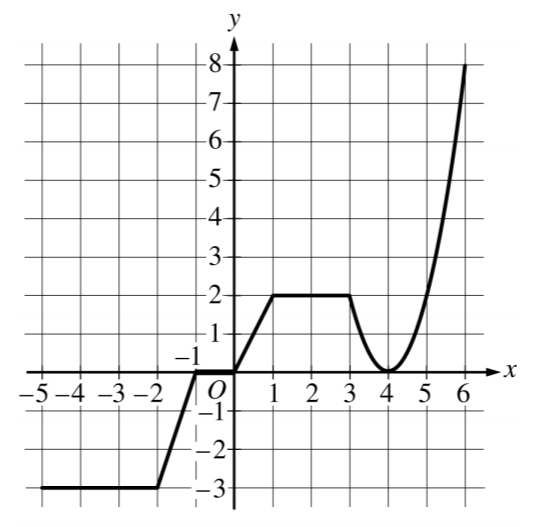
\includegraphics[width=0.5\textwidth]{./additional_materials/2018_3.png}
			\caption{\hyperref{https://apcentral.collegeboard.org/pdf/ap18-frq-calculus-bc.pdf}{}{}{AP Calculus BC 2018 Exam Free-Response Question 3, Graph of $g$}}
		\end{figure}
	
	\item
		The graph of the continuous function $g$, the derivative of a function $f$, is shown above.
		The function $g$ is piecewise linear for $-5 \leq x < 3$ and $g(x)=2(x-4)^2$ for $3 \leq x \leq 6$.
		\begin{enumerate}
			\item If $f(1)=3$, what is the value of $f(-5)$?
			\item Evaluate $\int_{1}^{6}{g(x)\d{x}}$.
			\item For $-5 < x < 6$, on what open intervals, if any, is the graph of $f$ both increasing and concave up?
				Give a reason for your answer.
			\item Find the $x$-coordinate of each point of inflection of the graph of $f$.
				Give a reason for your answer.
		\end{enumerate}
	
		\begin{table}[H]
			\begin{center}
				\begin{tabular}{|c||c|c|c|c|c|}
					\hline
					$t$ (years) & 2 & 3 & 5 & 7 & 10 \\
					\hline
					$H(t)$ (meters) & 1.5 & 2 & 6 & 11 & 15 \\
					\hline
				\end{tabular}
			\end{center}
		\end{table}
	
	\item The height of a tree at time $t$ is given by a twice-differentiable function $H$, where $H(t)$ is measured in meters and $t$ is measured in years.
		Selected values of $H(t)$ are given in the table above.
		\begin{enumerate}
			\item Use the data in the table to estimate $H^\prime(6)$.
				Using correct units, interpret the meaning of $H^\prime(6)$ in the context of the problem.
			\item Explain why there must be at least one time $t$, for $2 \leq t \leq 10$ such that $H^\prime(t) = 2$.
			\item Use a trapezoidal sum with 4 subintervals indicated by the data in the table to approximate the average height of the tree over the time interval $2 \leq 2 \leq 10$.
			\item The height of the tree, in meters, can also be modeled by the function $G$, given by $G(x)=\frac{100x}{1+x}$, where $x$ is the diameter of the base of the tree, in meters.
				When the tree is 50 meters tall, the diameter of the base of the tree is increasing at a rate of 0.03 meters per year.
				According to this model, what is the rate of the change of the height of the tree with respect to time, in meters per year, at the time when the tree is 50 meters tall?
		\end{enumerate}
	
	\begin{figure}[H]
		\label{2018_5}
		\centering
		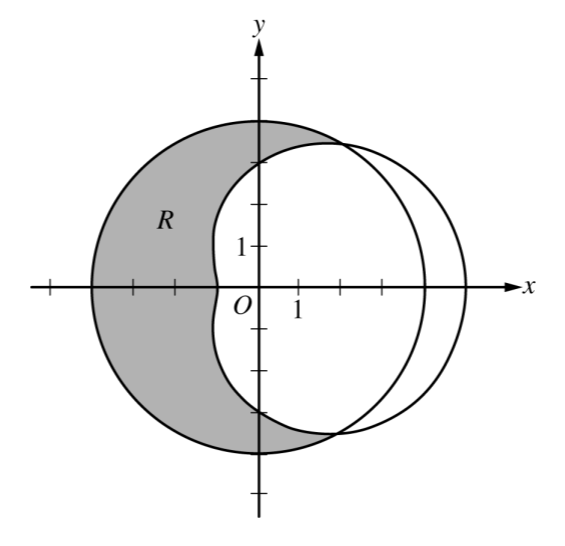
\includegraphics[width=0.5\textwidth]{./additional_materials/2018_5.png}
		\caption{\hyperref{https://apcentral.collegeboard.org/pdf/ap18-frq-calculus-bc.pdf}{}{}{AP Calculus BC 2018 Exam Free-Response Question 5}}
	\end{figure}
	
	\item The graph of the polar curves $r=4$ and $r=3+2\cos{\theta}$ are shown in the figure above.
		The curves intersect at $\theta = \frac{\pi}{3}$ and $\theta = \frac{5\pi}{3}$.
		\begin{enumerate}
			\item Let $R$ be the shaded region inside the graph of $r=4$ and outside the graph of $r=3+2\cos{\theta}$, as shown in the figure above.
				Write an expression involving an integral for the area of $R$.
			\item Find the slope of the line tangent to the graph $r=3+2\cos{\theta}$ at $\theta = \frac{\pi}{2}$.
			\item A particle moves along the portion of the curve  $r=3+2\cos{\theta}$ for $0 < \theta < \frac{\pi}{2}$.
				The particle moves in such a way that the distance between the particle and the origin increases at a constant rate of 3 units per second.
				Find the rate at which the angle $\theta$ changes with respect to time at the instant when the position of the particle corresponds to $\theta = \frac{\pi}{3}$.
				Indicate units of measure.
		\end{enumerate}
	
	\item The Maclaurin series for $\ln{(1+x)}$ is given by
		\begin{equation*}
			x - \frac{x^2}{2} + \frac{x^3}{3} - \frac{x^4}{4} + \ldots + (-1)^{n+1}\frac{x^n}{n} + \ldots .
		\end{equation*}
		On its interval of convergence, this series converges to $\ln{(1+x)}$.
		Let $f$ be a function defined by $f(x) = x\ln{\left(1+\frac{x}{3}\right)}$.
		\begin{enumerate}
			\item Write the first four nonzero erms and the general term of the Maclaurin series for $f$.
			\item Determine the interval of convergence for $f$.
				Show the work that leads to your answer.
			\item Let $P_4(x)$ be the fourth-degree Taylor polynomial for $f$ about $x=0$.
				Use the alternating series estimation bound to find an upper bound for $\abs{P_4(2)-f(2)}$.
		\end{enumerate}
	
\end{enumerate}
\subsection{2018 Free-Response Answers}
\begin{enumerate}
	\item \begin{enumerate}
		\item $r(t)$ tells us the rate at which people enter the line.
			By integrating $r(t)$ over the given interval, we can find the total number of people who entered the line.
			Using a calculator,
			\begin{equation*}
				\int_{0}^{300}{r(t)\d{t}} = \int_{0}^{300}{44\left(\frac{t}{100}\right)^3\left(1-\frac{t}{300}\right)^7\d{t}} = 270 \text{ people}.
			\end{equation*}
		\item We know that at $t=0$, there are already 20 people in line.
			Combining this fact with our answer from part (a), we know that $270+20=290$ people entered the line in the time interval.
			We also know that people leave the line at a constant rate of 0.7 people per second.
			Integrating this rate over the time interval will give us the number of people who left the line.
			\begin{equation*}
				\int_{0}^{300}{0.7\d{t}} = 210 \text{ people}.
			\end{equation*}
			So, there are $290-210=80$ people in line at $t=30$.
		\item We know from our answer in (b) that there are 80 people in line at $t=300$.
			We see from $r(t)$ that no more people are entering the line when $t>300$.
			So, the only thing that contributes to changing the number of people in line is people constantly leaving at a rate of 0.7 people per second.
			\begin{equation*}
				300\text{s} + \frac{80 \text{ people}}{0.7\text{ people/s}} \approx 414.286\text{s}.
			\end{equation*}
		\item Combining the fact that there are initially 20 people in line, the inflow rate is given by $r(t)$ and the outflow rate is 0.7, we can get that the number of people in line at time $x$ is modeled by
		\begin{equation*}
			20 + \int_{0}^{x}{\left(r(t)-0.7\right)\d{t}}.
		\end{equation*}
		Finding when the derivative is 0,
		\begin{equation*}
			r(t) - 0.7 = 0 \implies t = 33.013 \text{ or } 166.575.
		\end{equation*}
		Finding the number of people in line at these times and the endpoints 0 and 300,
		\begin{align*}
			\text{people}_{0} &= 20 \\
			\text{people}_{33.013} &= 3.803 \\
			\text{people}_{166.575} &= 158.070 \\
			\text{people}_{300} &= 80,
		\end{align*}
		we see that the fewest number of people occurs when $t\approx 33.013\text{s}$.
	\end{enumerate}

	\item \begin{enumerate}
		\item Using a calculator, we see that $p^\prime(25) = -1.17906$.
			In the context of the problem, this value means that at a depth of 25 meters, the density of plankton is decreasing at a rate of 1.17906 million plankton per cubic meter per meter.
		\item The vertical density of the plankton in the column is given by $p(h)*3\text{m}^2$.
			Integrating this density function for $0 \leq h \leq 30\text{m}$, we'll get the total number of plankton on the column.
			\begin{equation*}
				\int_{0}^{30}{3p(h)\d{h}} \approx 1675.414.
			\end{equation*}
			So, there are 1675.414 million plankton in the column from 0 to 30 meters depth.
		\item The total number of plankton in the entire vertical column with cross section area $A\text{m}^2$ is given by
			\begin{equation*}
				P = \int_{0}^{\infty}{A\text{density}(h)\d{h}}.
			\end{equation*}
			We can break this integral up, and we can use $A=3\text{m}^2$ for our particular column.
			\begin{equation*}
				P = 3\int_{0}^{30}{p(h)\d{h}} + 3\int_{30}^{\infty}{f(h)\d{h}}.
			\end{equation*}
			Since $u(h) \geq f(h)$ for $h \geq 30$, we can write the following inequality, the right side of which we can numerically evaluate:
			\begin{align*}
				P &\leq 3\int_{0}^{30}{p(h)\d{h}} + 3\int_{0}^{\infty}{u(h)\d{h}} \\
				&\leq 1675.414 + 3(105) \\
				&\leq 1990.414.
			\end{align*}
			So, we see that the number of plankton in the entire vertical column is at most 1990.414 million, which is strictly less than 2000 million.
		\item Since the position of the boat is parametric, we can use the parametric arc length formula to find the total distance traveled for $0 \leq t \leq 1\text{hr}$.
			\begin{align*}
				D &= \int_{0}^{1}{\sqrt{(x^\prime(t))^2+(y^\prime(t))^2}\d{t}} \\
				&= \int_{0}^{1}{\sqrt{\left(662\sin{(5t)}\right)^2 + \left(880\cos{(6t)}\right)^2}\d{t}} \\
				&\approx 757.456.
			\end{align*}
			So, for $0 \leq t \leq 1\text{hr}$, the boat travels a distance of 757.456 meters.
	\end{enumerate}

	\item \begin{enumerate}
		\item Trying to treat this like an initial value problem would be too tedious with all the piecewise parts of $g$.
			Plus, it would be doing more than the question asked because it only wants the value of $f$ at a particular point, not an expression for $f$.
			Instead, we can use the fact that $g$ is the derivative of $f$ and apply the Fundamental Theorem of Calculus.
			\begin{equation*}
				\int_{-5}^{1}{g(x)\d{x}} = f(1) - f(-5) = 3 - f(-5).
			\end{equation*}
			Evaluating the integral geometrically,
			\begin{equation*}
				\int_{-5}^{1}{g(x)\d{x}} = -(9+\frac{3}{2}) + 1 = \frac{-19}{2}.
			\end{equation*}
			Solving for $f(-5)$,
			\begin{equation*}
				\frac{-19}{2} = 3 - f(-5) \implies f(-5) = \frac{25}{2}.
			\end{equation*}
		\item Evaluating the integral,
			\begin{align*}
				\int_{1}^{6}{g(x)\d{x}} &= \int_{1}^{3}{2\d{x}} + \int_{3}^{6}{2(x-4)^2\d{x}} \\
				&= 2x\biggr\rvert_{1}^{3} + \frac{2}{3}(x-4)^3\biggr\rvert_{3}^{6} \\
				&= 4 + \frac{18}{3} \\
				&= 10.
			\end{align*}
		\item $f$ is increasing when its first derivative is positive and concave up when its second derivative is positive.
			Since $g$ is the derivative of $f$, we can also say that $f$ is increasing when $g$ is positive and concave up when $g$ is increasing.
			$g$ is positive on $(0,4) \cup (4,6]$.
			$g$ is increasing on $(-2,-1) \cup (0,1) \cup (4,6)$.
			Taking the intersection of these intervals, we see that $f$ is increasing and concave up on $(0,1) \cup (4,6)$.
		\item $f$ has an inflection point when its second derivative is equal to 0, changing sign.
			Since $g$ is the derivative of $f$, we can also say that $f$ has an inflection point when the derivative of $g$ is equal to 0, changing sign.
			Although we see by looking at the graph that the derivative of $g$ is 0 over several intervals, it does not change sign.
			The only place the derivative is 0 and changes sign is at $x=4$.
	\end{enumerate}

	\item \begin{enumerate}
		\item We can approximate $H^\prime(6)$ as the average rate of change between $t=5$ and $t=7$.
			\begin{equation*}
				H^\prime(6) \approx \frac{H(7)-H(5)}{7-5} = \frac{11-6}{7-5} = \frac{5}{2}.
			\end{equation*}
			In the context of this problem $H^\prime(6) \approx = \frac{5}{2}$ means that at 6 years, the tree is growing at a rate of 5/2 meters per year.
		\item Looking at the average rate of change between $t=3$ and $t=5$,
			\begin{equation*}
				\bar{H^\prime}_{3,5} = \frac{H(5)-H(3)}{5-3} = \frac{6-2}{5-3} = 2.
			\end{equation*}
			Since $H$ is differentiable, it is also continuous.
			So, by the mean value theorem, there is at least one point $3 \leq c \leq 5$ (which is a sub-interval of $2 \leq t \leq 10$) such that $H^\prime(c) = 2$. 
		\item We know that the average value of a continous function $f$ over some interval $[a,b]$ is
			\begin{equation*}
				\bar{f}_{a,b} = \frac{1}{b-a}\int_{a}^{b}{f(x)\d{x}}.
			\end{equation*}
			So, over our interval of $[2,10]$, we need to approximate this integral using trapezoids.
			Because the sub-interval widths given by the table are not equally-sized, we can't apply the shortcut trapezoidal rule.
			However, we can still approximate the area using trapezoids.
			\begin{equation*}
				\frac{1}{10-2}\int_{2}^{10}{H(x)\d{x}} \approx \frac{1}{8}\left(\frac{1.5+2}{2}1+\frac{2+6}{2}2+\frac{6+11}{2}2+\frac{11+15}{2}3\right) = \frac{1}{8}(65.75) = 8.21875.
			\end{equation*}
			So, the average height of the tree between 2 and 10 years is approximately 8.21875 meters.
		\item Finding the diameter of the base of the tree when it is 50 meters tall according to $G$.
			\begin{equation*}
				50 = \frac{100x}{1+x} \implies x = 1.
			\end{equation*}
			Differentiating $G$, remembering the chain rule,
			\begin{equation*}
				G^\prime(x) = \frac{100(1+x)\dd{x}{t} - 100x\dd{x}{t}}{(1+x)^2}.
			\end{equation*}
			Plugging in $x=1$ and $\dd{x}{t}=0.03$,
			\begin{equation*}
				G^\prime(1) = \frac{100(1+1)(0.03) - 100(1)(0.03)}{(1+1)^2} = \frac{6-3}{4} = \frac{3}{4}.
			\end{equation*}
			So, according to $G$, the tree is growing at 3/4 meters per year when it is 50 meters tall.
	\end{enumerate}

	\item \begin{enumerate}
		\item We know the formula for the area between two polar curves is
			\begin{equation*}
				A = \frac{1}{2}\int_{\alpha}^{\beta}{\left(f^2(\theta)-g^2(\theta)\right)\d{\theta}}.
			\end{equation*}
			Since we want the area inside the circle and outside the lima\c{c}on for $\pi/3 \leq \theta \leq 5\pi/3$,
			\begin{equation*}
				A = \frac{1}{2}\int_{\pi/3}^{5\pi/3}{\left((4)^2-(3+2\cos{\theta})^2\right)\d{\theta}}.
			\end{equation*}
		\item Remembering that $x=r\cos{\theta}$ and $y=r\sin{\theta}$,
			\begin{equation*}
				x = (3+2\cos{\theta})\cos{\theta} \text{, } y = (3+2\cos{\theta})\sin{\theta}.
			\end{equation*}
			Differentiating $x$ and $y$ with respect to $\theta$,
			\begin{equation*}
				\dd{x}{\theta}=-(3+2\cos{\theta})\sin{\theta} + \cos{\theta}(-2\sin{\theta}) \text{, } \dd{y}{\theta} = (3+2\cos{\theta})\cos{\theta} + \sin{\theta}(-2\sin{\theta}).
			\end{equation*}
			Dividing one by the other,
			\begin{equation*}
				\dd{y}{x} = \frac{\dd{y}{\theta}}{\dd{x}{\theta}} = \frac{(3+2\cos{\theta})\cos{\theta} + \sin{\theta}(-2\sin{\theta})}{-(3+2\cos{\theta})\sin{\theta} + \cos{\theta}(-2\sin{\theta})}.
			\end{equation*}
			At $\theta=\pi/2$,
			\begin{equation*}
				\dd{y}{x}_{\theta=\pi/2} = \frac{(3+2\cdot 0)\cdot 0 + 1(-2\cdot 1)}{-(3+2\cdot 0)1 + 0(-2\cdot 1)} = \frac{-2}{-3} = \frac{2}{3}.
			\end{equation*}
		\item $r$ is a function of $\theta$, and we're being told that $\theta$ behaves as a function of $t$, due to how the particle moves.
			So, we can apply the chain rule:
			\begin{align*}
				\dd{r}{t} &= \dd{r}{\theta}\cdot\dd{\theta}{t} \\
				&= -2\sin{\theta}\dd{\theta}{t}.
			\end{align*}
			Solving for $\dd{\theta}{t}$,
			\begin{equation*}
				\dd{\theta}{t} = \dd{r}{t}\frac{1}{-2\sin{\theta}}.
			\end{equation*}
			Moving away from the origin at some rate tell us how $r$ changes.
			Plugging in $\dd{r}{t}=3$ and $\theta=\pi/3$,
			\begin{equation*}
				\dd{\theta}{t} = 3\frac{1}{-2\sin{\left(\pi/3\right)}} = \frac{3}{-\sqrt{3}} = -\sqrt{3}.
			\end{equation*}
			So, $\theta$ is changing at a rate of $-\sqrt{3}$ radians per second.
	\end{enumerate}

	\item \begin{enumerate}
		\item Starting with the given Maclaurin series,
			\begin{equation*}
				\ln{(1+u)} = u - \frac{u^2}{2} + \frac{u^3}{3} - \frac{u^4}{4} + \ldots + (-1)^{n+1}\frac{u^n}{n} + \ldots .
			\end{equation*}
			Substituting $u=x/3$,
			\begin{equation*}
				\ln{\left(1+\frac{x}{3}\right)} = \frac{x}{3} - \frac{(\frac{x}{3})^4}{2} + \frac{(\frac{x}{3})^4}{3} - \frac{(\frac{x}{3})^4}{4} + \ldots + (-1)^{n+1}\frac{(\frac{x}{3})^n}{n} + \ldots .
			\end{equation*}
			Multiplying by $x$,
			\begin{equation*}
				x\ln{\left(1+\frac{x}{3}\right)} = x\frac{x}{3} - x\frac{(\frac{x}{3})^4}{2} + x\frac{(\frac{x}{3})^4}{3} - x\frac{(\frac{x}{3})^4}{4} + \ldots + (-1)^{n+1}x\frac{(\frac{x}{3})^n}{n} + \ldots .
			\end{equation*}
		\item Applying the ratio test on the absolute terms,
			\begin{equation*}
				\lim_{n\to\infty}{\frac{x\frac{(\frac{x}{3})^{n+1}}{n+1}}{x\frac{(\frac{x}{3})^n}{n}}} = \lim_{n\to\infty}{\frac{n\frac{x}{3}}{n+1}} = \frac{x}{3}.
			\end{equation*}
			The ratio test tells us the series converges when the limit is less than 1, so we can safely say that $\abs{x} < 3$, and we still need to test the endpoints.
			When $x=-3$ the series becomes
			\begin{equation*}
				\sum_{n=1}^{\infty}{(-1)^{n+1}(-3)\frac{\left(\frac{-3}{3}\right)^n}{n}} = \sum_{n=1}^{\infty}{\frac{3}{n}}
			\end{equation*}
			which diverges by the P-Test.
			When $x=3$, the series becomes
			\begin{equation*}
				\sum_{n=1}^{\infty}{(-1)^{n+1}3\frac{\left(\frac{3}{3}\right)^{n}}{n}} = \sum_{n=1}^{\infty}{(-1)^{n+1}\frac{3}{n}}
			\end{equation*}
			which converges by the Alternating Series Test.
			So, the interval of convergence is $-3 < x \leq 3$.
		\item The Alternating Series Estimation Theorem tells us that the error from an alternating series is at most the value of the first term not included, and the error is the same sign as the first not included term.
			For $P_4(x)$,
			\begin{equation*}
				\abs{P_4(2)-f(2)} \leq \abs{(-1)^5 2\frac{\left(\frac{2}{3}\right)^4}{4}} = \frac{8}{81}.
			\end{equation*}
			So, our upper bound on the error is $8/81$.
	\end{enumerate}
	
\end{enumerate}
\subsection{2017 Free-Response Questions}
Questions 1 and 2 are part of the same section and are allotted 30 minutes for completion with the aid of a graphing calculator.
Questions 3 through 6 are part of the same section and are allotted 1 hour for completion without the aid of a graphing calculator.

\begin{table}[H]
	\begin{center}
		\begin{tabular}{|c||c|c|c|c|}
			\hline
			$h$ (feet) & 0 & 2 & 5 & 10 \\
			\hline
			$A(h)$ (square feet) & 50.3 & 14.4 & 6.5 & 2.9 \\
			\hline
		\end{tabular}
	\end{center}
\end{table}

\begin{enumerate}
	
	\item A tank has a height of 10 feet.
		The are of the horizontal cross section of the tank at $h$ feet is given by the function $A$, where $A(h)$ is measured in square feet.
		The function $A$ is continuous and decreases as $h$ increases.
		Selected values for $h$ are given in the table above.
		\begin{enumerate}
			\item Use a left Riemann sum with three subintervals indicated by the data to approximate the volume of the tank.
				Indicate units of measure.
			\item Does the approximate in part (a) overestimate or underestimate the volume of the tank?
				Explain your reasoning.
			\item The area, in square feet, of the horizontal cross section at height $h$ feet is modeled by the function $f$ given by $f(h)=\frac{50.3}{e^{0.2h}+h}$.
				Based on this model, find the volume of the tank.
				Indicate units of measure.
			\item Water is pumped into the tank.
				When the height of the water is 5 feet, the height is increasing at a rate of 0.26 foot per minute.
				Using the model from part (c), find the rate at which the volume of water is changing with respect to time when the height of the water is 5 feet.
				Indicate units of measure.
		\end{enumerate}
	
	\begin{figure}[H]
		\label{2017_2}
		\centering
		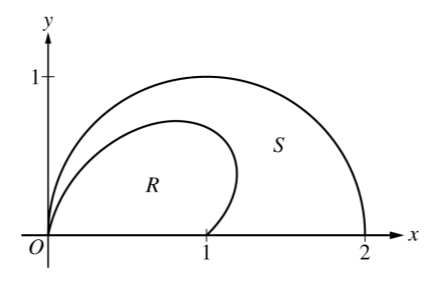
\includegraphics{./additional_materials/2017_2.png}
		\caption{\hyperref{https://apcentral.collegeboard.org/pdf/ap-calculus-bc-frq-2017.pdf}{}{}{AP Calculus BC 2017 Exam Free-Response Question 2}}
	\end{figure}

	\item The figure above show the polar curves $r=f(\theta)=1+\sin{\theta}\cos{(2\theta)}$ and $r=g(\theta)=2\cos{\theta}$ for $0 \leq \theta \leq \frac{\pi}{2}$.
		Let $R$ be the region in the first quadrant bounded by the curve $r=f(\theta)$ and the $x$-axis.
		Let $S$ be the region in the first quadrant bounded by the curve $r=f(\theta)$ the curve $r=g(\theta)$, and the $x$-axis.
		\begin{enumerate}
			\item Find the area of $R$.
			\item The ray $\theta = k$, where $0 < k < \frac{\pi}{2}$, divides $S$ into two regions of equal area.
				Write out, but do not solve, an equation involving one or more integrals whose solution gives the value of $k$.
			\item For each $\theta$, $0 \leq \theta \leq \frac{\pi}{2}$, let $w(\theta)$ be the distance between the points with polar coordinates $(f(\theta),\theta)$ and $(g(\theta),\theta)$.
				Write an expression for $w(\theta)$.
				Find $w_A$, the average value of $w(\theta)$ over the interval $0 \leq \theta \leq \frac{\pi}{2}$.
			\item Using the information given from part (c), find the value of $\theta$ for which $w(\theta)=w_A$.
				Is the function $w(\theta)$ increasing or decreasing at that value of $\theta$?
				Give a reason for your answer.
		\end{enumerate}
	
	\begin{figure}[H]
		\label{2017_3}
		\centering
		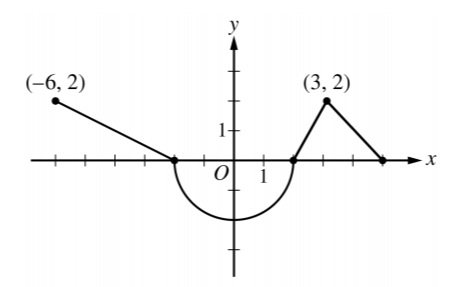
\includegraphics{./additional_materials/2017_3.png}
		\caption{\hyperref{https://apcentral.collegeboard.org/pdf/ap-calculus-bc-frq-2017.pdf}{}{}{AP Calculus BC 2017 Exam Free-Response Question 3, Graph of $f^\prime$}}
	\end{figure}
	
	\item The function $f$ is differentiable on the closed interval $[-6,5]$ and satisfies $f(-2)=7$.
		The graph of $f^\prime$, the derivative of $f$, consists of a semicircle and three line segments, as shown in the figure above.
		\begin{enumerate}
			\item Find the values of $f(-6)$ and $f(5)$.
			\item On what intervals is $f$ increasing?
				Justify your answer.
			\item Find the absolute minimum value of $f$ on the closed interval $[-6,5]$.
				Justify your answer.
			\item For each of $f^{\prime\prime}(-5)$ and $f^{\prime\prime}(3)$, find the value or explain why it doesn't exist.
		\end{enumerate}
	
	\item At time $t=0$, a boiled potato is taken from a pot on a stove and left to cool in a kitchen.
		The internal temperature of the potato is 91 degrees Celsius ($^\circ C$) at time $t=0$, and the internal temperature of the potato is greater than $27^\circ C$ for all time $t > 0$.
		The internal temperature of the potato at time $t$ minutes can be modeled by a function $H$ that satisfies the differential equation $\dd{H}{t} = -\frac{1}{4}(H-27)$, where $H(t)$ is measured in degrees Celsius and $H(0)=91$.
		\begin{enumerate}
			\item Write an equation for the line tangent to the graph of $H$ at $t=0$.
				Use this equation to approximate the internal temperature of the potato at time $t=3$.
			\item Use $\dd{^2H}{t^2}$ to determine whether your answer in part (a) is an underestimate or overestimate of the internal temperature of the potato at time $t=3$.
			\item For $t<10$, an alternate model for the internal temperature of the potato at time $t$ minutes is the function $G$ that satisfies the differential equation $\dd{G}{t} = -(G-27)^{2/3}$, where $G(t)$ is measured in degrees Celsius and $G(0)=91$.
				Based on this model, what is the internal temperature of the potato at time $t=3$?
		\end{enumerate}
	
	\item Let $f$ be the function defined by $f(x) = \frac{3}{2x^2-7x+5}$.
		\begin{enumerate}
			\item Find the slope of the tangent line of the graph of $f$ at $x=3$.
			\item Find the $x$-coordinate of each critical point of $f$ in the interval $1 < x < 2.5$.
				Classify each critical point as the location of a relative minimum, a relative maximum, or neither.
				Justify your answer.
			\item Using the identity that $\frac{3}{2x^2-7x+5} = \frac{2}{2x-5} - \frac{1}{x-1}$, evaluate $\int_{5}^{\infty}{f(x)\d{x}}$ or show that the integral diverges.
			\item Determine whether the series $\sum_{n=5}^{\infty}{\frac{3}{2n^2-7n+5}}$ converges or diverges.
				State the conditions of the test used for determining convergence or divergence.
		\end{enumerate}
	
	\begin{align*}
		f(0) &= 0 \\
		f^\prime(0) &= 1 \\
		f^{(n+1)}(0) &= -n\cdot f^{(n)}(0) \text{ for all } n \geq 1
	\end{align*}
	
	\item A function $f$ has derivatives of all order for $-1 < x < 1$.
		The derivatives of $f$ satisfy the conditions above.
		The Maclaurin Series for $f$ converges to $f(x)$ for $\abs{x} < 1$.
		\begin{enumerate}
			\item Show that the first four non-zero terms of the Maclaurin series for $f$ are $x - \frac{x^2}{2} + \frac{x^3}{3} - \frac{x^4}{4}$, and write the general term for the Maclaurin series for $f$.
			\item Determine whether the Maclaurin series described in part (a) converges absolutely, converges conditionally, or diverges at $x=1$.
				Explain your reasoning.
			\item Write the first four nonzero terms and the general term for the Maclaurin series for $g(x) = \int_{0}^{x}{f(t)\d{t}}$.
			\item Let $P_n\left(\frac{1}{2}\right)$ represent the $n$th degree Taylor polynomial for $g$ about $x=0$ and evaluated at $x=\frac{1}{2}$, where $g$ is the function defined in part (c).
				Use the alternating series error bound to show that
				\begin{equation*}
					\biggr\lvert P_4\left(\frac{1}{2}\right) - g\left(\frac{1}{2}\right) \biggr\rvert < \frac{1}{500}.
				\end{equation*}
		\end{enumerate}
	
\end{enumerate}
\subsection{2017 Free-Response Answers}

\begin{enumerate}
	\item \begin{enumerate}
		\item Using a left Riemann sum,
			\begin{equation*}
				\int_{0}^{10}{A(h)\d{h}} \approx (2-0)50.3 + (5-2)14.4 + (10-5)6.5 = 100.6 + 43.2 + 32.5 = 176.3.
 			\end{equation*}
 			So, we approximate that the volume of the tank is 176.3 cubic feet.
 		\item Since we are given that the function is decreasing over the interval, a left Riemann sum will overestimate the volume.
 		\item Integrating $f$ from $h=0$ to $h=10$,
 			\begin{equation*}
 				\int_{0}^{10}{\frac{50.3}{e^{0.2h}+h}\d{h}} \approx 101.325.
 			\end{equation*}
 			So, the volume of the tank given by $f$ is 101.325 cubic feet.
 		\item We know from (c) that
 			\begin{equation*}
 				V(h) = \int_{0}^{h}{f(x)\d{x}}.
 			\end{equation*}
 			Differentiating with respect to $t$, and applying the chain rule,
 			\begin{equation*}
 				\dd{V}{t} = f(h)\cdot\dd{h}{t}.
 			\end{equation*}
 			Plugging in $h=5$ and $\dd{h}{t}=0.26$,
 			\begin{equation*}
 				\dd{V}{t}_{h=5} = \frac{50.3}{e^1 + 5}\cdot 0.26 \approx 1.694.
 			\end{equation*}
 			So, when $h=5$ feet, the volume is changing at a rate of 1.694 cubic feet per minute.
	\end{enumerate}

	\item \begin{enumerate}
		\item Finding the area enclosed by $f$ from $\theta=0$ to $\theta=\pi/2$,
			\begin{equation*}
				A = \frac{1}{2}\int_{0}^{\pi/2}{\left(1+\sin{\theta}\cos{(2\theta)}\right)^2d\theta} \approx 0.648.
			\end{equation*}
		\item Our ray $\theta=k$ will represent a lower bound in one integral and an upper bound in the other.
			Finding equal areas between $g$ and $f$,
			\begin{equation*}
				\frac{1}{2}\int_{0}^{k}{\left(\left(2\cos{\theta}\right)^2-\left(1+\sin{\theta}\cos{(2\theta)}\right)^2\right)d\theta} = \frac{1}{2}\int_{k}^{\pi/2}{\left(\left(2\cos{\theta}\right)^2-\left(1+\sin{\theta}\cos{(2\theta)}\right)^2\right)d\theta}.
			\end{equation*}
		\item
			Since both $f$ and $g$ are polar functions evaluated at $\theta$, the distance between then will simply be the difference in their radii.
			\begin{equation*}
				w(\theta) = g(\theta) - f(\theta).
			\end{equation*} 
			Finding the average of $w$,
			\begin{equation*}
				w_A = \frac{1}{\pi/2 - 0}\int_{0}^{\pi/2}{(2\cos{\theta}-(1+\sin{\theta}\cos{(2\theta)}))\d{\theta}} \approx 0.485.
			\end{equation*}
		\item Solving $w(\theta) = w_A$,
			\begin{equation*}
				2\cos{\theta}-(1+\sin{\theta}\cos{(2\theta)}) = 0.485 \implies \theta \approx 0.518.
			\end{equation*}
			Evaluating $w^\prime(0.518)$,
			\begin{equation*}
				w^\prime(0.518) \approx -0.581.
			\end{equation*}
			So, $w$ is decreasing at this value.
	\end{enumerate}

	\item \begin{enumerate}
		\item Applying the Fundamental Theorem of Calculus,
			\begin{align*}
				\int_{-6}^{-2}{f^\prime(x)\d{x}} &= f(-2) - f(-6) = 7 - f(-6) = 4 \implies f(-6) = 3 \\
				\int_{-2}^{5}{f^\prime(x)\d{x}} &= f(5) - f(-2) = f(5) - 7 = -2\pi + 3 \implies f(5) = 10 - 2\pi.
			\end{align*}
		\item $f$ is increasing when its derivative is positive.
			Looking at the graph of $f^\prime$, we see it is positive on $[-6,2) \cup (2,5)$.
			So, $f$ is increasing on $[-6,2] \cup [2,5]$\footnote{I personally don't think $f$ is ``increasing" on the open endpoints where the derivative is 0. I think it's neither increasing nor decreasing. However, the test writers and graders feel differently, and I can't say their view is necessarily wrong.}.
		\item We see that the critical points of $f^\prime$ are $x=-2$ and $x=2$.
			A minimum can occur at a left/right endpoint that will/was decreasing.
			So, the two points we need to consider for the absolute minimum are $x=-6$ and $x=2$.
			We know from (a) that $f(-6)=3$.
			Applying the Fundamental Theorem of Calculus again,
			\begin{equation*}
				\int_{-2}^{2}{f^\prime(x)\d{x}} = f(2) - f(-2) = f(2) - 7 = 2\pi \implies f(2) = 7-2\pi.
			\end{equation*}
			Since  $7-2\pi < 3$, the absolute minimum of $f$ is at $x=2$.
		\item $f^{\prime\prime}(-5) = -\frac{1}{2}$ because $f$ is continuous at -5, and the left and right hand limits are both the slope of the line, which is $-\frac{1}{2}$.
			$f^{\prime\prime}(3) = \text{DNE}$.
			The left hand limit is the slope of the left hand line, which is 2, and the right hand limit is the left of the right hand line, which is -1.
			Since the limits do not agree, $f^\prime$ is not continuous, and hence not differentiable at $x=3$.
	\end{enumerate}

	\item \begin{enumerate}
		\item Writing the line in point-slope form and then converting to standard form,
			\begin{align*}
				y - y_0 &= m(t-t_0) \\
				y - H(0) &= \dd{H}{t}_{t=0}(t-0) \\
				y - 91 &= -16t \\
				y &= -16t + 91.
			\end{align*}
			Using this line to approximate $H(3)$,
			\begin{equation*}
				y = -16(3) + 91 = 43.
			\end{equation*}
			So, the tangent line at $t=0$ approximates $H(3)$ to be $43^\circ C$.
		\item Taking the derivative of $\dd{H}{t}$,
			\begin{equation*}
				\dd{^2H}{t^2} = -\frac{1}{4}.
			\end{equation*}
			Since the graph is concave down at every point, the tangent line at $t=0$ gives an overestimate of $H(3)$.
		\item This is a separable differential equation.
			\begin{align*}
				\dd{G}{t} &= -(G-27)^{2/3} \\
				\frac{\d{G}}{(G-27)^{2/3}} &= -1\d{t} \\
				\int{\frac{\d{G}}{(G-27)^{2/3}}} &= \int{-1\d{t}} \\
				3(G-27)^{1/3} &= -t + C \\
				(G-27)^{1/3} &= -t/3 + C \\
				G - 27 &= \left(-t/3 + C\right)^3 \\
				G &= \left(-t/3 + C\right)^3 + 27.
			\end{align*}
			Solving for $C$ using $G(0)=91$,
			\begin{align*}
				91 &= \left(-0/3 + C\right)^2 + 27 \\
				64 &= C^3 \\
				C &= 4.
			\end{align*}
			So, our overall solution for $G$ is
			\begin{equation*}
				G(t) = \left(4 - t/3\right)^3 + 27.
			\end{equation*}
			Evaluating at $t=3$,
			\begin{equation*}
				G(3) = \left(4 - 3/3\right)^3 + 27 = 3^3  + 27 = 54.
			\end{equation*}
			So, the internal temperature of the potato at $t=3$ minutes is $54^\circ C$.
	\end{enumerate}

	\item \begin{enumerate}
		\item Applying the quotient rule,
			\begin{equation*}
				f^\prime(x) = \frac{(2x^2-7x+5)(0)-3(4x-7)}{(2x^2-7x+5)^2} = \frac{-12x+21}{(2x^2-7x+5)^2}.
			\end{equation*}
			Evaluating at $x=3$,
			\begin{equation*}
				f^\prime(3) = \frac{-12(3)+21}{(2(3)^2-7(3)+5)^2} = -\frac{15}{(18-21+5)^2} = -\frac{15}{4}.
			\end{equation*}
		\item $f^\prime(x)=0$ only when the numerator is 0,
			\begin{equation*}
				-12x + 21 = 0 \implies x = \frac{7}{4}.
			\end{equation*}
			$f^\prime$ is negative to the left of $\frac{7}{4}$ and positive to the right of it.
			Therefore, $x=\frac{7}{4}$ is a relative maximum by the first derivative test.
		\item Evaluating the limit using the given partial fraction decomposition,
			\begin{align*}
				\int_{5}^{\infty}{f(x)\d{x}} &= \int_{5}^{\infty}{\left(\frac{2}{2x-5}-\frac{1}{x-1}\right)\d{x}} \\
				&= \ln{(2x-5)} - \ln{(x-1)} \biggr\rvert_{5}^{\infty} \\
				&= \ln{\left(\frac{2x-5}{x-1}\right)} \biggr\rvert_{5}^{\infty} \\
				&= \lim_{b\to\infty}{\ln{\left(\frac{2b-5}{b-1}\right)}} - \ln{\left(\frac{5}{4}\right)} \\
				&= \ln{2} - \ln{\left(\frac{5}{4}\right)} \\
				&= \ln{\left(\frac{8}{5}\right)}.
			\end{align*}
		\item For $n \geq 5$, $f(n)$ is positive and decreasing.
			Using our work from part (c), we know that the integral of $f$ from 5 to $\infty$ converges.
			So, by the Integral test, the series also converges.
	\end{enumerate}

	\item \begin{enumerate}
		\item Calculating the first four derivatives and the general derivative,
			\begin{align*}
				f(0) &= 0 \\
				f^\prime(0) &= 1 \\
				f^{\prime\prime}(0) &= -1\cdot f^\prime(0) = -1 \\
				f^{(3)}(0) &= -2\cdot f^{\prime\prime}(0) = 2 \\
				f^{(4)}(0) &= -3\cdot f^{(3)}(0) = -6.
				f^{(n+1)}(0) &= -n\cdot f^{(n)}(0) = (-1)^{n+1}n!.
			\end{align*}
			Applying the Maclaurin series formula,
			\begin{align*}
				P_n(x) &= \frac{f(0)}{0!} + \frac{f^\prime(0)}{1!}x + \frac{f^{\prime\prime}(0)}{2!}x^2 + \ldots + \frac{f^{(n)}(0)}{n!}x^n \\
				&= \frac{0}{1} + \frac{1}{1}x + \frac{-1}{2}x^2 + \frac{2}{6}x^3 + \frac{-6}{24}x^4 + \ldots + \frac{(-1)^{n+1}(n-1)!}{n!}x^n \\
				&= x - \frac{x^2}{2} + \frac{x^3}{3} - \frac{x^4}{4} + \ldots + (-1)^{n+1}\frac{x^n}{n}.
			\end{align*}
		\item At $x=1$, the series is
			\begin{equation*}
				\sum_{n=1}^{\infty}{(-1)^{n+1}\frac{1}{n}}.
			\end{equation*}
			This series converges by the Alternating Series test, which determines conditional converges.
			So, the series converges conditionally at $x=1$.
		\item Integrating term-by-term,
			\begin{align*}
				g(x) &= \int_{0}{x}{f(t)\d{t}} \\
				&= \int_{0}^{x}{\left(t-\frac{t^2}{2}+\frac{t^3}{3}-\frac{t^4}{4}+\ldots+(-1)^{n+1}\frac{t^n}{n}\right)\d{t}} \\
				&= \frac{t^2}{2} - \frac{t^3}{6} + \frac{t^4}{12} - \frac{t^5}{20} + \ldots + (-1)^{n+1}\frac{t^{n+1}}{n(n+1)} \biggr\rvert_{0}^{x} \\
				&= \frac{x^2}{2} - \frac{x^3}{6} + \frac{x^4}{12} - \frac{x^5}{20} + \ldots + (-1)^{n+1}\frac{x^{n+1}}{n(n+1)}.
			\end{align*}
		\item The Alternating Series Estimation Theorem tells us that the upper bound for the error is the absolute value of the first not included term.
			For $P_4$, this term is $-\frac{x^5}{20}$.
			So,
			\begin{align*}
				\biggr\lvert P_4\left(\frac{1}{2}\right) - g\left(\frac{1}{2}\right) \biggr\rvert < \biggr\lvert -\frac{\left(\frac{1}{2}\right)^5}{20} \biggr\rvert = \frac{1}{640} < \frac{1}{500}.
			\end{align*}
	\end{enumerate}

\end{enumerate}
\subsection{2016 Free-Response Questions}
Questions 1 and 2 part of the same section area are allotted 30 minutes from completion with the aid of a graphing calculator.
Questions 3 through 6 are part of the same section and area allotted 1 hour from completion without the aid of a graphing calculator.

\begin{table}[H]
	\begin{center}
		\begin{tabular}{|c||c|c|c|c|c|}
			\hline
			$t$ (hours) & 0 & 1 & 3 & 6 & 8 \\
			\hline
			$R(t)$ (liters / hour) & 1340 & 1190 & 950 & 740 & 700 \\
			\hline
		\end{tabular}
	\end{center}
\end{table}

\begin{enumerate}
	\item Water is pumped into a tank at a rate modeled by $W(t)=2000e^{-t^2/20}$ liters per hour for $0 \leq t \leq 8$, where $t$ is measured in hours.
	Water is removed from the tank at a rate modeled by $R(t)$ liters per hour, where $R$ is differentiable and decreasing on $0 \leq t \leq 8$.
	Selected values of $R(t)$ are shown in the table above.
	At time $t=0$, there are 50000 liters of water in the tank.
	\begin{enumerate}
		\item Estimate $R^\prime(2)$.
		Show the work that leads to your answer.
		Indicate units of measure.
		\item Use a left Riemann sum with the four subintervals indicated by the table to estimate the total amount of water removed from the tank during the 8 hours.
		Is this an over estimate or underestimate of the total amount of water removed?
		Give a reason for your answer.
		\item Use your answer from part (b) to find an estimate for the total amount of water in the tank, to the nearest liters, at the end of the 8 hours.
		\item For $0 \leq t \leq 8$, is there a time $t$ when the rate at which the water is pumped into the tank is the same rate as the rate at which water is removed from the tank?
		Explain why or why not.
	\end{enumerate}

	\begin{figure}[H]
		\label{2016_2}
		\centering
		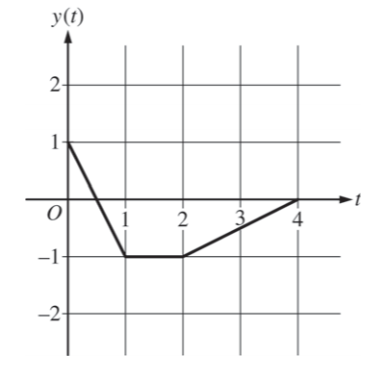
\includegraphics{./additional_materials/2016_2.png}
		\caption{\hyperref{https://secure-media.collegeboard.org/digitalServices/pdf/ap/ap16\_frq\_calculus\_bc.pdf}{}{}{AP Calculus BC 2016 Exam Free-Response Question 2}}
	\end{figure}
	
	\item At time $t$, the position of a particle moving in the $xy$-plane is given by the parametric functions $(x(t),y(t))$, where $\dd{x}{t} = t^2 + \sin{(3t^2)}$.
		The graph of $y$ consisting of three line segments, is shown in the figure above.
		At $t=0$, the particle is at position $(5,1)$.
		\begin{enumerate}
			\item Find the position of the particle at $t=3$.
			\item Find the slope of the line tangent to the part of the particle at $t=3$.
			\item Find the speed of the particle at $t=3$.
			\item Find the total distance traveled by the particle from $t=0$ to $t=2$.
		\end{enumerate}
	
	\begin{figure}[H]
		\label{2016_3}
		\centering
		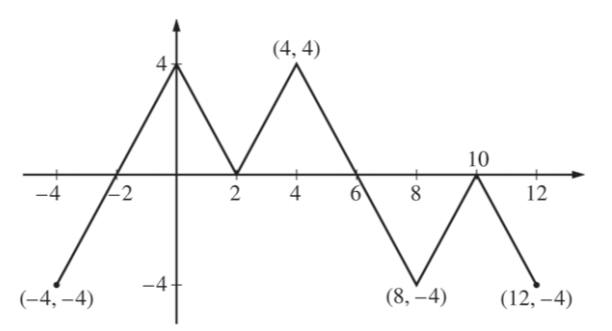
\includegraphics{./additional_materials/2016_3.png}
		\caption{\hyperref{https://secure-media.collegeboard.org/digitalServices/pdf/ap/ap16\_frq\_calculus\_bc.pdf}{}{}{AP Calculus BC 2016 Exam Free-Response Question 3, Graph of $f$}}
	\end{figure}
	
	\item The figure above shows the graph of the piecewise-linear function $f$.
		For $-4 \leq x \leq 12$, the function $g$ is defined by $g(x)=\int_{2}^{x}{f(t)\d{t}}$.
		\begin{enumerate}
			\item Does $g$ have a relative minimum, a relative maximum, or neither at $x=10$?
				Justify your answer.
			\item Does the graph of $g$ have a point of inflection at $x=4$?
				Justify your answer.
			\item Find the absolute minimum value and the absolute maximum value of $g$ on the interval $-4 \leq x \leq 12$.
				Justify your answers.
			\item For $-4 \leq x \leq 12$, find all intervals for which $g(x) \leq 0$.
		\end{enumerate}
	
	\item Consider the differential equation $\dd{y}{x} = x^2 - \frac{1}{2}y$.
		\begin{enumerate}
			\item Find $\dd{^2y}{x^2}$ in terms of $x$ and $y$.
			\item Let $y=f(x)$ be the particular solution to the given differential equation whose graph passes through the point $(-2,8)$.
				Does the graph of $f$ have a relative minimum, a relative maximum, or neither at the point $(-2,8)$?
				Justify your answer.
			\item Let $y=g(x)$ be the particular solution to the given differential equation with $g(-1)=2$.
				Find $\lim_{x\to -1}{\left(\frac{g(x)-2}{3(x+1)^2}\right)}$.
				Show the work that leads to your answer.
			\item Let $y=h(x)$ be the particular solution to the given differential equation with $h(0)=2$.
				Use Euler's method, starting at $x=0$ with two steps of equal size, to approximate $h(1)$.
		\end{enumerate}
	
	\begin{figure}[H]
		\label{2016_5}
		\centering
		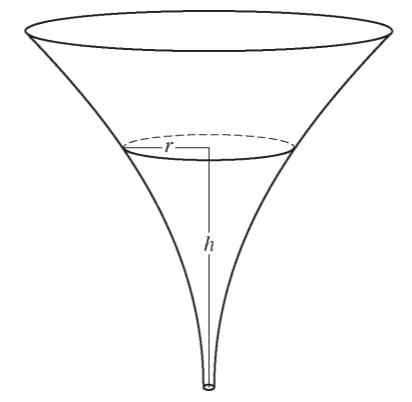
\includegraphics{./additional_materials/2016_5.png}
		\caption{\hyperref{https://secure-media.collegeboard.org/digitalServices/pdf/ap/ap16\_frq\_calculus\_bc.pdf}{}{}{AP Calculus BC 2016 Exam Free-Response Question 5}}
	\end{figure}
	
	\item The inside of a funnel of height 10 inches has circular cross sections, as shown in the figure above.
		At height $h$, the radius of the funnel is given by $r = \frac{1}{20}\left(3+h^2\right)$, where $0 \leq h \leq 10$.
		The units of $r$ and $h$ are inches.
		\begin{enumerate}
			\item Find the average value of the radius of the funnel.
			\item Find the volume of the funnel.
			\item The funnel contains liquid that is draining from the bottom.
				At the instant when the height of the liquid is $h=3$ inches, the radius of the surface of the liquid is decreasing at a rate of $\frac{1}{5}$ inch per second.
				At this instant, what is the rate of change of the height of the liquid with respect to time?
		\end{enumerate}
	
	\item The function $f$ has a Taylor series about $x=1$ that converges to $f(x)$ for all $x$ in the interval of convergence.
		It is known that $f(1)=1$, $f^\prime(1)=-\frac{1}{2}$, and the $n$th derivative of $f$ at $x=1$ is given by $f^{(n)}(1) = (-1)^{n}\frac{(n-1)!}{2^n}$ for $n \geq 2$.
		\begin{enumerate}
			\item Write the first four nonzero terms and the general term of the Taylor series for $f$ about $x=1$.
			\item The Taylor series for $f$ about $x=1$ has a radius of convergence of 2.
				Find the interval of convergence.
				Show the work that leads to your answer.
			\item The Taylor series for $f$ about $x=1$ can be used to represent $f(1.2)$ as an alternating series.
				Use the first three non-zero terms of the alternating series to approximate $f(1.2)$.
			\item Show that the approximation found in part (c) is within 0.001 of the exact value of $f(1.2)$.
		\end{enumerate}
\end{enumerate}
\subsection{2016 Free-Response Answers}

\begin{enumerate}
	\item \begin{enumerate}
		\item We can approximate $R^\prime(2)$ as the tangent slope between 1 and 3.
			\begin{equation*}
				R^\prime(2) \approx \frac{R(3)-R(1)}{3-1} = \frac{950-1190}{2} = -120.
			\end{equation*}
			So, we estimate $R^\prime(3)$ to be -120 liters/hour$^2$.
		\item Using a left Riemann sum using the values in the table,
			\begin{equation*}
				\int_{0}^{8}{R(t)\d{t}} \approx (1-0)1340 + (3-1)1190 + (6-3)950 + (8-6)740 = 1340 + 2380 + 2850 + 1480 = 8050.
			\end{equation*}
			So, the left Riemann sum approximates the total water removed to be 8050 liters.
		\item Using our answer from part (b) and integrating, we can find the total amount of water added or removed.
			\begin{equation*}
				\Delta \text{Water} = -8050 + \int_{0}{8}{2000e^{-t^2/20}\d{t}} \approx -214.
			\end{equation*}
			Since we know there is 50000 liters of water at $t=0$, we can add the net change to find the amount of water at $t=8$.
			\begin{equation*}
				\text{Water}_8 = \text{Water}_0 + \Delta \text{Water} = 50000 - 214 = 49768.
			\end{equation*}
			So, to the nearest liter, we approximate the amount of water in the tank at $t=8$ to be 49768 liters.
		\item At $t=0$, $W(0) = 2000 > R(0) = 1340$, so $W(0)-R(0) > 0$.
			At $t=8$, $W(8) = 81.52 < R(8) = 700$, so $W(8)-R(8) < 0$.
			Since both $W$ and $R$ are continuous, so is $W - R$.
			So, by the Intermediate Value Theorem, there is some $0 < t < 8$ such that $W(t)-R(t)=0$, or $W(t)=R(t)$.
	\end{enumerate}

	\item \begin{enumerate}
		\item We can apply the Fundamental Theorem of Calculus to find $x(3)$.
			\begin{equation*}
				\int_{0}^{3}{\dd{x}{t}\d{t}} = x(3) - x(0) = x(3) - 5 = 9.377 \implies x(3) = 14.377.
			\end{equation*}
			Looking at the graph, we see that $y(3)=-\frac{1}{2}$.
			So, at $t=3$, the particle's position is $\left(14.377, -0.5\right)$.
		\item Looking at the graph, we see that $y^\prime(3) = \frac{1}{2}$.
			Evaluating $\dd{x}{t}$ at $t=3$, we see that $x^\prime(3) = 9+\sin{27}$.
			So,
			\begin{equation*}
				\dd{y}{x} = \frac{\dd{y}{t}}{\dd{x}{t}} = \frac{\frac{1}{2}}{9+\sin{27}} \approx 0.0502.
			\end{equation*}
		\item Using our formula for parametric speed,
			\begin{equation*}
				s = \sqrt{(x^\prime(t))^2 + (y^\prime(t))^2} = \sqrt{\left(\frac{1}{2}\right)^2 + \left(9+\sin{27}\right)^2} \approx 9.969.
			\end{equation*}
		\item Starting with the formula for parametric arc length and splitting the integral into two peices,
			\begin{align*}
				\int_{0}^{2}{\sqrt{\left(y^\prime(t)\right)^2+\left(x^\prime(t)\right)^2}\d{t}} &= \int_{0}^{1}{\sqrt{(-2)^2+(t^2+\sin{(3t^2)})^2}\d{t}} + \int_{1}^{2}{\sqrt{(0)^2+(t^2+\sin{(3t^2)})^2}\d{t}} \\
				&\approx 2.237 + 2.112 \\
				&= 4.439.
			\end{align*}
	\end{enumerate}

	\item \begin{enumerate}
		\item Since we know by the Fundamental Theorem of Calculus that $f$ is the derivative of $g$, $g$ has critical points where $f$ is 0.
			$x=10$ is one such critical point.
			Both to the left and right of $x=10$, $f$ is negative.
			So, although $x=10$ is a critical point, it is neither a relative minimum or relative maximum of $g$ because $g$ is decreasing both left and right of $x=10$.
		\item Inflection points occur when the second derivative changes sign.
			Since $f$ is the derivative of $g$, inflection points of $g$ occur when the derivative of $f$ changes sign.
			To the left of $x=4$, the derivative of $f$ is positive.
			To the right of $x=4$, the derivative of $f$ is negative.
			So, $x=4$ is indeed an inflection point for $g$.
		\item $g$ has critical points where $f$ is 0, which is at $x=-2$, $x=2$, $x=6$, and $x=10$.
			Of these, $x=2$ and $x=10$ do not change sign, so they cannot be absolute extrema.
			Evaluating the remaining critical points and the endpoints using the geometry of the graph of $f$,
			\begin{align*}
				g(-4) &= -4 \\
				g(-2) &= -8 \\
				g(6) &= 8 \\
				g(12) &= -4.
			\end{align*}
			So, the absolute minimum of $g$ is at $x=-2$, and the absolute maximum of $g$ is at $x=6$.
		\item To the left $x=2$, $g(x)$ is negative whenever there is more area between $f$ and the $x$-axis above the $x$-axis than below.
			So, all points $[-4,2]$ have $g(x) \leq 0$.
			To the left of $x=2$, the opposite is true.
			So, all points $[10,12]$ have $g(x) \leq 0$.
			Putting these two results together, $g(x) \leq 0$ on $[-4,2] \cup [10,12]$. 
	\end{enumerate}

	\item \begin{enumerate}
		\item Implicitly differentiating,
			\begin{equation*}
				\d{^2y}{x^2} = 2x - \frac{1}{2}\dd{y}{x} = 2x - \frac{1}{2}\left(x^2 - \frac{1}{2}y\right).
			\end{equation*}
		\item Since we have expression for the first and second derivatives, it makes the most sense to apply a second derivative test.
			First, checking that $(-2,8)$ is indeed a critical point,
			\begin{equation*}
				\dd{y}{x}_{(-2,8)} = (-2)^2 - \frac{1}{2}(8) = 0.
			\end{equation*}
			Next, evaluating the second derivative,
			\begin{equation*}
				\dd{^2y}{x^2}_{(-2,8)} = 2(-2) - \frac{1}{2}\left((-2)^2 - \frac{1}{2}(8)\right) = -4 - 0 = -4.
			\end{equation*}
			Since the second derivative is negative at this critical point, the second derivative test tells us that this is a relative maximum.
		\item Since we know that $g(-1)=2$, both the numerator and denominator of the limit are in an indeterminate form of 0/0.
			So, we can apply L'H\^{o}pital's Rule.
			\begin{equation*}
				\lim_{x\to -1}{\left(\frac{g(x)-2}{3(x+1)^2}\right)} = \lim_{x\to-1}\left(\frac{g^\prime(x)}{6(x+1)}\right).
			\end{equation*}
			Using the given differential equation, we can see that at $(-1,2)$, $g^\prime(-1)=0$.
			So again we have an indeterminate form of 0/0 and can apply L'H\^{o}pital's Rule.
			\begin{equation*}
				\lim_{x\to-1}\left(\frac{g^\prime(x)}{6(x+1)}\right) = \lim_{x\to -1}{\frac{g^{\prime\prime}(x)}{6}}.
			\end{equation*}
			Using our answer from part (b), we know that at $(-1,2)$, $g^{\prime\prime}(-1) = -2$.
			So,
			\begin{equation*}
				\lim_{x\to -1}{\frac{g^{\prime\prime}(x)}{6}} = \frac{-2}{6} = -\frac{1}{3}.
			\end{equation*}
		\item Applying two iterations of Euler's method starting at $(0,2)$ with $\Delta x = \frac{1}{2}$,
			\begin{table}[H]
				\begin{center}
					\begin{tabular}{|c|c|c|c|c|}
						\hline
						$(x,y)$ & $\dd{y}{x}$ & $\Delta x$ & $\Delta y = \Delta x\dd{y}{x}$ & $(x+\Delta x, y+\Delta y)$ \\
						\hline
						$(0,2)$ & $-1$ & $\frac{1}{2}$ & $-\frac{1}{2}$ & $(\frac{1}{2},\frac{3}{2})$ \\
						\hline
						$(\frac{1}{2},\frac{3}{2})$ & $-\frac{1}{2}$ & $\frac{1}{2}$ & $-\frac{1}{4}$ & $(1,\frac{5}{4})$ \\
						\hline
					\end{tabular}
				\end{center}
			\end{table}
			So, our application of Euler's method approximates $h(1)$ to be 5/4.
	\end{enumerate}

	\item \begin{enumerate}
		\item Applying the formula for average value,
			\begin{equation*}
				\frac{1}{10-0}\int_{0}^{10}{\frac{1}{20}\left(3+h^2\right)\d{h}} = \frac{1}{200}\left(3h+\frac{h^3}{3}\right) = \frac{109}{60}.
			\end{equation*}
			So, the average radius of the funnel is $\frac{109}{60}$ inches.
		\item Applying the volume formula for a solid of revolution,
			\begin{align*}
				V &= \pi\int_{0}^{10}{\left(\frac{1}{20}\left(3+h^2\right)\right)\d{h}} \\
				&= \frac{\pi}{400}\left(\frac{h^5}{5}+2h^3+9h\right)\biggr\rvert_0^{10} \\
				&= \frac{\pi}{400}\left(20000+2000+90\right) \\
				&= \frac{2209\pi}{40}.
			\end{align*}
		\item Applying the chain rule,
			\begin{align*}
				\dd{r}{t} &= \dd{r}{h}\dd{h}{t} \\
				&= \frac{1}{10}h\dd{h}{t}.
			\end{align*}
			Solving with the information given,
			\begin{equation*}
				-\frac{1}{5} = \frac{1}{10}(3)\dd{h}{t} \implies \dd{h}{t} = -\frac{2}{3}.
			\end{equation*}
			So, at this instant, the height of the liquid is decreasing at 2/3 inches per second.
	\end{enumerate}

	\item \begin{enumerate}
		\item Finding several derivatives at $x=1$,
			\begin{align*}
				f(1) &= 1 \\
				f^\prime(1) &= -\frac{1}{2} \\
				f^{\prime\prime}(1) &= \frac{1}{4} \\
				f^{(3)}(1) &= -\frac{1}{4}.
			\end{align*}
			Applying the Taylor Series formula centered at $x=1$,
			\begin{equation*}
				f(x) = 1 - \frac{1}{2}(x-1) + \frac{1}{8}(x-1)^2 - \frac{1}{24}(x-1)^3 + \ldots + (-1)^n\frac{1}{n2^n}(x-1)^n.
			\end{equation*}
		\item Since we know that the series is centered at $x=1$ and the radius of convergence is 2, we know the series converges on $(-1,3)$ and need to check the endpoints.
			When $x=-1$,
			\begin{equation*}
				\sum_{n=1}^{\infty}{(-1)^n\frac{1}{n2^n}(-1-1)^n} = \sum_{n=1}^{\infty}{\frac{1}{n}}
			\end{equation*}
			diverges by the P-Test.
			When $x=3$,
			\begin{equation*}
				\sum_{n=1}^{\infty}{(-1)^n\frac{1}{n2^n}(3-1)^n} = \sum_{n=1}^{\infty}{(-1)^n\frac{1}{n}}
			\end{equation*}
			converges by the Alternating Series Test.
			So, the invterval of convergence is $(-1,3]$.
		\item Using the first three terms of our series from part (a) with $x=1.2$,
			\begin{equation*}
				f(1.2) \approx 1 - \frac{1}{2}(1.2-1) + \frac{1}{8}(1.2-1)^2 = 1 - \frac{1}{10} + \frac{1}{200} = 0.905.
			\end{equation*}
		\item Since this series is alternating, we can apply the Alternating Series Estimation Theorem.
			\begin{equation*}
				\abs{f(1.2)-P_2(1.2)} \leq \abs{\frac{-1}{2^3\cdot 3} (.2)^3 } = \frac{1}{3000} \leq 0.001.
			\end{equation*}
			So, by the Alternating Series Estimation Theorem, the error is certainly at most 0.001.
	\end{enumerate}
\end{enumerate}

\section{Online Resources}
Below is a list of other useful resources for learning single variable calculus.
Most are freely available online.

\begin{itemize}
	\item \href{https://tutorial.math.lamar.edu/Classes/CalcI/CalcI.aspx}{Paul's Online Notes, Calculus I} -- Covers first ``half'' of single variable calculus, including derivatives and definite integrals.
	\item \href{https://tutorial.math.lamar.edu/Classes/CalcII/CalcII.aspx}{Paul's Online Notes, Calculus I} -- Covers second ``half'' of single variable calculus, including improper integrals, parametric and polar functions, and series.
	\item \href{https://www.khanacademy.org/math/ap-calculus-bc}{Khan Academy, AP Calculus BC} -- Video lectures and practice problems that should cover the same material as in this book.
		There is also resources for \href{https://www.khanacademy.org/math/ap-calculus-ab}{AP Calculus AB} which covers many of the same, but fewer topics than BC.
	\item \href{https://ocw.mit.edu/courses/mathematics/18-01sc-single-variable-calculus-fall-2010/}{MIT OCW 18.01} Complete series of lectures, recitations, assignments, practice problems, lecture notes, and exams needed for independent study.
	\item Finney, Demana, Waits, and Kennedy: \textit{Calculus: Graphical, Numerical, Algebraic} -- Common textbook for AB and BC students.
		Contains explinations, practice problems, and tips for the AP exams.
\end{itemize}
		
	\appendix
	
	\backmatter
\end{document}

